%!TEX encoding = UTF-8 Unicode
\documentclass[a4paper,12pt,italian,titlepage]{article}
  \usepackage{babel, indentfirst, amsmath, amssymb, amsthm, algorithm, algorithmic, bbm, graphicx, tikz-cd}
  \usepackage[utf8]{inputenc}
  \usepackage[T1]{fontenc}
  \usepackage[hidelinks]{hyperref}
  \usepackage{fullpage}
  
  \graphicspath{{Immagini/}}
  
  \newcommand{\N}{\mathbb{N}}  
  \newcommand{\R}{\mathbb{R}}
  \newcommand{\CC}{\mathbb{C}}
  \newcommand{\e}{\varepsilon}
  \DeclareMathOperator{\diam}{diam}
  \DeclareMathOperator{\stab}{stab}
  \DeclareMathOperator{\conv}{conv}
  \DeclareMathOperator{\Mob}{M\ddot ob}
  
  \theoremstyle{definition} \newtheorem{definizione}{Definizione}
  \theoremstyle{remark} \newtheorem{osservazione}[definizione]{Osservazione}
  \theoremstyle{definition} \newtheorem{esempio}{Esempio}
  \theoremstyle{definition} \newtheorem{esercizio}{Esercizio}
  \theoremstyle{plain} \newtheorem{teorema}{Teorema}
  \theoremstyle{plain} \newtheorem{lemma}[teorema]{Lemma}
  \theoremstyle{plain} \newtheorem{prop}[teorema]{Proprietà}
  \theoremstyle{plain} \newtheorem{proposizione}[teorema]{Proposizione}
  \theoremstyle{plain} \newtheorem{corollario}[teorema]{Corollario}
  
  \title{Matematiche complementari\\ A.A. 2021/2022}
  \author{Ultimo aggiornamento:}
  \date{\today}
\begin{document}

\begin{titlepage}
	\maketitle
	\author
	\date
\end{titlepage}
\tableofcontents
\newpage


%!TEX root = ../matcomp.tex
%!TEX encoding = UTF-8 Unicode

\section{Prologo}

\begin{definizione}
	Le \emph{similitudini di $\R^{n}$} sono trasformazioni che hanno la forma 
	$$v \mapsto rOv + t, r\in\R_{>0},\;t\in\R^{n},$$
	con $O\in O_{n}(\R)$.
\end{definizione}
Osserviamo che stiamo usando l'intero gruppo ortogonale, per cui sono ammesse anche mappe che invertono l'orientazione dello spazio.
Le similitudini formano un gruppo: 
$$\text{Sim} = \text{Trasl} \rtimes \R_{>0} \times O_{n}\R.$$

Per capire cosa significa $\rtimes$, facciamo un piccolo ripasso di algebra. 
Una \emph{sequenza esatta corta} è una successione di mappe tra gruppi 
$$1 \to H \to G \to T \to 1$$
tali che l'immagine di ogni mappa è il nucleo della successiva. 
Per un noto teorema di isomorfismo, questo ci consente di dire che $T\simeq G/H$. 
Quindi a meno di isomorfismi, $G$ è prodotto di $H$ e $T$. 
Per mettere in evidenza che $H$ è un sottogruppo normale, scriviamo quindi $H \rtimes T = G$.

Nel nostro caso particolare abbiamo la sequenza esatta
$$1 \to \text{Trasl} \to \text{Sim} \to \R_{>0}\times O_{n}\R \to 1$$
e si può vedere facilmente che $\text{Trasl}\triangleleft\text{Sim}$ perché se indichiamo come $T_{t}$ la traslazione di $t$,
$$GT_{t}G^{-1} = T_{G(t)}\quad \forall G\in\text{Sim}.$$
Infatti vale $G\circ T_{t} = T_{G(t)}\circ G$, e per vederlo basta considerare un vettore $v\in\R^{n}$ e ricordare che gli elementi di $\text{Sim}$ sono lineari. 
Otteniamo 
$$(G\circ T_{t})(v) = G(v+t) = G(v) + G(t) = (T_{G(t)}\circ G)(v).$$

Possiamo rappresentare un generico elemento $v\mapsto rOv+t$ di \text{Sim} in forma matriciale come 
   $$\begin{pmatrix}
      A & t \\
      0 & 1 \\
   \end{pmatrix}
   \begin{pmatrix}
   v\\1
   \end{pmatrix}$$
ponendo ovviamente $A:=rO$. 
Questa rappresentazione risulta molto utile per implementare l'applicazione di similitudini in un calcolatore.

\begin{definizione}
	Consideriamo un insieme $S:=\{S_{1},\dots,S_{N}\}$ di similitudini di $\R^{n}$. L'\emph{operatore di Hutchinson associato a $S$} è la mappa da $\R^{n}$ in sé definita da 
	$$\Phi_{S}(U) := S_{1}[U]\cup \dots \cup S_{N}[U]$$
	dove $U\subseteq\R^{n}$.
\end{definizione}

Vediamo ora l'enunciato di un teorema fondamentale. 
\begin{teorema}
	Se tutte le similitudini $S_{i}$ sono contrazioni (i.e., $0<r_{1},\dots,r_{N}<1$) allora
	\begin{itemize}
		\item $\Phi_{S}$ un unico punto fisso, e questo è compatto; 
		\item Partendo da un insieme compatto e iterando $\Phi_{S}$, la successione di insiemi ottenuta converge (in una appropriata metrica) al punto fisso.
	\end{itemize}
\end{teorema}
\begin{osservazione}
	Se $K$ è compatto, anche $\Phi_{S}(K)$ lo è. Infatti le similitudini sono continue, e l'unione finita di compatti è un compatto. 
\end{osservazione}

\begin{esempio}[insieme di Cantor]
	Consideriamo $\R$ e le due mappe 
	$$S_{1}:x\mapsto \frac{1}{3}x\quad S_{2}:x\mapsto \frac{1}{3}x + 2/3.$$
	Ovviamente si tratta di contrazioni, per cui si applica il teorema enunciato prima.
	Posto $S = \{S_{1},S_{2}\}$, vediamo che l'insieme di Cantor è un punto fisso per l'operatore di Hutchinson:
	$$\Phi_{S}(C) = \Phi_{S}(\bigcap\{\text{livelli di }C\}) = \bigcap \Phi_{S}(\{\text{livelli di }C\}) = C.$$
\end{esempio}

%%%%%%%%%%%%%%%%%%%%%%%%%%%%%%%%%%
%%%%%%%%%%%%%%%%%%%%%%%%%%%%%%%%%%
%%%%%%%%%%%%%%%%%%%%%%%%%%%%%%%%%%

%\newpage
\section{Fondamenti teorici}

L'ambiente entro il quale svilupperemo la teoria consta di uno spazio metrico completo $(X,d)$ localmente compatto e \emph{second countable}, ossia con base numerabile. Un esempio di questi spazi è il classico $(\R^{d}, \|\cdot\|_{2})$. 
Spesso si dice che $X$ è uno \emph{spazio polacco} se è uno spazio topologico su cui si può mettere una metrica che lo rende completo (ad esempio $(0,1)$ è polacco: è completo con certe metriche). 

\begin{definizione}
	Diremo che una funzione $F:X\to Y$ è \emph{propria} se è continua e la controimmagine di ogni compatto è compatta. 
\end{definizione}

\begin{teorema}
	Sia $F:X\to Y$ propria e sia $(x_{n})\subset X$ una successione la cui $F$-immagine converge a qualche $y\in Y$. Allora esiste una sottosuccessione $(x_{n_{k}})$ tale che $x_{n_{k}}\xrightarrow[]{k\to+\infty}x\in F^{-1}\{y\}$.
\end{teorema}
\begin{proof}
	Poiché $Y$ è localmente compatto, senza perdita di generalità possiamo supporre che tutta la successione $(Fx_{n})$ sia contenuta in un intorno compatto $K\ni y$. Dunque $(x_{n})\subset F^{-1}[K]$ che è compatto perché $F$ è propria, e dunque (per una nota caratterizzazione) è pure sequenzialmente compatto. Allora esiste una sottosuccessione per cui $x_{n_{k}}\to x\in F^{-1}[K]$. Poiché $F$ è continua, abbiamo allora $Fx_{n_{k}}\to Fx$; d'altra parte, $Fx_{n_{k}}\to y$, per cui dall'unicità del limite segue che $Fx = y$.
\end{proof}

\begin{corollario}
	Ogni mappa propria è chiusa (cioè manda chiusi in chiusi). 
\end{corollario}
\begin{proof}
	Sia $C\subset X$ chiuso e sia $y$ un punto di accumulazione per $F[C]$. Per definizione esiste una successione approssimante $Fx_{n}\to y$, che possiamo sollevare a $X$ in modo che $x_{n}\in C,\,\forall n\in \N$. Per il teorema precedente, possiamo estrarre una sottosuccessione $x_{n_{k}}\to x\in F^{-1}\{y\}$. Essendo $C$ chiuso si ha $x\in C$, ma allora $y = Fx \in F[C]$.
\end{proof}

\begin{corollario}
	Sia $F:X\to Y$ continua e iniettiva con $X$ compatto. Allora $F\big|_{X}:X\to F[X]$ è un omeomorfismo. 
\end{corollario}
\begin{proof}
	Bisogna solo verificare che l'inversa è continua, o equivalentemente che $F$ è aperta, o equivalentemente che $F$ è chiusa. Questo è vero grazie al corollario precedente perché $F$ è propria: infatti un compatto in $Y$ è chiuso, per cui per continuità la sua controimmagine è chiusa in $X$ e un chiuso in un compatto è compatto. 
\end{proof}

\begin{definizione}
	Una contrazione $F:X\to X$ si dice \emph{stretta} se $\exists\lambda\in [0,1)$ t.c. 
	$$\forall x, x'\in X,\; d(Fx, Fx')\leq \lambda d(x,x').$$
\end{definizione}

\begin{teorema}[delle contrazioni]
	Sia $F:X\to X$ una contrazione stretta sullo spazio metrico completo $(X,d)$. Allora $F$ ha uno e un solo punto fisso, e questo è il limite della successione $x_{0}$, $x_{1} = Fx_{0}$, $x_{2} = Fx_{1}$, \dots.
\end{teorema}
\begin{proof}
	Consideriamo la successione definita nell'enunciato. Dato che $F$ è una contrazione stretta, diciamo di costante $\lambda$, abbiamo che $d(x_{2},x_{1}) = d(Fx_{1}, Fx_{0}) \leq \lambda d(x_{1},x_{0})$, e quindi per induzione
	$$d(x_{n+1}, x_{n})\leq \lambda^{n}d(x_{1},x_{0})$$
	e il secondo membro tende a 0 per $n\to\infty$ dato che $\lambda \in [0,1)$ e $d(x_{1},x_{0})$ è finita. 
	Per usare la completezza dimostriamo che la successione $(x_{n})$ è di Cauchy. Siano quindi $m>n$ e consideriamo la seguente maggiorazione 
	\begin{align*}
		d(x_{m},x_{n}) &\leq 
		\lambda^{n}d(x_{m-n}, x_{0})\leq \\&\leq
		\lambda^{n}(d(x_{m-n}, x_{m-n-1}) + \dots + d(x_{1},x_{0}))\leq \\ &\leq
		\lambda^{n}(\lambda^{m-n-1} + \dots + 1)d(x_{1},x_{0}) \leq\\&\leq
		\left(\sum_{k = 0}^{+\infty}\lambda^{k}\right)\lambda^{n}d(x_{1},x_{0}) = \frac{1}{1-\lambda}\lambda^{n}d(x_{1},x_{0})\xrightarrow{n\to\infty}0
	\end{align*}
	dove il limite segue per quello calcolato in precedenza e perché ovviamente $1/(1-\lambda)$ è finito. 
	Quindi $(x_{n})$ è una successione di Cauchy in $X$ che è uno spazio completo, per cui $x_{n}\xrightarrow{n\to\infty}\bar x\in X$.
	
	Ora vediamo che tale limite è punto fisso per la contrazione $F$. Consideriamo infatti la relazione
	$$d(\bar x, Fx_{n}) = d(\bar x, x_{n+1}).$$
	Il termine di sinistra tende per continuità di $F$ e $d$ a $d(\bar x, F\bar x)$, mentre il termine di destra tende (sempre per la continuità della distanza) a $d(\bar x, \bar x) = 0$. Per l'unicità del limite segue che $d(\bar x, F\bar x) = 0$.
	
	Infine verifichiamo l'unicità: siano $\bar x$, $\bar x'$ due punti fissi per $F$. Allora abbiamo, usando la definizione di contrazione, 
	$$d(\bar x, \bar x') = d(F\bar x, F\bar x')\leq \lambda d(\bar x, \bar x')$$
	cioè $(1-\lambda)d(\bar x, \bar x') \leq 0$. Dato che $1-\lambda > 0$, $d(\bar x, \bar x') \leq 0$. Per la non negatività della distanza, questo implica che $d(\bar x, \bar x') = 0$, e quindi che $\bar x = \bar x'$.
\end{proof}
%%%%%%%%%%%%%%%%%%%%
\begin{definizione}
	Uno spazio metrico si dice \emph{localmente compatto} se ogni punto dello spazio ha un intorno la cui chiusura è compatta. 
\end{definizione}

\begin{esempio}
	Gli spazi $\R^{n}$ e $\CC^{n}$ sono localmente compatti. Gli spazi di Hilbert su $\CC$ o su $\R$ di dimensione infinita \emph{non} sono localmente compatti (un esempio concreto è $\ell^{2}$). Neanche $\mathbb{Q}$ con la topologia indotta da $\R$ è localmente compatto. 
\end{esempio}

	Per completezza (della spiegazione) ricordiamo alcuni risultati noti.

\begin{teorema}
	Per uno spazio metrico $(X,d)$ sono equivalenti:
	\begin{itemize}
		\item $(X,d)$ è compatto; 
		\item $(X,d)$ è numerabilmente compatto; 
		\item $(X,d)$ è sequenzialmente compatto; 
	\end{itemize}
\end{teorema}

\begin{teorema}
	Se $A\subseteq(X,d)$, $A$ è compatto se e solo se $A$ è chiuso e totalmente limitato. Se vale una, e quindi entrambe, le condizioni, $A$ è chiuso e limitato. 
\end{teorema}

\begin{teorema}
	Uno spazio vettoriale topologico è localmente compatto se e solo se ha dimensione algebrica finita. 
\end{teorema}

\subsection{Successioni di interi, sicurezza, strettezza, \dots}

\subsection{Mappe tra spazi metrici}

	Consideriamo la mappa $F:X\to X$, e definiamo la \emph{costante di Lipschitz di $F$} come 
$$\text{Lip}F = \sup_{x\neq y}\frac{d(F(x), F(y))}{d(x,y)}.$$
Segue dalla definizione che se $\text{Lip}F = \lambda$, allora $d(F(x),F(y))\leq\lambda d(x,y)$ per ogni $x,y\in X$ e inoltre la costante di Lipschitz è la più piccola con tale proprietà. 
	Diciamo che $F$ è \emph{lipschitziana} se $\text{Lip}F<\infty$ e che $F$ è una \emph{contrazione} se $\text{Lip}F < 1$.
Come abbiamo dimostrato in precedenza, le contrazioni hanno un unico punto fisso. 

	Supponiamo di avere una famiglia finita $\mathcal S = \{S_{1},\dots, S_{N}\}$ di mappe $S_{i}:X\to X$. Ci troveremo spesso a comporne una successione, e per rendere la notazione migliore scriveremo $S_{i_{1}\dots i_{p}} := S_{i_{1}}\circ \dots \circ S_{i_{p}}$.


\subsection{Similitudini}

	Diciamo che $S:X\to X$ è una \emph{similitudine} se $d(S(x), S(y)) = rd(x,y)$ per ogni $x,y\in X$ per un certo $r$ fissato. Focalizzandoci sul caso di mappe su $\R^{n}$, scriveremo $T_{b}: x\mapsto x + b$ per la \emph{traslazione} e $D_{r}: x\mapsto rx$ per la \emph{dilatazione} di fattore $r\geq0$.
	
\begin{proposizione}
	$S:\R^{n}\to\R^{n}$ è una similitudine se e solo se si può scrivere come $$S = D_{r}\circ T_{b}\circ O$$ per opportuni $r\geq0$, $b\in\R^{n}$ e $O\in O_{n}\R$.
\end{proposizione}
\begin{proof}
	$(\Leftarrow)$ è ovvio. 
	$(\Rightarrow)$ Sia quindi $S$ una similitudine con $\text{Lip}S = r \neq 0$. Definiamo la mappa $$g(x) = r^{-1}(S(x)-S(0)).$$
	Essa è un'isometria che fissa l'origine $0\in\R^{n}$. Applicando l'identità di polarizzazione, dato che preserva la norma essa preserva anche il prodotto scalare (*). 
	
	Sia ora $\{e_{i}\}$ una base ortonormale di $\R^{n}$. Per quanto appena osservato anche $\{g(e_{i})\}$ è una base ortonormale. Quindi se prendiamo un generico $x = \sum \langle x, e_{i}\rangle e_{i}$, abbiamo che 
	$$g(x) = \sum\langle g(x),g(e_{i})\rangle g(e_{i}) \overset{*}{=} \sum \langle x, e_{i}\rangle g(e_{i})$$
	cioè $g$ è anche lineare. 
	Questo, unito al fatto che sia un'isometria che fissa l'origine, implica che $g\in O_{n}\R$.
	
	Ora è facile concludere perché invertendo la relazione che definisce $g$ si ottiene
	$$S(x) = r[g(x) + r^{-1}S(0)] = D_{r}\circ T_{r^{-1}S(0)}\circ g (x).$$
\end{proof}

\begin{osservazione}
	La stessa dimostrazione vale anche su spazi complessi, sostituendo le trasformazioni ortogonali con quelle unitarie. Infatti la cruciale identità di polarizzazione vale anche in questo caso.  
\end{osservazione}

\subsubsection{Forma canonica}

\begin{proposizione}
	Consideriamo una similitudine $S:\R^{n}\to\R^{n}$ di ragione $0<r<1$, con punto fisso $a\in\R^{n}$. Posto $O^{a}:=T_{a}\circ O\circ T_{a}^{-1}$ e $D_{r}^{a}:= T_{a}\circ D_{r}\circ T_{a}^{-1}$ per una opportuna $O\in O_{n}\R$, vale
	$$S = D_{r}^{a}\circ O_{a}.$$ 
\end{proposizione}
\begin{proof}
	Abbiamo $S = D_{r}^{a}\circ (D_{r}^{a})^{-1}\circ S =: D_{r}^{a}\circ R$. Osserviamo che $R$ fissa $a$ ed è un'isometria. Quindi $R$ è del tipo $T_{a}\circ O \circ T_{a}^{-1}$.
\end{proof}

	Quindi ogni similitudine si può pensare come l'applicazione successiva di una trasformazione ortogonale centrata in $a$ e di una dilatazione di ragione $r$ sempre centrata in $a$. Quindi una similitudine si può caratterizzare dando tre elementi: trasformazione ortogonale, punto fisso e ragione. Questo porta a definire la \emph{forma canonica}
	$$S = (a,r,O).$$
	
\begin{osservazione}
	Se consideriamo due similitudini $S_{1} = (a_{1}, r_{1}, O_{1})$ e $S_{2} = (a_{2}, r_{2}, O_{2})$, allora $S_{1}\circ S_{2} = (a, r, O)$ dove $r = r_{1}r_{2}$, $O = O_{1}\circ O_{2}$ e l'espressione per il nuovo punto fisso è 
	$$a = a_{2} + (I-r_{1}r_{2}O_{1}O_{2})^{-1}(I-r_{1}O_{1})(a_{1}-a_{2}).$$
\end{osservazione}


\subsection{Distanza di Hausdorff}
	
	Dato $x\in X$ e $A\subset X$, la \emph{distanza} tra $x$ e $A$ è definita come 
	$$d(x,A) := \inf \{d(x,a):\, a\in A\}.$$
	Se $A\subset X$ e $\e>0$, definiamo l'\emph{$\e$-ingrandimento} di $A$ come 
	$$A_{\e} := \{x\in X:\, d(x,A)<\e\}.$$
	
\begin{definizione}
	La \emph{distanza asimmetrica} $\vec d (A,B) = \sup\{d(a,B):\,a\in A\} = \min\{\e>0:\, A\subseteq B_{\e}\}$, che si può pensare come il sup delle distanze che un ipotetico nemico mi obbliga a percorrere per andare in $B$ partendo da $A$. 
\end{definizione}
	
	Simmetrizziamo la distanza, ottenendo la seguente definizione. 
\begin{definizione}
	La \emph{distanza di Hausdorff} è 
	$$d(A,B) := \max\{\vec d(A,B), \vec d(B,A)\}.$$
\end{definizione}

\begin{osservazione}
	In generale è solo una pseudometrica, infatti la non degenerazione della distanza fallisce considerando ad esempio $A = [0,1]$ e $B = (0,1]$. Tuttavia basta restringersi a considerare insiemi chiusi per ottenere una metrica valida (esercizio, l'unica cosa non ovvia è la disuguaglianza triangolare).
	Un'importante proprietà dello spazio dei chiusi limitati con la metrica di Hausdorff è che è completo. Inoltre se $K\subset X$ è compatto, anche $\{\text{compatti}\}\cap \{A:A\subset K\}$ è compatto. 
\end{osservazione}

\begin{prop}[della metrica di Haudorff]
	Data $F:X\to X$, 
	\begin{enumerate}
		\item se $\text{Lip}F = r$, allora $\forall K_{1},K_{2}$ compatti vale $d(FK_{1}, FK_{2})\leq rd(K_{1},K_{2})$;
		\item $d\left(\bigcup_{i\in I}A_{i}, \bigcup_{i\in I}B_{i}\right)\leq \sup_{i\in I}d(A_{i},B_{i})$.
	\end{enumerate}
\end{prop}
\begin{proof}
	Iniziamo con il primo punto, osservando che basta dimostrare la tesi per le distanze orientate e poi passando al massimo la tesi segue facilmente. 
	Per prima cosa osserviamo che preso $x\in K_{1}$ vale $d(Fx, FK_{2})\leq r d(x,K_{2})$. Infatti dato che $K_{2}$ è compatto, esiste $y_{0}\in K_{2}$ tale che $d(x,K_{2}) = d(x,y_{0})$. Allora
	$$d(Fx,FK_{2})\leq d(Fx, Fy_{0})\leq rd(x,y_{0}) = rd(x,K_{2}).$$
	Quindi abbiamo che 
	$$\vec d(FK_{1},FK_{2}) = \max_{x\in K_{1}}d(Fx,FK_{2}) \leq r\max_{x\in K_{1}}d(x,K_{2}) = r\vec d(K_{1},K_{2}),$$
	per cui si conclude come detto all'inizio. 
	
	Il secondo punto è facile, basta convincersi che nel l.h.s. si ha più scelta sui percorsi possibili sui cui minimizzare la distanza. 
\end{proof}


\subsection{Misure}

Nel corso di Probabilità I abbiamo visto la definizione di misura dovuta a Kolmogorov. 
Ora vediamo una generalizzazione data da Caratheodory.

\begin{definizione}
	Una \emph{misura esterna} $\mu^{*}$ su $X$ è una mappa $\mu^{*}:\mathcal P(X)\to [0,+\infty]$ tale che 
	\begin{enumerate}
		\item $\mu^{*}(\emptyset) = 0$;
		\item $\mu^{*}\left(\bigcup_{i\in I}E_{i}\right) \leq \sum_{i\in I}\mu^{*}(E_{i})$;
		\item $A\subseteq B\implies\mu^{*}(A)\leq \mu^{*}(B)$.
	\end{enumerate}
	Le ultime due condizioni possono essere equivalentemente sostituite da 
	\begin{enumerate}
		\item[2b.] $A\subseteq\bigcup_{i\in I}B_{i}\implies \mu^{*}(A)\leq \sum_{i\in I}\mu^{*}(B_{i})$.
	\end{enumerate}
\end{definizione}
\begin{osservazione}
	La misura esterna è definita su \emph{tutti} gli elementi dell'insieme delle parti di $X$.
\end{osservazione}

	Come si collega tale definizione con quella di Kolmogorov? La risposta è nella seguente definizione.
\begin{definizione}
	$A\subset X$ è \emph{misurabile nel senso di Caratheodory} se $\forall T\subset X$ vale 
	$$\mu^{*}(T) = \mu^{*}(T\cap A) + \mu^{*}(T\cap A^{C}).$$
\end{definizione}
	Si dimostra che tale classe di insiemi è una $\sigma$-algebra $\mathcal F$ su $X$, e $\mu := \mu^{*}\big|_{\mathcal F}$ è una ``vera'' misura, cioè lo è nel senso di Kolmogorov.
	
\begin{definizione}
	Una misura $\mu^{*}$ su $X$ si dice \emph{Borel-regolare} se tutti i boreliani di $X$ sono misurabili e $\forall A\subset X$ esiste un boreliano $B\supset A$ tale che $\mu^{*}(A) = \mu^{*}(B)$.
\end{definizione}
	In spazi metrici completi la regolarità si può esprimere in modo diverso (come fatto in Analisi II), potendo caratterizzare la misura di un insieme $A\subset X$ come estremo superiore sulle misure dei compatti contenuti in $A$ o come estremo inferiore delle misure degli aperti che lo contengono. 
	
\begin{definizione}
	Denoteremo con $\mathcal M$ l'insieme di misure Borel-regolari con supporto limitato e massa totale finita, e in particolare indicheremo le misure di tale insieme che sono delle probabilità con 
	$$\mathcal M^{1} := \{\mu\in\mathcal M|\;\mathbf{M}(\mathcal M) = 1\}.$$
\end{definizione}
\begin{definizione}
	Definiamo $\mathcal{BC}(X) := \{f:X\to\R:\, f\text{ è continua e limitata sui limitati}\}$. 
\end{definizione}
	Considerando una misura $\mu\in\mathcal M$ e una $\phi\in\mathcal{BC}(X)$, definiamo $\mu(\phi):=~\int\phi d\mu$.
Si ha che $\mu:\mathcal{BC}\to[0,\infty)$, $\mu$ è lineare ed è positiva. 

Se poi consideriamo una funzione $f:X\to X$ misurabile, possiamo definire il push-forward $f_{*}:\mathcal M\to\mathcal M$ come $(f_{*}\mu)(E):=\mu(f^{-1}[E])$. Equivalentemente, vale $(f_{*}\mu)(\phi) = \mu(\phi\circ f)$, ossia il teorema del portare in giro. Osserviamo che la massa totale si conserva, ossia $\mathbf{M}(f_{*}\mu) = \mathbf{M}(\mu)$.

	Ora vediamo che si può immergere $\mathcal M$ nell'insieme $\R^{\mathcal{BC}}$. Infatti se fissiamo un elemento $\mu\in\mathcal M$ abbiamo a disposizione per ogni $\phi\in\mathcal {BC}$ la proiezione sulla ``$\phi$-esima'' componente, $\pi_{\phi}(\mu):= \int\phi d\mu$. Resta quindi definita la mappa $\mu\mapsto(\pi_{\phi}(\mu))_{\phi}$ che associa ad una misura tutti i valori degli integrali delle funzioni in $\mathcal{BC}$ fatte con essa. 
Tale associazione è iniettiva, e inoltre si vede che $\mathcal M$ eredita la \emph{topologia debole} da $\R^{\mathcal{BC}}$, che ha la topologia prodotto indotta da $\R$.
Una base della topologia debole sono gli aperti $\{\mu:\,a<\mu(\phi)<b\}$ con $a<b$ reali e $\phi\in\mathcal{BC}$ arbitraria.

\subsection{Teorema fondamentale degli IFS}

Consideriamo un insieme finito $S = \{S_{0},\dots,S_{N-1}\}$ di contrazioni con costanti di Lipschitz $0<r_{0},\dots,r_{N-1}<1$. 
Definiamo poi $N^{\omega} = \{(i_{0}i_{1}\dots) =: \mathbf i |i_{j}\in \{0,\dots,N-1\}\}$ e useremo la seguente notazione $\mathbf i\upharpoonright t:=i_{0}\dots i_{t-1}$ per la restrizione ai primi $t$ elementi della successione. 
Per $w\in N^{<\omega}$ finita, scriveremo $S_{w}:=S_{i_{0}}\circ \dots \circ S_{i_{t-1}}$ e se $A\subseteq\R^{n}$, $A_{w}:=S_{w}[A]$.
Infine denotiamo con $\Phi:\mathcal K\to\mathcal K$ l'operatore di Hutchinson associato ad $S$.

\begin{osservazione}
	Vale $\Phi^{n}(A) = \bigcup_{w\in N^{n}}A_{w}$, infatti 
	\begin{align*}
		\Phi(A) &= S_{0}[A]\cup S_{N-1}[A] = A_{0}\cup\dots\cup A_{N-1}\\
		\Phi^{2}(A) &= S_{0}[S_{0}A\cup\dots\cup S_{N-1}A]\cup\dots\cup S_{N-1}[S_{0}A\cup\dots\cup S_{N-1}A]\\ 
		&= \bigcup_{i,j}S_{i}S_{j}A = \bigcup_{w\in N^{2}}A_{w}
	\end{align*}
	e si conclude per induzione.
\end{osservazione}

\begin{teorema}[fondamentale di caratterizzazione degli IFS strettamente contrattivi]
	Con le ipotesi fatte sopra, valgono i seguenti risultati.
	\begin{enumerate}
		\item $\exists! K\in\mathcal K$ punto fisso per $\Phi$.
		\item $\forall w\in N^{<\omega}$, $K_{w} = K_{w0}\cup\dots\cup K_{w(N-1)}$.
		\item $\forall\mathbf i\in N^{\omega}$, vale la catena
		$$K = K_{\mathbf i\upharpoonright0} \supseteq K_{\mathbf i\upharpoonright1} \supseteq K_{\mathbf i\upharpoonright2} \supseteq\dots$$
		e l'intersezione di tutti gli elementi della catena è un singoletto $\{\pi(\mathbf i)\}$.
		La mappa $\pi:N^{\omega}\to K$ è suriettiva. 
		\item Per ogni $w\in N^{<\omega}$, sia $s_{w}$ l'unico punto fisso di $S_{w}$. Allora $s_{w} = \pi(\bar w)$, dove $\bar w = www\dots$. Inoltre $\pi(\mathbf i) = \lim_{n\to\infty}s_{\mathbf i\upharpoonright n}$.
		\item Il punto fisso $K$ è la chiusura topologica dei punti fissi delle composizioni finite, ossia $K = \{s_{w}:w\in N^{<\omega}\}^{f}$.
		\item $S_{w}[A_{u}] = A_{wu}$ e $S_{w}(\pi(\mathbf i)) = \pi(w\mathbf i)$.
		\item $\pi$ è continua.
		\item Sia $H\in\mathcal K$ qualsiasi. Allora $\Phi^{n}(H)\xrightarrow{n\to+\infty}K$ nella metrica di Hausdorff. Inoltre, con la distanza di Hausdorff, vale 
		$$\forall \mathbf i \in N^{\omega}, \quad d(\pi(\mathbf i), H_{\mathbf i\upharpoonright n})\to0$$
		uniformemente, cioè con velocità indipendente da $\mathbf i$.
		\item[8'.] La costruzione di $\pi(\mathbf i)$ vale anche usando un qualsiasi $H\in\mathcal K$ tale per cui $\Phi(H)\subseteq H$.
	\end{enumerate}
\end{teorema}
\begin{proof}
	Per (1) e la prima parte di (8) basta osservare che $\Phi$ è una contrazione stretta su $\mathcal K$ e il risultato segue dal teorema delle contrazioni. In effetti presi $H,T\in \mathcal K$ si ha, usando le proprietà della distanza di Hausdorff, che vale 
	$$d(\Phi T, \Phi H) = d(\cup_{i}T_{i},\cup_{i}H_{i})\leq \max_{i}d(T_{i},H_{i}) \leq\underbrace{\max_{i}r_{i}}_{=:r<1}d(T,H)= rd(T,H).$$
	
	Sia ora $K$ il punto fisso di $\Phi$. Per l'osservazione fatta prima dell'enunciato si ha $K = \bigcup_{u\in N^{n}}K_{u}$, e più in generale $K_{w} = \bigcup_{u\in N^{n}}K_{wu}$. 
	Per dimostrare (3) va verificata solo la suriettività di $\pi$, in quanto gli altri risultati sono ovvi (basta osservare che il diametro degli insiemi della catena si restringe e ricordare che sono compatti). 
	Sia dunque $x\in K = K_{0}\cup\dots\cup K_{N-1}$. Dato che $x$ sta nell'unione di tali insiemi, esiste (almeno) un $i_{0}\in\{0,\dots,N-1\}$ per cui $x\in K_{i_{0}}$. 
	Però ovviamente il discorso si può ripetere perché $K_{i_{0}} = K_{i_{0}0}\cup\dots\cup K_{i_{0}(N-1)}$ per cui esiste un $i_{1}\in\{0,\dots,N-1\}$ per cui $x\in K_{i_{0}i_{1}}$. 
	Per induzione si prosegue, costruendo un $\mathbf i\in N^{\omega}$ tale che $x\in\bigcap_{n\geq0}K_{\mathbf i\upharpoonright n}$. 
	In tale intersezione ci sta anche $\pi(\mathbf i)$ per definizione. 
	Ricordando però che quella intersezione è un singoletto, deve valere $x = \pi(\mathbf i)$.
	
	Verifichiamo (7). Siano $x = \pi(\mathbf i)$ ed $\e>0$. Allora per ogni $n$ si ha $x\in K_{\mathbf i \upharpoonright n}$, ed inoltre esiste $n_{0}$ per cui $K_{\mathbf i \upharpoonright n_{0}}\subseteq B(x,\e)$ (sempre per il fatto che il diametro va a 0). 
	Ne segue immediatamente che $[\mathbf i\upharpoonright n_{0}]\subseteq \pi^{-1}(B(x,\e))$ che è proprio la definizione di continuità. 
	Osserviamo che la continuità di $\pi$ è una ulteriore conferma del fatto che $ K$ è compatto, in quanto immagine di $N^{\omega}$ (compatto) tramite $\pi$ (continua).
	
	Passando a (4), fisiamo $w$ e osserviamo che per definizione $s_{w} = S_{w}s_{w}$, quindi 
	$$K\supseteq K_{w}\supseteq K_{ww}\supseteq \dots\quad\text{e}\quad \pi(\bar w) \in \bigcap_{n\geq0}K_{w^{n}},$$
	ma tale intersezione contiene anche $s_{w}$ in quanto punto fisso. Essendo essa un singoletto, ne segue che $s_{w} = \pi(\bar w)$.
	Inoltre, per ogni $n$ vale $\pi(\mathbf i) \in K_{\mathbf i\upharpoonright n}\ni s_{i\upharpoonright n}$ per cui al limite $s_{i\upharpoonright n}\xrightarrow{n\to\infty}\pi(\mathbf i).$
	
	Ora vediamo (5) verificando i due contenimenti. Il verso $(\supseteq)$ è ovvio perché $K$ essendo compatto è anche chiuso e per il punto $(4)$ tutti i punti fissi ``finiti'' stanno in $K$. L'altro segue sempre da (4) perché ogni $x = \pi(\mathbf i)$ è limite dei vari $s_{\mathbf i\upharpoonright n}$, cioè ogni punto di $K$ è di accumulazione per punti fissi ``finiti''.
	
	Per verificare (6), dati $\mathbf i$ e $w$ si ha 
	\begin{align*}
		K_{\mathbf i\upharpoonright 0} &\supseteq K_{\mathbf i\upharpoonright 1}\supseteq \dots\xrightarrow{\cap}\{\pi(\mathbf i)\}\\
		S_{w}K_{\mathbf i\upharpoonright 0} &\supseteq S_{w}K_{\mathbf i\upharpoonright 1}\supseteq \dots\xrightarrow{\cap}S_{w}\{\pi(\mathbf i)\}\\
	\end{align*}
	e quest'ultima catena corrisponde esattamente a 
	$$K_{w\mathbf i\upharpoonright 0} \supseteq K_{w\mathbf i\upharpoonright 1}\supseteq \dots\xrightarrow{\cap}\{\pi(w\mathbf i)\}.$$
	
	Vediamo la seconda parte di (8). 
	Sia $H\in\mathcal K$. Abbiamo allora 
	\begin{align*}
		d(\pi(\mathbf i), H_{\mathbf i\upharpoonright n}) &\leq
		d(\pi(\mathbf i), K_{\mathbf i\upharpoonright n}) + d(K_{\mathbf i\upharpoonright n}, H_{\mathbf i\upharpoonright n})\leq \\ &\leq
		\text{diam}(K_{\mathbf i\upharpoonright n}) + r^{n}d(K,H) \leq \\ &\leq
		r^{n}(\text{diam} K + d(K,H)) \xrightarrow[\text{indip. da }\mathbf i]{n\to\infty}0.
	\end{align*}

	Infine per verificare (8') osserviamo che sicuramente $H\supseteq \Phi(H)\supseteq \Phi^{2}(H)\supseteq\dots$ e l'intersezione è punto fisso per $\Phi$. 
	Poiché il punto fisso di $\Phi$ è unico, esso deve essere $K$. 
	Ora, preso $\mathbf i$, vale la catena di implicazioni
	$$H\supseteq K\implies H_{\mathbf i\upharpoonright 1}\supseteq K_{\mathbf i\upharpoonright 1} \implies \dots.$$
	Si ha quindi 
	$$\pi(\mathbf i) = \bigcap_{n\geq1}K_{\mathbf i\upharpoonright n} \subseteq \bigcap_{n\geq1}H_{\mathbf i\upharpoonright n}$$
	ma quest'ultimo è un singoletto, per cui $\pi(\mathbf i) = \bigcap_{n\geq1}H_{\mathbf i\upharpoonright n}$ come volevamo.
	
\end{proof}



\subsection{Misura di Hausdorff}

\begin{definizione}
	Fissato $s\geq0$ e $\delta>0$, la famiglia $\{E_{i}\}_{i<\omega}$ è un \emph{$\delta$-ricoprimento} di $A\subseteq\R^{n}$ se 
	\begin{itemize}
		\item $A\subseteq\bigcup_{i<\omega}E_{i}$;
		\item $\text{diam} E_{i}\leq\delta$, $\forall i<\omega$.
	\end{itemize}
\end{definizione}

\begin{proposizione}
	La funzione 
	$$(H_{\delta}^{s})^{*}(A):=\inf\left\{ \sum_{i<\omega}\alpha_{s}\left(\frac{\text{diam}E_{i}}{2}\right)^{s}:\,\{E_{i}\}_{i<\omega}\text{ è un $\delta$-ricoprimento di }A\right\}$$
	è una misura esterna.
\end{proposizione}
\begin{proof}
	Che valga $(H_{\delta}^{s})^{*}(\emptyset)=0$ è ovvio. Verifichiamo ora la condizione (2b) della definizione. Osserviamo che se $A\subseteq\bigcup_{i<\omega}B_{i}$, un $\delta$-ricoprimento di $\bigcup_{i<\omega}B_{i}$ è anche un $\delta$-ricoprimento di $A$. Allora vale 
	$$(H_{\delta}^{s})^{*}(A)\leq\sum_{i<\omega}(H_{\delta}^{s})^{*}(B_{i})$$
	perché al termine sinistro ``si può solo togliere roba'' (nel caso in cui due o più dei $B_{i}$ si sovrappongano).
\end{proof}

\begin{osservazione}
	Se $0<\delta'\leq\delta$, allora $(H_{\delta'}^{s})^{*}(A)\geq (H_{\delta}^{s})^{*}(A)$ per ogni insieme $A$. Infatti con meno ricoprimenti a disposizione l'estremo inferiore che definisce tale misura non può diminuire. Poiché al diminuire di $\delta$ abbiamo una successione crescente, possiamo prenderne il limite per $\delta\to0$ ottenendo la prossima definizione.
\end{osservazione}

\begin{definizione}
	La misura
	$$(\mathcal H^{s})^{*}(A):=\lim_{\delta\to0}(H_{\delta}^{s})^{*}(A) = \inf_{\delta>0}(H_{\delta}^{s})^{*}(A)$$
	si dice \emph{misura esterna $s$-dimensionale di Hausdorff}. Di conseguenza la sua restrizione alla $\sigma$-algebra $\mathcal F$ degli insiemi misurabili, $\mathcal H^{s}:=(\mathcal H^{s})^{*}\big|_{\mathcal F}$ è detta \emph{misura $s$-dimensionale di Hausdorff}.
\end{definizione}

\begin{lemma}
	 Se $\mathcal H^{s}(A)<\infty$ e $t>s$, allora $\mathcal H^{t}(A) = 0$.
\end{lemma}
\begin{proof}
	Sia $\{E_{i}\}_{i<\omega}$ un $\delta$-ricoprimento di $A$. Allora per ogni $i$ vale 
	$$(\text{diam} E_{i})^{t} = (\text{diam} E_{i})^{t-s}(\text{diam} E_{i})^{s} \leq \delta^{t-s}(\text{diam} E_{i})^{s},$$
	per cui passando all'estremo inferiore
	$$\mathcal H_{\delta}^{t}(A) \leq \delta^{t-s}\mathcal H_{\delta}^{s}(A).$$
	Ora, dato che per ipotesi $\mathcal H^{s}(A)<\infty$, facendo tendere $\delta\to0$ il termine a destra va a zero e quindi si ottiene $\mathcal H^{t}(A) = 0$.
\end{proof}

\begin{osservazione}
	Questo lemma ha delle conseguenze interessanti: 
	\begin{enumerate}
		\item per la contronominale all'enunciato, $\mathcal H^{t}(A)>0$ e $s<t$ implicano $\mathcal H^{s}(A)=\infty$;
		\item $\sup\{s:\mathcal H^{s}(A) = +\infty\} = \inf\{t:\mathcal H^{t}(A) = 0\} =:\dim_{H}(A)$ è detta \emph{dimensione di Hausdorff di $A$}.
	\end{enumerate}
\end{osservazione}

\begin{definizione}
	Se $A$ è boreliano, ha dimensione $\dim_{H}(A) = s$ e vale $\mathcal H^{s}(A) \neq 0,\infty$ allora diremo che $A$ è un $s$-insieme.
\end{definizione}


\subsection{Dimensione box}

È possibile considerare una differente costruzione della misura. 
Supponiamo di considerare, invece di ricoprimenti con diametro $\leq\delta$, solo i ricoprimenti con diametro esattamente $\delta$.
Allora la misura di Hausdorff si può scrivere come 
$$\mathcal H^{s}_{\delta}(A) = \inf\{\sum(\text{diam}E_{i})^{s}: \dots\} = \delta^{s}N_{\delta}(A)$$
dove $N_{\delta}(A)$ è il minimo numero di insiemi di diametro $\delta$ che occorrono per ricoprire $A$. 
A differenza della costruzione fatta prima non si può scrivere $\lim_{\delta\to 0}\delta^{s}N_{\delta}(A)$ alla buona, perché non è affatto chiaro che $\delta^{s}N_{\delta}(A)$ cresca!
Ad ogni modo si da la seguente 
\begin{definizione}
	Si dice che $A$ ha \emph{dimensione box} $s\geq0$ se il limite
	$$\lim_{\delta\to 0}\delta^{s}N_{\delta}(A)$$
	esiste diverso da $0,\infty$.
\end{definizione}
Si può esplicitare $s$ in modo da ottenerlo tramite calcolo, se il limite scritto sopra esiste. Infatti passando ai logaritmi, deve valere 
$$\log N_{\delta}(A) + s\log\delta\to\text{cost},$$
e dividendo per $-\log \delta$ abbiamo 
$$\frac{\log N_{\delta}(A)}{-\log\delta}\to s =:\dim_{B}(A).$$

Per ovviare al problema di definizione che si pone quando il limite non esiste, a partire da quanto appena ricavato si definiscono anche altre due quantità. 
\begin{definizione}
	Definiamo \emph{dimensione box inferiore} e \emph{superiore di $A$} rispettivamente le due quantità 
	\begin{align*}
		\underline{\dim_{B}}(A) &:= \liminf_{\delta\to0}\frac{\log N_{\delta}(A)}{-\log\delta}\\
		\overline{\dim_{B}}(A) &:= \limsup_{\delta\to0}\frac{\log N_{\delta}(A)}{-\log\delta}
	\end{align*}

\end{definizione}
Naturalmente quando esse coincidono sono anche uguali alla dimensione box dell'insieme.
Nel libro di Falconer si dimostra che è possibile sostituire il numero $N_{\delta}(A)$ indifferentemente con:
\begin{itemize}
	\item il numero minimo di insiemi di diametro $\leq\delta$ che occorre per ricoprire $A$;
	\item il numero minimo di palle chiuse di raggio esattamente $\delta$ che occorre per ricoprire $A$;
	\item il numero minimo di cubi chiusi di lato esattamente $\delta$ che occorre per ricoprire $A$;
	\item il numero minimo di cubi di lato esattamente $\delta$ disposti a griglia che occorre per ricoprire $A$;
	\item il numero \emph{massimo} di palle aperte \emph{disgiunte} di raggio $\delta$ con centro in $A$. 
\end{itemize}

\subsection{Proprietà di $\dim_{H}$ e $\dim_{B}$}

\begin{enumerate}
	\item $A\subseteq B\implies \dim_{H}(A)\leq \dim_{H}(B)$.
	
	Basta dimostrare che $\forall s,\, \mathcal H^{s}(A) = +\infty \implies \mathcal H^{s}(B) = +\infty$, e questo è ovvio per la definizione di misura (esterna).
	
	\item Se $A\subseteq\R^{n}$ e $s>n$ allora $\mathcal H^{s}(A) = 0$ (e quindi $\dim_{H}(A)\leq n$).
	
	Infatti senza perdita di generalità possiamo supporre $A\subseteq[0,1]^{n}$ (se così non fosse, basta ricoprire $A$ di cubetti e considerare quelli; la additività della misura fa il resto).
	In particolare $A$ è copribile con una mesh di lato $\delta$, quindi 
	$$\mathcal H^{s}(A)\leq \left(\frac{1}{\delta}\right)^{n}\cdot(\text{cost}\cdot\delta)^{s} = \text{cost}^{s}\cdot\delta^{s-n}\xrightarrow{\delta\to0}0.$$
	
	\item $\dim_{H}\left(\bigcup_{i<\omega}A_{i}\right) = \sup_{i<\omega}\dim_{H}A_{i}$.
	
	Infatti la disuguaglianza $\geq$ è ovvia per il punto 1. 
	Ora supponiamo per assurdo che valga $>$, per cui esiste un elemento separatore $\dim_{H}\left(\bigcup_{i<\omega}A_{i}\right) > s > \sup_{i<\omega}\dim_{H}A_{i}$. 
	Per il definizione di dimensione di Hausdorff si ha quindi $\mathcal H^{s}(A_{i}) = 0$ per ogni $i$, da cui per la subaddività della misura segue
	$$\mathcal H^{s}\left(\bigcup_{i<\omega}A_{i}\right) \leq \sum_{i<\omega}\underbrace{\mathcal H^{s}(A_{i})}_{=0} = 0$$
	ma allora dovrebbe essere $\dim_{H}\left(\bigcup_{i<\omega}A_{i}\right) = 0$, assurdo.
	
	\item In particolare, se $A$ è numerabile la sua dimensione di Hausdorff vale 0.
	
	Basta ricoprirlo di singoletti, che hanno ovviamente dimensione di Hausdorff nulla. 
\end{enumerate}

\begin{definizione}
	Una funzione $F: \R^{n}\to \R^{n}$ si dice \emph{hölderiana} di costanti $\alpha,r>0$ se 
	$$\|Fx-Fy\|\leq r\|x-y\|^{\alpha}\quad\forall x,y\in \R^{n}.$$
\end{definizione}

\begin{definizione}
	Una funzione $F: \R^{n}\to \R^{n}$ si dice \emph{bilipschitziana} di costante $r>1$ se 
	$$r^{-1}\|x-y\|\leq\|Fx-Fy\|\leq r\|x-y\|\quad \forall x,y\in\R^{n}.$$
\end{definizione}

\begin{proposizione}
\begin{itemize}
	\item[a)] Sia $F$ $\alpha$-Hölderiana con $\alpha,r>0$. Allora
	\begin{enumerate}
		\item $\forall s$, $\mathcal H^{s/\alpha}(FA)\leq r^{s/\alpha}\mathcal H^{s}(A)$;
		\item $\dim_{H}(FA) \leq \alpha^{-1}\dim_{H}(A)$
	\end{enumerate}
	\item[b)] Se $F$ è bilipschitziana allora $\dim_{H}(FA) = \dim_{H}(A)$.
	\item[c)] Ogni $F$ lipschitziana non fa crescere $\underline{\dim_{B}}$ e $\overline{\dim_{B}}$. Se è bilipschitziana allora le lascia invariate. 
\end{itemize}
\end{proposizione}
\begin{proof}
	Dimostriamo per prima (a.1). Sia $\{E_{i}\}$ un $\delta$-ricoprimento di $A$. 
	Si ha quindi $A = \bigcup_{i}(A\cap E_{i})$, per cui dato che $F$ distribuisce sulle unioni si ottiene $FA = \bigcup_{i}F[A\cap E_{i}]$. 
	Ora osserviamo che per ogni $i$ vale, per $\alpha$-Hölderianità, 
	$$\diam(F[A\cap E_{i}]) \leq r [\diam(A\cap E_{i})]^{\alpha} \overset{(*)}{\leq} r (\diam E_{i})^{\alpha} \leq r\delta^{\alpha}.$$
	Da ciò si ottengono due cose: 
	\begin{itemize}
		\item $\{F[A\cap E_{i}]\}$ è un $r\delta^{\alpha}$-ricoprimento di $FA$; 
		\item $[\diam(F[A\cap E_{i}])]^{s/\alpha}\overset{(*)}{\leq} r^{s/\alpha}[\diam E_{i}]^{s}$.
	\end{itemize}
	Quindi abbiamo ricoperto $A$ e $FA$ con lo stesso numero di insiemi, opportunamente riscalati. 
	Pertanto otteniamo che 
	$$\mathcal H^{s/\alpha}_{r\delta^{\alpha}}(FA) \leq r^{s/\alpha} \mathcal H^{s}_{\delta}(A).$$
	Poiché il ricoprimento $\{E_{i}\}$ di partenza è arbitrario, per $\delta\to0$ si ha la tesi.
	
	Per dimostrare (a.2) basta vedere che $s>\alpha^{-1}\dim_{H}(A)\implies\mathcal H^{s}(FA) = 0$, e questo viene dal punto precedente. Infatti da 
	$$\forall\tilde s,\quad \mathcal H^{\tilde s/\alpha}(FA) \leq r^{\tilde s/\alpha} \mathcal H^{\tilde s}(A)$$
	ponendo $\tilde s = \alpha s$ otteniamo 
	$$\mathcal H^{s}(FA) \leq r^{s}\mathcal H^{s\alpha}(A).$$
	Per ipotesi abbiamo $\alpha s<\dim_{H}(A)$, per cui $\mathcal H^{s\alpha}(A) = 0$ e di conseguenza anche il membro sinistro della disuguaglianza deve essere nullo come volevamo dimostrare. 
	
	Per dimostrare (b) si applica (a.2), forti del fatto che $F$ è iniettiva (viene dalla bilipschitzianità) e quindi esiste $F^{-1}$: 
	$$\dim_{H}A \leq \dim_{H}F^{-1}FA \leq \dim_{H}FA \leq \dim_{H}A$$
	per cui essendo il primo e l'ultimo termine uguali, valgono tutte come uguaglianze. 
	
	Infine dimostriamo (c) riprendendo il ragionamento di (a). In questo caso $\alpha = 1$, per cui se abbiamo un $\delta$-ricoprimento di $A$ dato da $\{E_{i}\}$, si ha che $\{F[A\cap E_{i}]\}$ è un $r\delta$-ricoprimento di $FA$, per cui per ogni $\delta>0$ si ha $N_{r\delta}(FA)\leq N_{\delta}(A)$. 
	Passando i logaritmi e dividendo per $-\log\delta = -\log(r\delta) + \log r$, si ottiene (per $\delta<1$, ma dovendo fare il limite questa condizione è soddisfatta definitivamente)
	$$\frac{\log(N_{r\delta}(FA))}{-\log(r\delta) + \log r}\leq \frac{\log(N_{\delta}(A))}{-\log\delta}$$
	e questa disuguaglianza vale passando al $\liminf$ e al $\limsup$ per $\delta\to0$, per cui dato che il $\log r$ viene mangiato dagli altri termini si ottengono 
	$$\underline{\dim_{B}}(FA)\leq\underline{\dim_{B}}(A),\quad \overline{\dim_{B}}(FA)\leq\overline{\dim_{B}}(A).$$
\end{proof}

Ulteriori conseguenze: 
\begin{itemize}
	\item Ogni affinità non singolare di $\R^{n}$, essendo bilipschitziana, conserva $\dim_{H}$ e $\dim_{B}$.
	\item Se $\mathcal C$ è una varietà liscia di dimensione $m$ immersa in $\R^{n}$ tramite $F$, allora essendo $F$ bilipschitziana vale $\dim_{H}\mathcal C = m$.
	\item Se $F:\R^{n}\to\R^{m}$ è un'affinità (eventualmente singolare, come può essere una proiezione) allora essa è lipschitziana e quindi $\dim_{H}(FA)\leq \min\{\dim_{H}(A), m\}$.
\end{itemize}

C'è un aspetto \emph{apparentemente} gradevole di $\dim_{B}$: per ogni $A\subseteq \R^{n}$ limitato, si hanno 
$$\underline{\dim_{B}} A = \underline{\dim_{B}}A^{f},\quad \overline{\dim_{B}} A = \overline{\dim_{B}}A^{f},$$
dove al solito $^{f}$ indica la chiusura topologica di un insieme. 
Questo significa che se consideriamo l'insieme $[0,1]^{2}\cap\mathbb{Q}^{2}$, questo ha dimensione di Hausdorff nulla in quanto è numerabile, ma d'altro canto ha la stessa dimensione box della sua chiusura, cioè 2!
\begin{proof}[Dimostrazione (dimensione box e chiusura)]
	Ricordiamo che per definizione 
	$$\underline{\dim_{B}}(A) = \liminf_{\delta\to0}\frac{\log N_{\delta}(A)}{-\log\delta},$$
	dove in questo caso nel calcolo di $N_{\delta}(A)$ scegliamo di utilizzare palle chiuse di raggio esattamente $\delta$. 
	Poiché $[0,1]^{2}\times\mathbb{Q}^{2}$ è denso in $[0,1]^{2}$, coprire il primo è esattamente come coprire il secondo, per qualunque scelta di $\delta>0$. Pertanto facendo il limite si ottiene lo stesso numero considerando $N_{\delta}(A)$ o $N_{\delta}(A^{f})$.
	Analogamente si dimostra l'asserzione riguardo alla dimensione box superiore. 
\end{proof}

\subsection{Tecniche per calcolare $\dim_{H}A$}

Solitamente, a meno che non si sia in un caso fortunato, è difficile calcolare la dimensione di Hausdorff di un oggetto. Quello che si cerca di fare è dare delle stime superiori e inferiori a tale quantità. Presentiamo ora qualche risultato che ci aiuta in questa operazione. 

\begin{lemma}
	Vale $\dim_{H}A \leq \underline{\dim_{B}}A \leq \overline{\dim_{B}}A$.
\end{lemma}
\begin{proof}
	La seconda disuguaglianza è ovvia. 
	Per la prima, osserviamo preliminarmente che per $\dim_{H}A = 0$ è ovvia. 
	Possiamo quindi supporre che esista $s>0$ per cui $\mathcal H^{s}(A) = +\infty$. 
	Allora per $\delta>0$ abbastanza piccolo (in particolare minore di 1), abbiamo 
	$$1<\mathcal H^{s}_{\delta}(A) \leq N_{\delta}(A) \delta^{s}$$
	di cui è importante la disuguaglianza a destra, che segue dal fatto che gli insiemi usati per calcolare $\mathcal H^{s}_{\delta}(A)$ sono stati tutti ``gonfiati'' fino a raggiungere il loro massimo diametro $\delta$.
	Passando ai logaritmi otteniamo quindi 
	$$0 < \log N_{\delta}(A) + s\log\delta,$$
	da cui 
	$$s < \frac{\log N_{\delta}(A)}{-\log\delta}$$
	per cui passando al $\liminf_{\delta\to0}$, per la permanenza del segno vale $s\leq \underline{\dim_{B}}A$.
	Infine, essendo $s$ arbitrario possiamo passare al $\sup_{s}$, ottenendo 
	$$\dim_{H}A \leq \underline{\dim_{B}}A.$$
\end{proof}

\begin{definizione}
	Diremo che un insieme $A$ è \emph{totalmente sconnesso} se per ogni $x,y\in A$ esiste un clopen di $A$ che li separa. 
\end{definizione}

\begin{lemma}
	Se $\dim_{H}A < 1$ allora $A$ è totalmente sconnesso. 
\end{lemma}
\begin{proof}
	Prima di dimostrare il lemma vero e proprio, facciamo un'osservazione. 
	Fissato $x_{0}\in\R^{n}$, la funzione $F(x) := \|x-x_{0}\|$ è lipschitziana di costante 1 grazie alla disuguaglianza triangolare: 
	$$|\|x-x_{0}\| - \|y-y_{0}\||\leq \|x-y\|\implies |Fx-Fy|\leq\|x-y\|.$$
	
	Ora consideriamo due generici $x_{0}$ e $x_{1}$ punti distinti di $A$ e la $F$ appena definita. Abbiamo che $x_{0}\mapsto 0$ e $x_{1}\mapsto d>0$. 
	Da quanto visto in precedenza sul legame tra dimensione di Hausdorff e funzioni lipschitziane, la dimensione dell'immagine non può crescere, per cui vale ancora $\dim_{H}F[A] < 1$. 
	Quindi $F[A]$ non può contenere alcun intervallo, perché in quel caso la dimensione dovrebbe essere almeno 1 per la proprietà 1 di $\dim_{H}$. 
	In particolare non può contenere l'intervallo $[0,d]$, per cui esiste un certo $0<r<d$ che non sta in $F[A]$. 
	Se consideriamo quindi la palla $B(x_{0},r)$, essa non ha punti di $A$ sul bordo. 
	Per questo motivo se la intersechiamo con $A$ otteniamo un clopen di $A$ che contiene $x_{0}$ e il cui complementare contiene $x_{1}$, per cui abbiamo effettivamente separato $x_{0}$ e $x_{1}$. $A$ è quindi totalmente sconnesso.
\end{proof}

\begin{teorema}
	Sia $A\subseteq\R^{n}$ limitato. Supponiamo di avere, per ogni $n\geq0$, un ricoprimento di $A$ con $N(n)$ insiemi di diametro al più $\delta(n)$. Assumiamo inoltre che $\delta(n)\xrightarrow{n\to+\infty}0$ non superesponenzialmente, ossia $\exists c\in(0,1)$ t.c. $\delta(n+1)\geq c\cdot\delta(n)\,\forall n\geq0$.
	Allora:
	\begin{enumerate}
		\item $$\underline{\dim_{B}}A \leq \liminf_{n\to\infty} \frac{\log N(n)}{-\log \delta(n)};$$
		\item $$\overline{\dim_{B}}A \leq \limsup_{n\to\infty} \frac{\log N(n)}{-\log \delta(n)};$$
		\item se per un fissato $s\in\R_{\geq0}$ l'insieme $\{N(n)\cdot \delta(n)^{s}\}_{n}$ è limitato, allora $\mathcal H^{s}(A) < \infty$ (e dunque $\dim_{H}A\leq s$).
	\end{enumerate}
\end{teorema}

Prima di dare la dimostrazione applichiamo il teorema con qualche esempio familiare. 
\begin{esempio}
	\begin{itemize}
		\item \textbf{Insieme di Cantor standard.} In questo caso possiamo, pensando al primo passo della costruzione, dedurre che vanno bene $N(n) = 2^{n}$ e $\delta(n) = (1/3)^{n}$. Otteniamo quindi 
		$$\frac{\log 2^{n}}{-\log(1/3)^{n}} = \frac{\log 2}{\log 3}.$$ 
		\item \textbf{Triangolo di Sierpinski.} Se consideriamo la costruzione classica fatta nel quadrato unitario, con $N(n) = 3^{n}$, $\delta(n) = \sqrt 2(1/2)^{n}$ otteniamo facilmente la stima $\log3/\log2$.
		\item \textbf{Curva di Koch.} In questo caso delle buone scelte sono $N(n) = 4^{n}$ e $\delta(n) = (1/3)^{n}$, per cui la stima che si ottiene è $\log4/\log3$.
	\end{itemize}
\end{esempio}

\begin{proof}
	Sia $\delta>0$ arbitrario, scelto in modo che $\delta(n+1)\leq\delta\leq\delta(n)$. 
	Allora per la monotonia del logaritmo, e dall'ipotesi sulla crescita di $\delta(n)$, vale 
	$$\frac{\log N_{\delta}(A)}{-\log\delta} \leq \frac{\log N_{\delta(n+1)}(A)}{-\log\delta(n)} \leq \frac{\log N_{\delta(n+1)}(A)}{-\log\delta(n+1) + \log c}.$$
	Di conseguenza vale, dato che al limite $\log c$ non influisce essendo costante, 
	$$\limsup_{\delta\to0}\frac{\log N_{\delta}(A)}{-\log\delta} \leq \limsup_{n\to\infty}\frac{\log N_{\delta(n+1)}(A)}{-\log\delta(n+1)}.$$
	Poiché l'insieme $\{\delta(n)\}_{n}$ su cui facciamo il limite a destra è contenuto in quello dei $\delta$ di sinistra, vale anche la disuguaglianza opposta e di conseguenza l'uguaglianza. 
	Pertanto nel calcolo di $\overline{\dim_{B}}$ si possono utilizzare le successioni $\delta(n)$.
	Si dimostra analogamente questo fatto anche per $\liminf$ e $\underline{\dim_{B}}$.
	
	Applicando quanto appena dimostrato vale quindi 
	$$\overline{\dim_{B}}A = \limsup_{n\to\infty}\frac{\log N_{\delta(n)}(A)}{-\log\delta(n)} \leq \limsup_{n\to\infty}\frac{\log N(n)}{-\log\delta(n)}$$
	dove la disuguaglianza vale perché a sinistra consideriamo la cardinalità del $\delta(n)$-ricoprimento minimo di $A$, mentre a destra è la cardinalità di un $\delta(n)$-ricoprimento arbitrario.
	Abbiamo quindi dimostrato il punto 2. Analogamente si dimostra il punto 1. 
	
	Vediamo l'affermazione 3. 
	Supponiamo quindi che per ogni $n$ valga $N(n)\delta(n)^{s} \leq M < \infty$ per un certo $M$.
	Allora per definizione vale anche $\mathcal H_{\delta(n)}^{s}(A) \leq M$. Per $n\to\infty$ si ottiene che $\mathcal H^{s}(A)\leq M$, per cui abbiamo concluso. 	
\end{proof}

\begin{proposizione}[principio della poca massa]
	Sia $\mu$ una misura finita su $\R^{n}$ con $\text{supp}(\mu)\subseteq A$. 
	Sia $s>0$ per cui $\exists c,\delta > 0$ t.c. $\forall E$ con $\diam E\leq \delta$ si ha $\mu(E)\leq c(\diam E)^{s}$. 
	Allora $\mathcal H^{s}(A) \geq c^{-1}\mu(A)$ (in particolare è $>0$, per cui $\dim_{H}A\geq s$).
\end{proposizione}
\begin{proof}
	Sia $\{E_{i}\}_{i<\omega}$ un $\delta$-ricoprimento di $A$. 
	Allora per definizione di misura e per ipotesi, 
	$$0<\mu(A)\leq \sum_{i<\omega}\mu (E_{i}) \leq c\cdot\sum_{i<\omega}(\diam E_{i})^{s}.$$
	Dunque prendendo l'estremo inferiore sui vari $\delta$-ricoprimenti di $A$, si ottiene 
	$$\mu(A) \leq c\mathcal H^{s}_{\delta}(A)$$
	per cui per $\delta\to0$ si ha la tesi.
\end{proof}

\begin{esempio}
	Consideriamo l'insieme di Cantor standard, denotandolo con $K$. Il modo intuitivo per metterci una misura è quello di considerare lo spazio $(2^{\omega}, P_{(1/2,1/2)})$ e utilizzare la applicazione di proiezione $\pi:2^{\omega}\to K$, definendo la misura pushforward su $K$: $\mu = \pi_{*}P$.
	Consideriamo dunque $s = \log2/\log3$, $\delta = 1$, $c = 2$, e come insieme tipico di un ricoprimento di $K$ consideriamo senza perdita di generalità un intervallo $E$.
	Quale che sia la sua lunghezza, esiste certamente un $n\geq0$ per cui $(1/3)^{n+1}\leq \diam E < (1/3)^{n}$.
	Allora segue che 
	$$\mu(E) \leq \left(\frac{1}{2}\right)^{n} = \left(\frac{1}{3}\right)^{sn} = 3^{s}\left(\frac{1}{3}\right)^{s(n+1)} \leq 2(\diam E)^{s}.$$
	Quindi $\dim_{H}A\geq s = \log2/\log3$, per cui unito al risultato ottenuto prima questo ci dice che tale numero è esattamente la dimensione di Hausdorff dell'insieme di Cantor standard.
\end{esempio}

\begin{esercizio}
	Considerato l'IFS definito dalle due trasformazioni
	$$Q_{0}: \left(\begin{array}{ccc}r & 0 & 0 \\0 & p & 0 \\0 & 0 & 1\end{array}\right),\quad
	Q_{1}:\left(\begin{array}{ccc}1-r & 0 & r \\0 & 1-p & p \\0 & 0 & 1\end{array}\right)$$
	trovare l'attrattore (numericamente) e stimarne la dimensione di Hausdorff.
	Dimostrare che è un omeomorfismo, che è derivabile $\lambda$-q.o. (suggerimento: teorema di Lebesgue), e che dove la derivata esiste questa è nulla (giustificando la classificazione dell'attrattore come \emph{scala del diavolo}).
\end{esercizio}

\begin{proof}[Soluzione]
	Consideriamo lo spazio $(2^{\omega}, P_{(r,1-r)})$ e la mappa $\pi:2^{\omega}\to K$ dove $K$ è l'attrattore ``orizzontale'', e la misura push-forward $\mu = \pi_{*}P$.
	L'attrattore dell'IFS grande è la funzione di ripartizione $M$. 
	Essa è continua in quanto per ogni $\mathbf i$ vale $\mu(\{\pi(\mathbf i)\}) = 0$ perché il termine di sinistra non è altro che $P(\pi^{-1}\{x\})$ e l'insieme all'interno è composto al più di due punti.
	Inoltre è iniettiva perché dati $x<x'$ si può sempre trovare una parola $w$ tale che $S_{w}[0,1]\subset[x,x']$ e la massa contenuta in tale intervallo è $(1/2)^{\#w}$, per cui $M(x)<M(x')$.
	
	Da queste due proprietà segue per il Teorema di Lebesgue che la funzione $M$ è derivabile $\lambda$-q.o.
	Ciò che rimane da dimostrare è contenuto nel seguente teorema.
\end{proof}

\begin{teorema}
	Se $r\neq1/2$ allora $M$ è differenziabile $\lambda$-q.o. e la derivata vale 0. 
\end{teorema}
\begin{osservazione}
	Questo qualifica la funzione $M$ come scala del diavolo \emph{scivolosa}, in contrapposizione con scale del diavolo non scivolose in cui i gradini sono effettivamente orizzontali.
\end{osservazione}
\begin{osservazione}
	Se consideriamo il processo stocastico i.i.d. $X = (X_{n},\,n\geq0)$ con $X_{n}:(2^{\omega}, P_{(r,1-r)})\to\{0,1\}$ che indica il valore della $n$-esima lettera di una parola infinita $\mathbf i$ e applichiamo la legge forte dei grandi numeri, otteniamo che 
	$$\frac{\#\{\text{1 che compaiono fino al livello $n$}\}}{n} \xrightarrow{\text{q.o.}} 1-r.$$
\end{osservazione}
\begin{proof}
	Abbiamo osservato che $\pi_{*}P_{1/2} = \lambda$, dunque poichè un tipico elemento $x = \pi(\mathbf i)$ è incapsulato in un rettangolo centrato in $(x, M(x))$ con base $b(n) = S_{\mathbf i\upharpoonright n}([0,1])$ e altezza $a(n) = T_{\mathbf i\upharpoonright n}([0,1])$, per l'osservazione precedente abbiamo per la derivata 
	$$M'(x) = \lim_{n\to\infty}\frac{a(n)}{b(n)} = \lim_{n\to\infty}\frac{(1/2)^{n}}{r^{nr}(1-r)^{n(1-r)}} = 
	\lim_{n\to\infty}\left(\frac{1}{2r^{r}(1-r)^{1-r}}\right)^{n}.$$
	A questo punto il comportamento del limite dipende dal confronto tra la quantità tra parentesi e 1. 
	Introduciamo il risultato che ci permette di concludere la dimostrazione.
\end{proof}

\begin{teorema}
	Sia $h:\Delta = \{(x_{0},\dots,x_{N-1})\text{ vettori di prob.}\}\to\R_{\geq0}$ definita da 
	$$h(\mathbf x) = x_{0}(-\log x_{0}) + \dots + x_{N-1}(-\log x_{N-1}).$$
	Essa è anche nota come entropia metrica dello shift pieno su $N$ simboli rispetto alla metrica prodotto $P_{\mathbf x}$.
	Allora $h$ ha uno ed un solo massimo in $(1/N,\dots,1/N)$ e tale massimo è $\log N$.
\end{teorema}
\begin{proof}
	L'abbiamo vista numericamente per vettori 3-dimensionali. Si calcola il massimo usando tecniche di Analisi II (jacobiano, hessiano). Attenzione, bisogna sfruttare il fatto che si tratta di un vettore di probabilità: $x_{N-1} = -(x_{0}+\dots + x_{N-2})$, per cui in realtà $h$ dipende solo dai primi $N-1$ valori di $\mathbf x$.
\end{proof}

\begin{proof}[Fine dimostrazione del teorema]
	Per $N=2$ abbiamo il caso che ci serve, infatti si ottiene 
	$$r(-\log r) + (1-r)(-\log (1-r)) \leq \log2$$
	cioè 
	$$r\log r + (1-r)\log(1-r)\geq\log\frac{1}{2}$$
	con minimo in $r = 1/2$, per cui applicando $\exp$ si trova
	$$r^{r}(1-r)^{1-r}\geq\frac{1}{2}.$$
	Per cui in conclusione se $r\neq1/2$, la quantità nel limite è più piccola di 1 quindi $M'(x) = 0$.
\end{proof}


\subsection{Misure stazionarie}

Sia $H\subseteq\R^{n}$ compatto. Indichiamo $\mathcal M(H)$ l'insieme delle misure finite boreliane su $H$ e $\mathcal P(H)$ l'insieme delle probabilità boreliane su $H$. 
Entrambi questi insiemi sono dotati della topologia debole data considerando l'inclusione $\mathcal M(H) \hookrightarrow \R^{\mathcal C(H)}$ che manda $\mu \mapsto \int_{H}fd\mu$. Infatti 
$$\mu_{n}\to\mu\quad\iff\quad \forall f\in\mathcal C(H),\; \int_{H}fd\mu_{n}\to\int_{H}fd\mu.$$
Sia ora $\mathcal S = \{S_{0},\dots,S_{N-1}\}$. Abbiamo visto l'operatore di Hutchinson $\Phi:\mathcal K(H)\to\mathcal K(H)$. Consideriamo ora anche, per $\mathbf p\in \Delta$, $\mathbf p = (p_{0},\dots,p_{N-1})$, l'operatore su $\mathcal M(H)$ (che chiameremo sempre operatore di Hutchinson) dato da 
$$\Phi_{\mathbf p}(\nu) = \sum_{i = 0}^{N-1} p_{i}(S_{i})_{*}(\nu).$$

\begin{esercizio}
	Sia $S_{*}$ che $\Phi_{\mathbf p}$ distribuiscono sulle somme positive e sui prodotti per scalari positivi. 
\end{esercizio}
Quindi applicando l'operatore ad una probabilità, per come abbiamo scelto i pesi $p_{i}$ il risultato è sempre una probabilità. I punti fissi per $\Phi_{\mathbf p}$ vengono detti \emph{probabilità stazionarie}.

\begin{definizione}
	La \emph{distanza di 1-Wasserstein} su $\mathcal P(H)$ è 
	$$W(\mu,\nu) = \sup\left\{\int_{H}fd\mu - \int_{H}fd\nu:\,f:H\to\R\text{ 1-Lipschitz}\right\}.$$
\end{definizione}

\begin{teorema}
	La distanza $W$ metrizza la topologia debole. 
\end{teorema}

Una definizione alternativa della distanza di 1-Wasserstein è dovuta a Kontorovich, ed è 
$$W(\mu,\nu) = \inf\left\{\int_{H^{2}}\|x-y\|d\rho(x,y):\; \rho\text{ è un accoppiamento tra $\mu$ e $\nu$}\right\},$$
dove si intende dire che $\mu$ e $\nu$ sono i marginali di $\rho$. 
Questa definizione è interessante anche perché si lega ad un problema concreto, quello del trasporto ottimo in cui il costo per il trasporto è pari alla distanza tra i due punti da congiungere.










































%!TEX root = ../matcomp.tex
%!TEX encoding = UTF-8 Unicode

Vediamo alcune proprietà della distanza di 1-Wasserstein. Per prima cosa controlliamo che sia una vera distanza. 
L'unica condizione non banale da verificare è la disuguaglianza triangolare. 
Fissiamo quindi una $f$ che sia 1-Lipschitz e osserviamo che per $\mu,\nu,\xi\in\mathcal P(H)$ vale
$$|\mu(f) - \nu(f)|\leq |\mu(f) - \xi(f)| + |\xi(f) - \nu(f)| \leq W(\mu,\xi) + W(\xi,\nu)$$
per cui passando all'estremo superiore sulle varie $f$ si ottiene proprio quanto cercato. 

Un'altra proprietà è il fatto che poiché $H$ è compatto, vale $H\subseteq B(a,R)$ per opportuni $a\in\R^{n}$ e $R>0$, e quindi la distanza $W$ è limitata. Infatti prese $\mu,\nu\in\mathcal P(H)$ abbiamo 
$$\mu(f) - \nu(f) = \mu(f-f(a) + f(a)) - \nu(f - f(a) + f(a)) = \mu(f - f(a)) + f(a) - \nu(f-f(a)) - f(a) \leq 2R$$
dove l'ultima disuguaglianza si ottiene dato che $f$ è 1-Lipschitz e quindi $|f(x)-f(a)|\leq |x-a| \leq R$ per ogni $x$, e possiamo omettere il valore assoluto senza perdita di generalità.

Infine vediamo cosa succede calcolando la distanza $W$ tra due misure degeneri, diciamo in $a$ e in $b$. Abbiamo, sempre grazie alla 1-lipschitzianità, che 
$$W(\delta_{a},\delta_{b}) = \sup\{|f(a) - f(b)|:\text{ $f$ è 1-Lips.}\}\leq \|a-b\|.$$

\begin{teorema}
	Dato un IFS $S = \{S_{0},\dots,S_{N-1}\}$ con $S_{i}:H\to H$ per ogni $i$ di costanti $0<r_{1},\dots,r_{N-1}<1$ e fissato $\mathbf p = (p_{0},\dots,p_{N-1})$ vettore di probabilità abbiamo l'operatore di Hutchinson (per probabilità) $\Phi: \mathcal P(H)\to\mathcal P(H)$ definito da 
	$$\Phi(\mu) := \sum_{i = 0}^{N-1} p_{i}(S_{i})_{*}(\mu).$$
	Allora $\Phi$ è una contrazione stretta rispetto alla metrica $W$. 
	Quindi esiste unico il punto fisso $\mu$ e per ogni $\nu\in\mathcal P(H)$, vale $\Phi^{n}(\nu)\xrightarrow[\text{in $W$}]{n\to\infty}\mu$.
	In altre parole, se $f$ è continua su $H$ abbiamo 
	$$\int_{H} fd\mu \xleftarrow{n\to\infty} \int_{H} fd(\Phi^{n}\nu) = \int_{H} fd\left(\sum_{|w|=n}p_{w}\cdot(S_{w})_{*}(\nu)\right) = \sum_{|w| = n} p_{w}\cdot \nu(f\circ S_{w}).$$ 
	Tale unico punto fisso è proprio $\pi_{*}(P_{\mathbf p})$, e inoltre se $K$ è l'attrattore dell'IFS vale $\text{supp}(\mu)= K$.
\end{teorema}

\begin{proof}
	Sia $r = \max\{r_{1},\dots,r_{N-1}\} <1$. Fissiamo una $f$ 1-lipschitziana e consideriamo $\mu,\nu\in\mathcal P(H)$. Allora 
	\begin{align*}
		\left|\int f d(\Phi\mu) - \int f d(\Phi\nu)\right| &= 
		\left|\sum p_{i}\mu(f\circ S_{i}) - \sum p_{i} \nu(f\circ S_{i})\right| = \\ &=
		\left|\sum p_{i}r[\mu(r^{-1}f\circ S_{i}) - \nu(r^{-1}f\circ S_{i})]\right| \overset{(*)}{\leq} \\ &\leq
		\underbrace{\sum p_{i}}_{=1}r W(\mu,\nu) = rW(\mu,\nu) 
	\end{align*}
	dove il passaggio $(*)$ segue dal fatto che $r^{-1}f\circ S_{i}$ è 1-lipschitziana. Infatti presi $x$ e $y$ qualsiasi vale, dato che $f$ è 1-lipschitziana, 
	$$|r^{-1}f(S_{i}(x)) - r^{-1}f(S_{i}(y))|\leq r^{-1}\|S_{i}(x) - S_{i}(y)\| = r^{-1}r_{i}\|x-y\| \leq \|x-y\|.$$
	Passando quindi all'estremo superiore sulle $f$ 1-lipschitziane nella disuguaglianza trovata, otteniamo 
	$$W(\Phi\mu,\Phi\nu)\leq r W(\mu,\nu),\quad 0<r<1,$$
	che dimostra che $\Phi$ è una contrazione stretta di costante $r$ rispetto a $W$. 
	
	Quindi sappiamo per il teorema sulle contrazioni strette che esiste un unico punto fisso $\mu$ per $\Phi$. Per verificare che $\mu = \pi_{*}(P_{\mathbf p})$ basta quindi verificare che $\pi_{*}(P)$ (d'ora in poi ometteremo il pedice) è punto fisso per $\Phi$. 
	Osserviamo che, se $\sigma_{i}:N^{\omega}\to [i]\subseteq N^{\omega}$ è l'operatore di shift, ossia $\sigma_{i}(\mathbf j) = i\mathbf j$, abbiamo che 
	$$P \overset{+}{=} \sum_{i}p_{i}(\sigma_{i})_{*}P.$$
	Infatti per vederlo possiamo senza perdita di generalità considerare un blocco iniziale $A = [w]$ (generano tutta la $\sigma$-algebra!) e per esso vale 
	$$\sum_{i} p_{i}P(\sigma_{i}^{-1}[A]) = \sum_{i}p_{i}P(A|[i]) = P(A)$$
	dove la seconda uguaglianza è contenuta nel teorema di Bayes e la prima segue dal fatto che ora dimostriamo che 
	$$P(\sigma_{i}^{-1}[w]) = P([w]|[i]).$$
	Si hanno due casi:
	\begin{enumerate}
		\item la prima lettera in $w$ non è $i$. Allora $\sigma_{i}^{-1} = \emptyset$, per cui la misura a sinistra è 0. D'altro canto anche $[w]\cap[i] = \emptyset$, per cui per definizione di probabilità condizionata anche la misura a destra è 0;
		\item $w = iu$ per un'altra parola $u$. Abbiamo allora 
		\begin{align*}
			& P(\sigma_{i}^{-1}[w]) = P([u])\\
			& P([w]|[i]) = \frac{P([iu]\cap [i])}{P([i])} = \frac{P([i])P([u])}{P([i])} = P([u])
		\end{align*}
		dove abbiamo usato il fatto che $P$ è una misura prodotto, per cui $P([iu]) = P([i])P([u])$.
	\end{enumerate}
	Ora abbiamo che il diagramma
	$$\begin{tikzcd}
		N^\omega \arrow[r, "\sigma_i"] \arrow[d, "\pi"] & N^\omega \arrow[d, "\pi"] \\
		K \arrow[r, "S_i"]                              & K                        
	\end{tikzcd}$$
	commuta perché dal teorema fondamentale degli IFS, preso $\mathbf j \in N^{\omega}$ si ha che $S_{i}(\pi(\mathbf j)) = \pi(i\mathbf j).$
	Allora
	\begin{align*}
		\Phi(\pi_{*}P) &=  
		\sum_{i}p_{i}(S_{i})_{*}(\pi_{*}P) = 
		\sum_{i}p_{i}(S_{i}\circ \pi)_{*}P =
		\sum_{i}p_{i}(\pi\circ \sigma_{i})_{*}P = \\ &=
		\sum_{i}p_{i} \pi_{*}(\sigma_{i*}P) = 
		\pi_{*}\left(\sum_{i}p_{i}\sigma_{i*}P\right) \overset{+}{=} \pi_{*}P.
	\end{align*}
	
	Resta da vedere che $\text{supp}(\mu)= K$.
	L'inclusione $(\subseteq)$ è ovvia perché $\text{supp}(\mu) = \text{supp}(\pi_{*}P) \subseteq \pi(N^{\omega}) = K$, quindi verifichiamo il viceversa. Sia $x\in K$ e fissiamo $\e>0$ arbitrario. Abbiamo dimostrato, quando abbiamo visto che $\pi$ è continua, che $\pi^{-1}(B(x,\e))$ contiene un cilindro, diciamo $[w]$. Questo implica che $x\in \text{supp}(\mu)$.
	
\end{proof}


\subsection{Dimensione di similitudine}

Consideriamo l'insieme di mappe $S$ con le loro costanti $r_{i}$ definito prima.
D'ora in poi sia $D$ la soluzione (unica!) di $\sum r_{i}^{D} = 1$ e poniamo $p_{i} = r_{i}^{D}$. Così facendo possiamo definire un vettore di probabilità $\mathbf p = (p_{0},\dots,p_{N-1})$.
\begin{osservazione}
	Per ogni $n\geq0$ si ha che $\sum_{|w| = n}r_{w}^{D} = \sum_{|w| = n}p_{w} = 1$ in quanto $p_{w} = P([w])$.
\end{osservazione}

\begin{proposizione}
	\begin{enumerate}
		\item $\mathcal H^{D}(K) < \infty$, quindi $\dim_{H}K = s\leq D$;
		\item Se le $S_{i}$ sono \textbf{similitudini} e inoltre $K$ è un $s$-insieme allora 
		$$s = D\iff \forall i\neq j,\; \mathcal H^{s}(K_{i}\cap K_{j})=0.$$
	\end{enumerate}
\end{proposizione}
\begin{proof}
	$(1)$ Osserviamo che per ogni $n\geq0$ l'unione dei vari $K_{w}$ con $|w| = n$ copre $K$, e inoltre sempre per ogni $n$ vale
	\begin{align*}
		\sum_{|w| = n}(\diam K_{w})^{D} \leq
		\sum_{|w| = n}(r_{w}\diam K)^{D} = 
		(\diam K)^{D}\sum_{|w| = n}r_{w}^{D} = (\diam K)^{D}.
	\end{align*}
	Per $n\to\infty$ si ha $\diam K_{w}\to0$, quindi aspettando abbastanza a lungo otteniamo un ricoprimento di $K$ fine a piacere, per cui $\mathcal H^{D}(K)\leq (\diam K)^{D} <\infty$.
	
	(2) $(\Leftarrow)$ Si ha che, dato che il ricoprimento di $K$ con i $K_{i}$ è disgiunto (almeno rispetto a quanto rilevabile da $\mathcal H^{s}$), vale
	$$\mathcal H^{s}(K) = \sum_{i}\mathcal H^{s}(K_{i}) = \sum_{i}r_{i}^{s}\mathcal H^{s}(K) = \mathcal H^{s}(K)\sum_{i}r_{i}^{s},$$
	quindi dato che $K$ è un $s$-insieme, ossia $0<\mathcal H^{s}(K) <\infty$, possiamo dividere per tale misura ottenendo $1 = \sum_{i}r_{i}^{s}$ ma dato che tale equazione ha soluzione unica che sappiamo essere $D$, vale $s = D$.
	$(\Rightarrow)$ Si ha 
	$$\mathcal H^{D}(K) \leq \sum_{i}\mathcal H^{D}(K_{i}) = \sum_{i}r_{i}^{D}\mathcal H^{D}(K) = \mathcal H^{D}(K)$$
	per cui in realtà vale l'uguaglianza, da cui segue che i $K_{i}$ non possono avere intersezione di misura positiva.
\end{proof}

Ricordiamo la 
\begin{definizione}
	Diciamo che il nostro IFS $S$ soddisfa la \emph{open set condition} (OSC) se esiste un aperto $O\neq\emptyset$ tale che:
	\begin{enumerate}
		\item $\Phi(O) \subseteq O$;
		\item se $i\neq j$, allora $S_{i}(O)\cap S_{j}(O) = \emptyset$.
	\end{enumerate}
\end{definizione}

\begin{osservazione}
	Se le due condizioni valgono per un qualche insieme \emph{chiuso} $H$, allora valgono anche per un suo ingrossamento $H(\e)$ per un $\e>0$ abbastanza piccolo.
	Infatti per un $\e>0$ generico si ha 
	\begin{align*}
		S_{i}[H(\e)] &= 
		\bigcup_{x\in H}S_{i}[B(x,\e)] = 
		\bigcup_{x\in H}B(S_{i}x, r_{i}\e) = \\ &=
		(S_{i}H)(r_{i}\e) \subseteq
		\left(\bigcup_{i}S_{i}H\right)(r_{\max}\e) \subseteq
		H(\e)
	\end{align*}
	dove l'ultima inclusione si ha perché $\cup_{i}S_{i}H\subseteq H$ e $r_{\max}<1$.
	Inoltre se $i\neq j$, sia $d:=\min_{i\neq j}d(H_{i},H_{j})>0$ e prendiamo $\e$ t.c. $r_{\max}\cdot\e<d/2$.
	Allora si ha 
	$$S_{i}[H(\e)]\cap S_{j}[H(\e)] = H_{i}(r_{i}\e)\cap H_{j}(r_{j}\e) = \emptyset.$$
\end{osservazione}

\begin{osservazione}
	Le $S_{i}$ commutano con gli operatori topologici (interno, chiusura, complementare, bordo...).
\end{osservazione}

\begin{lemma}
	Supponiamo che $S$ soddisfi la OSC rispetto a $O$. Allora 
	\begin{enumerate}
		\item[(i)] $\forall\mathbf i\in N^{\omega},\; O\supseteq O_{\mathbf i\upharpoonright1}\supseteq O_{\mathbf i\upharpoonright2}\supseteq\dots$;
		\item[(ii)] $\forall w\in N^{*},\; K_{w}\subseteq O_{w}^{f}$, compreso il caso particolare di $w = \emptyset$; 
		\item[(iii)] Se $w\neq u$ con $|w| = |u|$, allora $O_{w}\cap K_{u} = \emptyset$;
		\item[(iv)] Se $\{w_{0},\dots,w_{q-1}\}$ è una barriera stretta e consideriamo due suoi elementi $w_{a}\neq w_{b}$, allora $O_{w_{a}}\cap O_{w_{b}} = \emptyset$.
	\end{enumerate}
\end{lemma}

\begin{proof}
	(i) Ovvio. 
	
	(ii) Sia $x\in K$, $x = \pi(\mathbf i)$ e $y\in O$ qualunque. Allora dal teorema fondamentale sugli IFS, dato che $\{y\}$ è compatto si ha che $S_{\mathbf i\upharpoonright n}(y)\xrightarrow{n\to\infty} x$. Dato che $\Phi$ manda $O$ in sé si ha che per ogni $n$, $S_{\mathbf i\upharpoonright n}(y)\in O$ per cui $x$ è un punto di accumulazione per $O$, e quindi $K\subseteq O^{f}$. La tesi segue applicando $S_{w}$ ad entrambi i membri dell'inclusione, dato che questa operazione commuta con quella di chiusura. 
	
	(iii) Siano $w\neq u$ con $|w| = |u|$. Allora per ipotesi $O_{w}\cap O_{u} = \emptyset$. Poiché sono entrambi aperti, vale anche $O_{w}\cap O_{u}^{f} = \emptyset$, e quindi poiché per (ii) si ha $K_{u}\subseteq O_{u}^{f}$, vale $O_{w}\cap K_{u} = \emptyset$.
	
	(iv) Presi $w$ e $u$ come nell'enunciato, essendo parte di una barriera stretta questi sono inconfrontabili. Ma allora $w = vi\dots$ e $u = vj\dots$ per un qualche $v$ eventualmente vuoto, con $i\neq j$ la prima lettera su cui differiscono. Proprio poiché $i\neq j$, $O_{i}\cap O_{j} = \emptyset$ per cui applicando $S_{v}$ ad entrambi i membri otteniamo $O_{vi}\cap O_{vj} = \emptyset$, da cui per il punto (i) $O_{w}\cap O_{u} = \emptyset$.
\end{proof}


\subsubsection*{$s$-insiemi}

Sappiamo esibire molti esempi di $s$-insiemi. Meno ovvio è trovare esempi di oggetti che \emph{non} sono $s$-insiemi.

\begin{esempio}[Successione di insiemi di Cantor]
	Consideriamo una successione $0<r_{1}<r_{2}<\dots$ con $r_{n}\to1/2$, e l'IFS associato composto dalle due mappe che danno l'insieme di Cantor opportunamente corrette: $x\mapsto r_{n}x$, $x\mapsto r_{n}x + (1-r_{n})$.
	Esso ha un certo attrattore $C_{n}$ che ha misura di Lebesgue 0. D'altro canto però vale banalmente la OSC con $O = (0,1)$, per cui $\dim_{H}C_{n} = D_{n}$ con $D_{n}$ dato da $2r_{n}^{D_{n}} = 1$, che ha come soluzione 
	$$D_{n} = \frac{\log(1/2)}{\log r_{n}}\xrightarrow{n\to\infty}1.$$
	Questo implica che $\bigcup_{n\geq0}C_{n}$ ha ancora misura di Lebesgue 0 (è unione numerabile di insiemi di $\lambda$-misura nulla) ma dimensione di Hausdorff 1. Non è dunque un $1$-insieme.
\end{esempio}

\begin{esempio}[Numeri malapprossimabili]
	
\end{esempio}

\subsection{Densità locale e similitudini}

C'è un interessante risultato che riguarda la misura stazionaria nel caso di IFS di similitudini. Per arrivarci ci occorre enunciare due teoremi importanti e dimostrare un lemma.

\begin{definizione}
	Fissato $x\in\R^{n}$, $\mu\in\mathcal M$ e $s\in\R_{\geq0}$, la \emph{densità locale $s$-dimensionale inferiore [superiore] di $\mu$ in $x$} è 
	\begin{align*}
		\underline\theta^{s}(\mu, x) &:= \liminf_{\e\to0} \frac{\mu(B(x,\e))}{\gamma(s)\cdot\e^{s}}\\
		\Bigg[\overline\theta^{s}(\mu, x) &:= \limsup_{\e\to0} \frac{\mu(B(x,\e))}{\gamma(s)\cdot\e^{s}}\Bigg]
	\end{align*}
	dove con $B(x,\e)$ intendiamo la palla chiusa di centro $x$ e raggio $\e$, con $\gamma(s) = \frac{\pi^{s/2}}{\Gamma(s/2 + 1)}$ la misura della palla unitaria $s$-dimensionale.
\end{definizione}
Quindi in pratica la densità locale misura quanto è ``massiva'' una palla infinitesimale centrata in $x$ misurata con $\mu$ rispetto a quella misurata con la misura di Lebesgue.

\begin{teorema}[di densità di Lebesgue]
	Sia $A\subseteq\R^{n}$ Lebesgue-misurabile con $\lambda(A)>0$. Allora per $\lambda$-ogni $x\in\R^{n}$ si ha 
	$$
	\underline\theta^{n}(\lambda\lfloor A, x) = \overline\theta^{n}(\lambda\lfloor A, x) = 
	\begin{cases}
		0 & x\not\in A\\
		1 & x\in A.
	\end{cases}$$
\end{teorema}

Si ha una parziale inversa di tale teorema. 

\begin{teorema}[Federer]
	Sia $\mu\in\mathcal M$ una misura finita e $A$ un boreliano. Allora:
	\begin{enumerate}
		\item se per una certa costante $d_{1}$ per cui $\forall x\in A\; d_{1} \leq \overline\theta^{s}(\mu,x)$, allora $d_{1}\cdot\mathcal H^{s}(A)\leq\mu(A)$;
		\item se per una costante $d_{2}$ vale $\forall x\in A\; \overline\theta^{s}(\mu,x)\leq d_{2}$, allora $\mu(A) \leq 2^{s}d_{2}\cdot\mathcal H^{s}(A)$.
	\end{enumerate}
	In particolare, se $\overline \theta^{s}(\mu, x)$ è limitata sia dall'alto che dal basso in modo indipendente da $x$ allora 
	$$\mu(A) \neq 0, +\infty \iff \mathcal H^{s}(A) \neq 0, +\infty.$$
\end{teorema}

Dimostriamo ora un lemma ed un teorema importanti. 

\begin{lemma}
	Siano $0<c_{1}<c_{2}<+\infty$, $x\in\R^{n}$, $r>0$. Inoltre sia $\{O_{i}\}_{i\in I}$ una famiglia di aperti disgiunti tali che ogni $O_{i}$ contiene una palla chiusa di raggio $rc_{1}$ ed è contenuto in una palla chiusa di raggio $rc_{2}$.
	Allora $$\#\{i: B(x,r)\cap O_{i}^{f}\neq\emptyset\} \leq \left(\frac{1+2c_{2}}{c_{1}}\right)^{n}.$$
\end{lemma}
\begin{proof}
	Supponiamo che $O_{0}^{f}, \dots, O_{t-1}^{f}$ intersechino $B(x,r)$. Allora è facile vedere (provare a fare il disegno in $\R^{2}$) che $O_{0}^{f},\dots,O_{t-1}^{f}\subseteq B(x, (1+2c_{2})r)$. Poiché ognuno di questi aperti contiene una pallina chiusa $B(a_{i},rc_{1})$, si ha in particolare
	$$\bigcup_{i=0}^{t-1}B(a_{i}, rc_{1}) \subseteq B(x, (1+2c_{2})r).$$ 
	Ma allora passando alle misure vale 
	$$t\gamma(n)(c_{1}r)^{n}\leq \gamma(n)[(1+2c_{2})r]^{n},$$
	da cui si trova $t\leq \left(\frac{1+2c_{2}}{c_{1}}\right)^{n}$.
\end{proof}

\begin{teorema}
	Sia $S = \{S_{0},\dots,S_{N-1}\}$ un IFS \textbf{di similitudini} con fattori di contrazione $0<r_{0},\dots,r_{N-1}<1$ con attrattore $K$ e che soddisfa la OSC rispetto ad un aperto $O$. Sia $D$ la dimensione di similitudine di $S$ e poniamo $p_{i}:=r_{i}^{D}$ per ogni $i$ e $\mathbf p :=(p_{0},\dots,p_{N-1})$. Allora:
	\begin{enumerate}
		\item $\exists c_{1}, c_{2}:\; \forall x\in K,\; 0<c_{1}\leq\underline\theta^{D}(\mathcal H^{D}\lfloor K, x)\leq\overline\theta^{D}(\mathcal H^{D}\lfloor K, x)\leq c_{2}<\infty$;
		\item $K$ è un $D$-insieme;
		\item $\mu = \pi_{*}P_{\mathbf p} = \mathcal H^{D}(-|K) = \dfrac{\mathcal H^{D}\lfloor K}{\mathcal H^{D}(K)}$.
	\end{enumerate}
\end{teorema}
\begin{proof}
	Consideriamo inizialmente la misura stazionaria $\mu = \pi_{*}P$ e troviamo limitazioni dall'alto e dal basso per $\underline\theta^{D}(\mu,x)\leq\overline\theta^{D}(\mu,x)$ che siano indipendenti da $x$.
	Consideriamo un generico $x = \pi(\mathbf i)\in K$ ed $\e>0$. Sia $m$ il minimo indice per cui $K_{\mathbf i\upharpoonright m} \subseteq B(x,\e)$; allora $r_{\mathbf i\upharpoonright m}\cdot \diam K\geq \e\cdot r_{\min}$, perché se così non fosse non sarebbe l'$m$ minimo: infatti se valesse la disuguaglianza $r_{\mathbf i\upharpoonright m}\cdot \diam K< \e\cdot r_{\min} \leq \e r_{0},\dots,\e r_{N-1}$ avremmo $\diam K_{\mathbf i\upharpoonright(m-1)} = r_{\mathbf i\upharpoonright(m-1)}\cdot\diam K <\e$, assurdo. 
	
	Di conseguenza 
	\begin{align*}
	\frac{\mu(B(x,\e))}{\gamma(D)\e^{D}} & \geq
	\frac{\mu(K_{\mathbf i\upharpoonright m})}{\gamma(D)\e^{D}} = 
	\frac{p_{\mathbf i \upharpoonright m}}{\gamma(D)\e^{D}} = 
	\frac{1}{\gamma(D)}\left(\frac{r_{\mathbf i \upharpoonright m}}{\e}\right)^{D} \geq
	\frac{1}{\gamma(D)}\left(\frac{r_{\min}}{\diam K}\right)^{D}
	\end{align*}
	quindi $\underline\theta^{D}(\mu, x) \geq \frac{1}{\gamma(D)}\left(\frac{r_{\min}}{\diam K}\right)^{D} >0$.
	
	Fissiamo ora $0<c_{1}<c_{2}<\infty$ in modo che l'insieme $O$ dato per ipotesi contenga una palla chiusa di raggio $c_{1}$ e sia contenuto in una palla chiusa di raggio $c_{2}$. Per ogni $\mathbf j \in N^{\omega}$, sia $q\geq0$ minimo tale che $$r_{\min}\e\overset{(*)}{\leq} r_{\mathbf j\upharpoonright q}\overset{(**)}{\leq} \e.$$
	Allora la famiglia di tutti i blocchi del tipo $[\mathbf j\upharpoonright q]$ copre $N^{\omega}$ per cui dato che $N^{\omega}$ è compatto possiamo estrarne una sottosuccessione finita (cioè una barriera stretta), sia questa $\mathcal B = \{w_{0}, \dots, w_{t-1}\}$.
	Per un vecchio lemma si ha che $O_{w_{0}},\dots,O_{w_{t-1}}$ sono aperti disgiunti. Inoltre ogni $O_{w}$ con $w\in\mathcal B$ contiene una palla di raggio $r_{w}c_{1}$ perché $O$ ne contiene una di raggio $c_{1}$.
	Dunque, per la disuguaglianza $(*)$, $O_{w}$ contiene anche una palla chiusa di raggio $r_{\min}\e c_{1}$, e inoltre è contenuto in una palla chiusa di raggio $r_{w}c_{2}$, per cui per $(**)$ in una di raggio $\e c_{2}$.
	A questo punto possiamo applicare il lemma precedente, ottenendo 
	$$\#\{w\in\mathcal B:\; B(x,\e)\cap O_{w}^{f}\neq\emptyset\}\leq \left(\frac{1+2c_{2}}{r_{\min}c_{1}}\right)^{n}.$$
	
	Ora, poiché $\forall u\in N^{*}$ si ha $K_{u}\subseteq O_{u}^{f}$, la stessa limitazione vale anche per la cardinalità dell'insieme 
	$$\mathcal B':=\{w\in\mathcal B:\; B(x,\e)\cap K_{w}\neq \emptyset\}.$$
	Osservando che $\text{supp}\mu\subseteq K$ e $K = \cup_{w\in\mathcal B}K_{w}$, abbiamo 
	\begin{align*}
		\frac{\mu(B(x,\e))}{\gamma(D)\e^{D}} & \leq
		\frac{1}{\gamma(D)\e^{D}}\sum_{w\in\mathcal B'}\mu(K_{w})\leq
		\frac{1}{\gamma(D)\e^{D}} \left(\frac{1+2c_{2}}{r_{\min}c_{1}}\right)^{n}\e^{D}
	\end{align*}
	dove l'ultima disuguaglianza segue dal fatto che $\mu(K_{w})\leq\e^{D}$ perché se $w\in\mathcal B'\subseteq \mathcal B$, si ha $\mu(K_{w}) = P([w]) = p_{w} = r_{w}^{D}\leq \e^{D}$ di nuovo per $(**)$.
	Dalla disuguaglianza appena trovata deduciamo quindi che 
	$$\overline\theta^{D}(\mu,x) \leq \frac{1}{\gamma(D)}\left(\frac{1+2c_{2}}{r_{\min}c_{1}}\right)^{n} <\infty.$$
	
	Abbiamo dunque determinato due costanti $m_{1},\; m_{2}$ per cui vale $0<m_{1}\leq\underline\theta^{D}(\mu,x)\leq\overline\theta^{D}(\mu,x)\leq m_{2}<\infty$. Applicando il teorema di Federer abbiamo che $\mu(K) \neq 0,+\infty$ se e solo se $\mathcal H^{D}(K)\neq0, +\infty$. 
	Ma $\mu(K) = 1$, per cui $K$ risulta un $D$-insieme ed abbiamo dimostrato il punto 2.
	
	L'uguaglianza da dimostrare del punto (3) è la seconda, e lo facciamo riciclando una vecchia idea: se dimostriamo che il termine di destra è una misura stazionaria, allora deve essere l'unica misura stazionaria che sappiamo già essere proprio $\mu = \pi_{*}P$. Ricordando un lemma visto in precedenza, $s = D \iff \forall i\neq j,\; \mathcal H^{s}(K_{i}\cap K_{j}) = 0$.
	Ne segue che 
	$$\mathcal H^{D}\lfloor K = \sum_{i}\mathcal H^{D}\lfloor K_{i} \overset{(!)}{=} \sum_{i} r_{i}^{D}(S_{i})_{*}(\mathcal H^{D}\lfloor K) = \Phi(\mathcal H^{D}\lfloor K)$$
	da cui per l'unicità (a meno di costanti moltiplicative) del punto fisso, segue 
	$$\mu = \frac{\mathcal H^{D}\lfloor K}{\mathcal H^{D}(K)} = \mathcal H^{D}(-|K).$$
	Verifichiamo l'uguaglianza $(!)$, dimostrando che se $S$ è una similitudine di fattore $r$ e $s\geq0$, allora vale 
	$$\mathcal H^{s}\lfloor(SK) = r^{s}(S_{*})(\mathcal H^{s}\lfloor K).$$
	Infatti 
	\begin{align*}
	[\mathcal H^{s}\lfloor(SK)](A)& = \mathcal H^{s}(SK\cap A) = \mathcal H^{s}(S(K\cap S^{-1}A))= \\ 
	&= r^{s}\mathcal H^{s}(K\cap S^{-1}A) = r^{s}(\mathcal H^{s}\lfloor K)(S^{-1}A) = r^{s}[S_{*}(\mathcal H^{s}\lfloor K)](A)
	\end{align*}
	per cui anche il punto 3 è stato dimostrato.
	
	Infine, nella prima parte della dimostrazione avevamo ottenuto le limitazioni $$0<m_{1}\leq\underline\theta^{D}(\mu,x)\leq\overline\theta^{D}(\mu,x)\leq m_{2}<\infty$$ e ora sappiamo anche che $\mu = \mathcal H^{D}(-|K)$, per cui dato che le costanti moltiplicative passano fuori dalla densità superiore/inferiore, sostituendo si ha 
	$$0 < m_{1} \leq \frac{\underline\theta^{D}(\mathcal H^{D}\lfloor K, x)}{\mathcal H^{D}(K)} \leq \frac{\overline\theta^{D}(\mathcal H^{D}\lfloor K, x)}{\mathcal H^{D}(K)} \leq m_{2} < \infty.$$
	Basta moltiplicare tutto per $\mathcal H^{D}(K)$ e si ottiene il punto 1. 
\end{proof}

\subsection{Barnsley-Vince: IFS topologici, etc.}

La nozione di IFS che abbiamo considerato finora si può generalizzare, definendo IFS un insieme di funzioni $f_{n}:X\to X$ continue, con $X$ semplicemente spazio topologico. Tale insieme, che noi abbiamo sempre supposto finito, si potrebbe prendere infinito. 
Tuttavia noi manteniamo le ipotesi viste finora, ossia che $X$ sia metrico e completo e che l'insieme di funzioni abbia cardinalità finita $N$.

\begin{definizione}
	Un \emph{attrattore} per l'IFS $\mathcal F$ è un insieme $A\in\mathcal K(X)$ tale che 
	\begin{itemize}
		\item $\Phi(A) = A$; 
		\item esiste un aperto $U\subset X$ tale che $A\subset U$ e per ogni compatto $S\subset U$ vale il limite $\lim_{k\to\infty}\Phi^{k}(S) = A$, inteso nella metrica di Hausdorff.
	\end{itemize}
\end{definizione}

\begin{definizione}
	Il \emph{bacino di attrazione} $B$ di un attrattore $A$ dell'IFS $\mathcal F$ è il più grande insieme aperto $U$ per cui vale la seconda condizione della definizione precedente. 
\end{definizione}
\begin{definizione}
	Il \emph{repulsore duale} di un attrattore $A$ dell'IFS $\mathcal F$ è l'insieme $A^{*}:=X\setminus B$, dove $B$ è il bacino di attrazione di $A$.
\end{definizione}

\begin{osservazione}
	Questi due insiemi dipendono strettamente dallo spazio $X$ in cui si ambienta l'IFS: anche mantenendo lo stesso insieme di funzioni, bacino di attrazione e repulsore duale possono variare!
\end{osservazione}

\begin{definizione}
	L'IFS $\mathcal F = \{X; f_{1},\dots,f_{N}\}$ si dice \emph{invertibile} quando le mappe che lo compongono sono tutte degli omeomorfismi $X\to X$. In tal caso, l'IFS dato da $\mathcal F^{-1}:=\{X; f_{1}^{-1}, \dots, f_{N}^{-1}\}$ si dice \emph{IFS inverso} di $\mathcal F$.
\end{definizione}
Sotto alcune ipotesi, un attrattore per $\mathcal F^{-1}$ è il repulsore duale di un attrattore di $\mathcal F$.

A seconda dello spazio ambiente $X$ e del tipo di trasformazioni che compongono gli IFS, questi si classificano in modo intuitivo. Ad esempio se $X = \R^{d}$ e le funzioni sono affinità, si parla di IFS affine; se le funzioni sono similitudini, si parla di IFS di similitudini. Un caso che non abbiamo ancora affrontato è quello di $X = \mathbb{RP}^{d}$ con proiettività, che ovviamente si dirà IFS proiettivo. L'ultimo esempio che diamo è quello in cui $X = \hat{\mathbb C} = \mathbb C\cup \infty$ e le funzioni sono trasformazioni lineari fratte complesse, che si dicono IFS di M\"obius.

Un fatto interessante è che la contrattività dell'IFS non è essenziale per l'esistenza di un attrattore nel caso degli IFS proiettivi: un controesempio è nell'articolo di Barnsley e Vince (2013). Valgono i seguenti risultati.

\begin{teorema}
	Un IFS affine, di M\"obius o proiettivo può avere al più un attrattore.
\end{teorema}
\begin{teorema}
	\begin{enumerate}
		\item Un IFS affine ha un attrattore se e solo se è contrattivo.
		\item Un IFS di M\"obius ha un attrattore $A\neq\hat{\mathbb C}$ se e solo se esiste un aperto non vuoto $U$ tale che $U^{f}\neq\hat{\mathbb C}$ e l'IFS risulti contrattivo se ristretto a $U$.
		\item Un IFS proiettivo ha un attrattore che non interseca almeno un iperpiano se e solo se esiste un aperto non vuoto $U$ tale che l'IFS risulti contrattivo in $U^{f}$.
	\end{enumerate}
\end{teorema}

Una precisazione che va fatta dopo aver enunciato questo risultato è che il fatto che l'IFS sia contrattivo non è necessariamente vero per tutte le possibili metriche che si possono considerare. Tuttavia, è sempre possibile definire un'opportuna metrica per cui un IFS con attrattore risulti contrattivo. 
Nel caso degli IFS affini tale metrica è quella di Minkowski, cioè
$$d_{C}(x,y) = \|x-y\|_{C}$$
dove si considera un corpo convesso centrato $C$ che induce 
$$\|x\|_{C} = \inf\{\lambda\geq0:\,x\in\lambda C\}.$$
Nel caso degli IFS proiettivi, la metrica giusta è una metrica di Hilbert modificata, definita sull'interno di un corpo convesso centrato $C$ come 
$$d_{C}(x,y):=\log R(a,b,x,y) = \log\frac{|ay||bx|}{|ax||by|}$$
dove $a$ e $b$ sono i punti in cui la retta che congiunge $x$ e $y$ interseca il bordo di $C$.
Infine, un IFS di M\"obius con attrattore è sempre contrattivo in un qualche insieme aperto $U$ rispetto alla seguente metrica definita su $\hat{\mathbb C}$: 
$$d_{U}(x,y) = \max_{z\not\in U}\log\frac{|z-x|}{|z-y|} + \max_{x\not\in U}\log\frac{|z-y|}{|z-x|}.$$

Ad ogni modo si può evitare il ricorso a metriche: infatti ogni IFS dei tre tipi citati che abbia un attrattore è anche contrattivo in un senso topologico. 
\begin{definizione}
	Un IFS $\mathcal F$ si dice \emph{topologicamente contrattivo} su un insieme compatto $K\subset X$ se $\Phi(K)\subset K^{o}$.
\end{definizione}
\begin{teorema}
	\begin{enumerate}
		\item Un IFS affine ha un attrattore se e solo se $\Phi$ è topologicamente contrattiva su un qualche corpo convesso.
		\item Un IFS di M\"obius su $\hat{\mathbb C}$ ha un attrattore $A\neq \hat{\mathbb C}$ se e solo se $\Phi$ è topologicamente contrattiva su un qualche sottoinsieme proprio di $\hat{\mathbb C}$ compatto.
		\item Un IFS proiettivo ha un attrattore che evita un iperpiano se e solo se $\Phi$ è topologicamente contrattiva sull'unione di un numero finito non nullo di corpi convessi disgiunti.
	\end{enumerate}
\end{teorema}

Infine citiamo un risultato che giustifica il \emph{chaos game}, introducendo prima la nozione di spazio proprio.

\begin{lemma}
	Sia $(X,d)$ uno spazio metrico. Sono equivalenti:
	\begin{enumerate}
		\item i compatti sono tutti e soli i chiusi e limitati; 
		\item ogni palla chiusa è compatta.
	\end{enumerate}
	Uno spazio che soddisfa tali condizioni si dice \emph{proprio}.
\end{lemma}
\begin{proof}
	L'implicazione $(\Rightarrow)$ è ovvia. Vediamo l'altra.
	I compatti sono sempre chiusi e limitati. Viceversa, preso un chiuso $C$ limitato da $R>0$, se $a\in C$ allora il chiuso sta nella palla chiusa (e dunque compatta per ipotesi) $B(a,R)$. Tutti i chiusi in compatti sono compatti, quindi in particolare lo è anche $C$.
\end{proof}

\begin{esempio}
	$\R^{n}$ e qualunque spazio $X$ compatto sono propri. Un esempio di spazio improprio è $\ell_{2}$ (in cui ad esempio la palla unitaria chiusa non è compatta, cfr. Istituzioni di Analisi Superiore).
\end{esempio}

\begin{teorema}
	Sia $X$ uno spazio metrico completo proprio e $\mathcal F = \{X;f_{1},\dots,f_{N}\}$ un IFS con attrattore $A$ di bacino $B$. Se $(x_{n})_{n}$ è un'orbita casuale di $x_{0}\in B$ tramite $\mathcal F$, allora tale orbita produce $A$ quasi certamente, ossia $$A = \lim_{K\to\infty}\{x_{n}:n\geq K\} = \bigcap_{K\geq1}\overline{\{x_{n}:n\geq K\}}.$$
\end{teorema}






\section{Joint spectral radius e norme estreme}
\subsection{Raggio spettrale congiunto}

\begin{esempio}[shearing del piano]
\end{esempio}

Il seguente lemma motiva una definizione che stiamo per dare.

\begin{lemma}
	Consideriamo una mappa lineare $L:\R^{2}\to \R^{2}$ senza sottospazi invarianti non banali (cioè senza autovalori reali). Allora esiste un'ellissi $E$ e un numero reale $\lambda>0$ tali che $L(E) = \lambda E$.
\end{lemma}
\begin{proof}
	Avendo $L$ due autovalori complessi coniugati, esiste $S\in GL_{2}\R$ tale che 
	$$M := S^{-1}LS = \lambda   \begin{pmatrix} % or pmatrix or bmatrix or Bmatrix or ...
	      \cos\theta & -\sin\theta \\
	      \sin\theta & \cos\theta \\
	   \end{pmatrix}$$
	per un certo angolo $\theta$ e un $\lambda>0$. Se consideriamo l'immagine $E = S(D)$ del disco unitario standard $D$, abbiamo facilmente da $M(D) = \lambda D$ che $L(E) = \lambda E$.
\end{proof}

\begin{definizione}
	Un IFS $\mathcal R = \{R_{0}, \dots, R_{N-1}\}$ con $R_{i}\in\mathcal M^{n\times n}\R$ si dice \emph{irriducibile} se non esiste un sottospazio $V\subseteq\R^{n}$ non banale invariante in avanti per tutti gli $R_{i}$.
\end{definizione}

Notiamo che dall'irriducibilità non segue l'unicità dell'eventuale insieme invariante.

\begin{esempio}
	Se consideriamo $\mathcal R = \left\{\begin{pmatrix} % or pmatrix or bmatrix or Bmatrix or ...
	      \cos\theta & -\sin\theta \\
	      \sin\theta & \cos\theta \\
	   \end{pmatrix}\right\}$, abbiamo ovviamente un IFS irriducibile. 
	   Se $\theta/\pi\in\mathbb Q$, esistono un sacco (infiniti!) autoinsiemi di forme diverse. Se invece $\theta/\pi\not\in\mathbb Q$, l'unico autoinsieme (sempre a meno di dilatazione) è il cerchio centrato nell'origine.
\end{esempio}

Iniziamo a parlare di raggio spettrale congiunto. Per poter dare la definizione occorrono prima dei risultati preliminari.

Dato $\mathcal R = \{R_{0}, \dots, R_{N-1}\}$ con $R_{i}\in \mathcal M^{n\times n}\R$, si pone 
$$\mathcal R^{n}:=\{R_{w}:\, w\in N^{n}\},\quad \|\mathcal R^{n}\|:=\max\{\|R_{w}\|: w\in N^{n}\}.$$

\begin{lemma}[di Fekete]
	Sia $a_{1},a_{2},\dots \in\R$ una successione subadditiva, ossia tale che $a_{n+m}\leq a_{n}+a_{m}$ per ogni $n,m$. Allora $\lim_{n\to\infty}\frac{a_{n}}{n}$ esiste e vale $\inf_{n\geq1}\frac{a_{n}}{n}$. (Oss.: il limite può eventualmente valere $-\infty$).
\end{lemma}
\begin{proof}
	Poniamo $a := \inf_{n\geq1}\frac{a_{n}}{n}$. Osservando che per subadditività
	$$a_{n}\leq a_{1} + a_{n-1} \leq 2a_{1} + a_{n-2}\leq\dots\leq na_{1},$$
	abbiamo che $a\leq a_{1}$.
	Fissiamo ora $\e>0$; per definizione di estremo inferiore esiste $m$ con $a_{m}<m(a+\e)$.
	Facendo la divisione con resto, per ogni $n$ vale 
	$$\begin{cases}
		n = q_{n}m + r_{n}\\
		0\leq r_{n}< m.
	\end{cases}$$
	Analogamente a quanto visto sopra, vale 
	$$a_{n} = a_{q_{n}m +r_{n}} \leq q_{n}a_{m} + a_{r_{n}} < q_{n}m(a+\e) + \underbrace{\sup\{0,a_{1},\dots, a_{m-1}\}}_{=:b}.$$
	Dunque  
	$$a \leq \liminf_{n\to\infty}\frac{a_{n}}{n} \leq \limsup_{n\to\infty}\frac{a_{n}}{n} \leq \limsup_{n\to\infty}\frac{q_{n}m(a + \e) + b}{q_{n}m + r_{n}} = a + \e$$
	per cui per $\e\to0$ tutto collassa su $a$ e abbiamo concluso.
\end{proof}
\begin{corollario}[versione moltiplicativa]
	Sia $b_{1},b_{2},\dots$ sottomoltiplicativa ($b_{m+n}\leq b_{m}b_{n}$). Allora $\lim_{n\to\infty}b_{n}^{1/n}$ esiste e vale $\inf_{n} b_{n}^{1/n}$. Può eventualmente valere 0.
\end{corollario}
\begin{proof}
	Basta applicare $\exp$ al risultato del lemma di Fekete. 
\end{proof}

Applicando quest'ultimo corollario alla successione $b_{1} = \|\mathcal R\|$, $b_{2} = \|\mathcal R^{2}\|$,$\dots$, che è sottomoltiplicativa per le note proprietà delle norme operatoriali, possiamo giustificare la seguente 
\begin{definizione}
	Il numero $\tilde\rho(\mathcal R) = \lim_{n\to\infty}\|\mathcal R^{n}\|^{1/n} = \inf_{n}\|\mathcal R^{n}\|^{1/n}$ è detto \emph{joint spectral radius} di $\mathcal R$. Sta in $\R_{\geq0}$ ed è dominato da $\|\mathcal R\|$, quindi in realtà sta in $[0, \|\mathcal R\|]$.
\end{definizione}
\begin{definizione}
	Una norma $\|\cdot\|$ si dice \emph{estrema per $\mathcal R$} se $\tilde\rho(\mathcal R) = \|\mathcal R\|$, ossia se per essa il JSR risulta il massimo possibile.
\end{definizione}
\begin{definizione}
	Preso $n\geq1$, poniamo $\rho(\mathcal R^{n}):=\max\{\rho(R_{w}):\, w\in N^{n}\}$, con $\rho$ raggio spettrale in senso classico, ottenendo quindi una estensione di quest'ultimo ad un insieme finito di matrici.
\end{definizione}

Ci si potrebbe chiedere come sono legati tra loro il raggio spettrale ``classico'' e il joint spectral radius. Vale l'importante 
\begin{teorema}[di Berger-Wang]
	$\tilde\rho(\mathcal R) = \limsup_{n\to\infty}[\rho(\mathcal R^{n})]^{1/n} = \sup_{n}[\rho(\mathcal R^{n})]^{1/n}$.
\end{teorema}
\begin{proof}
	Dimostriamo solo l'uguaglianza facile, la seconda. 
	Senz'altro vale la disuguaglianza $\leq$, per cui resta da dimostrare l'altra. Per ogni $n$, se $r = \rho(\mathcal R^{n})^{1/n}$ è realizzato da un certo $R_{w}\in \mathcal R^{n}$, allora $r\leq \rho(\mathcal R^{2n})^{1/(2n)}, \rho(\mathcal R^{3n})^{1/(3n)},\dots$ in quanto il massimo raggio spettrale certamente non decresce (basti pensare che è assicurato che valga almeno $r$ considerando $R_{w}^{2}, R_{w}^{3},\dots$). Abbiamo quindi trovato tutta una sottosuccessione che vale almeno $r$, e di conseguenza vale anche la disuguaglianza $\geq$.
\end{proof}
\begin{osservazione}
	È noto che vale sempre $\rho(R)\leq\|R\|$, e di conseguenza passando ai massimi si ottiene $\rho(\mathcal R) \leq \|\mathcal R\|$. In particolare, il $\sup$ del teorema è dominato da $\|\mathcal R\|\geq\|\mathcal R^{n}\|^{1/n}$.
\end{osservazione}

\begin{esercizio}
	Si consideri l'insieme $$\mathcal R = \left\{\begin{pmatrix}0 & 1 \\ 0 & 0 \end{pmatrix}, \begin{pmatrix}0 & 0 \\ 1 & 0 \end{pmatrix}\right\}$$
	e ci si convinca che per definire il JSR non va bene usare il $\lim$ al posto del $\limsup$. (Suggerimento: fare un po' di moltiplicazioni tra matrici).
\end{esercizio}


%!TEX root = ../matcomp.tex
%!TEX encoding = UTF-8 Unicode

\subsection{Corpi convessi e norme}

Dopo aver definito il JSR, è ovviamente di notevole importanza trovare un modo per calcolarlo. 
A tale scopo introduciamo una interessante corrispondenza tra norme e ``palle'' in $\R^{n}$.

\begin{definizione}
	Un insieme $C\subset\R^{n}$ si dice \emph{corpo convesso centrato} (CCB) se è compatto, ha interno non vuoto ed è simmetrico rispetto allo $0\in\R^{n}$.
\end{definizione}

Grazie al funzionale di Minkowski (talvolta chiamato anche \emph{gauge})
$$\|x\|_{C} = \inf\{\mu>0:\; x\in \mu C\}$$
si può stabilire una dualità $C\sim \|\cdot\|_{C}$ tra norme in $\R^{n}$ e CCB. Vediamone alcune proprietà.

\begin{proposizione}
	Dati $C_{1}, C_{2}$ CCB, allora:
	\begin{itemize}
		\item $C_{1}\subseteq C_{2} \iff \|\cdot\|_{C_{1}}\geq\|\cdot\|_{C_{2}}$;
		\item $C_{1}\cap C_{2}$ è un CCB, e $\|\cdot\|_{C_{1}\cap C_{2}} = \sup\{\|\cdot\|_{C_{1}},\|\cdot\|_{C_{2}}\}$;
		\item se $t>0$, allora $tC\sim t^{-1}\|\cdot\|_{C}$; più in generale, se $A\in GL_{n}\R$ allora $A[C]\sim \|A^{-1}\cdot\|_{C}$.
	\end{itemize}
\end{proposizione}
\begin{proof}
	Il primo punto è ovvio. Per il secondo, si ha che preso $v\in\R^{n}$ vale
	\begin{align*}
		\|v\|_{C_{1}\cap C_{2}} &= \min\{r\geq0:\, v\in r(C_{1}\cap C_{2})\}
		= \min\{r\geq0:\, v \in rC_{1}, v\in rC_{2}\} \\&
		= \max\{\min\{r:\, v\in rC_{1}\}, \min\{r:\, v\in rC_{2}\}\} 
		= \max\{\|v\|_{C_{1}}, \|v\|_{C_{2}}\}.
	\end{align*}
	Per l'ultimo punto, si vede che 
		$$\|v\|_{A[C]} = \min\{r\geq0:\, v\in rA[C]\} = \min\{r\geq0:\, A^{-1}v\in rC\} = \|A^{-1}v\|_{C}.$$
\end{proof}

\begin{osservazione}
	Dato un qualsiasi insieme $A\subseteq\R^{n}$ purché limitato e con interno non vuoto, esiste il minimo CCB che lo contiene, definito da $\bigcap\{C:\, C\text{ è un CCB},\,A\subseteq C\}$.
	La condizione sull'interno non vuoto serve perché ad esempio si potrebbe pensare di fare l'intersezione infinita di rettangoli che si stringono su una retta, ottenendo un segmento che ovviamente non è un CCB.
\end{osservazione}

Grazie all'osservazione, possiamo definire un $\sup$ sui corpi convessi come segue:
$$C_{1}\vee C_{2}:=\bigcap \{C:\, C\text{ è un CCB},\, C_{1}\cup C_{2}\subseteq C\}.$$
Una definizione alternativa dal basso è quella che consiste nel prendere $C_{1}\cup C_{2}$ e farne la chiusura convessa. L'equivalenza con la definizione appena data è lasciata per esercizio. 
A livello di norme questa operazione di estremo superiore, se poniamo $C_{3} = C_{1}\vee C_{2}$, corrisponde alla norma definita da 
$$\|v\|_{C_{3}} = \max\{\|v\|:\,\|v\|\text{ è una norma $\leq$ di } \|v\|_{C_{1}}, \|v\|_{C_{2}}\},$$
ossia all'estremo inferiore (fatto considerando l'ordinamento tra norme).

Ovviamente partendo da una norma indotta da un CCB si può definire come al solito la corrispondente norma di operatore, ricordando che $C$ stesso è la palla unitaria per $\|\cdot\|_{C}$:
$$\|R\|_{C} = \|R[C]\|_{C} = \min\{r:\,R[C]\subseteq rC\}.$$

\begin{esercizio}[carino]
	Si consideri la somma di Minkowski tra CCB definita da 
	$$C_{1} + C_{2} := \{c_{1} + c_{2}:\, c_{1}\in C_{1},\, c_{2}\in C_{2}\}.$$
	A cosa corrisponde per le norme?
\end{esercizio}

Vediamo ora a cosa ci è servito introdurre la nozione di CCB e la dualità con le norme.

\begin{lemma}[chiave]
	Sia $w\in N^{*}$, e $[\rho(R_{w})]^{1/|w|} = \alpha >0$. Sia inoltre $C$ un CCB tale che $\alpha^{-1}R_{0}C, \dots, \alpha^{-1}R_{N-1}C$ sono contenuti in $C$. Allora $\tilde\rho(\mathcal R) = \alpha$, la norma $\|\cdot\|_{C}$ è estrema per $\mathcal R$ e $R_{w}$ è un \emph{prodotto ottimo} (cioè $\forall u\in N^{*},\,[\rho(R_{u})]^{1/|u|}\leq\alpha$). Inoltre necessariamente per almeno un indice $i\in N$ si ha $\alpha^{-1}R_{i}C \subsetneq \overset{\circ}{C}$.
\end{lemma}
\begin{proof}
	Vale senz'altro $\alpha\leq\tilde\rho$ per la caratterizzazione del JSR di Berger-Wang. 
	
	Sia ora $w = i_{0}i_{1}\dots i_{q-1}$ una parola che soddisfa le ipotesi del teorema. Allora per ipotesi $R_{i_{q-1}}C\subseteq\alpha C$. Applicando $R_{i_{q-2}}$ ad entrambi i membri si ottiene quindi 
	$$R_{i_{q-2}}R_{i_{q-1}}C\subseteq \alpha R_{i_{q-2}}C\subseteq\alpha^{2}C$$
	e si ripete il procedimento fino ad arrivare a $R_{w}C\subseteq\alpha^{|w|}C$.
	Ne segue che $\|R_{w}\|_{C}\leq\alpha^{|w|}$ e siccome in generale $\tilde\rho\leq\|R_{w}\|_{C}^{1/|w|}$, abbiamo dimostrato anche l'altra disuguaglianza e quindi che $\tilde\rho = \alpha$.
	
	Per ipotesi e definizione di norma operatoriale si ha che $\|\mathcal R\|_{C}\leq \alpha = \tilde\rho$, per cui dato che vale in generale $\tilde\rho\leq\|\mathcal R\|_{C}$ dato che è un estremo inferiore, vale l'uguaglianza $\|\mathcal R\|_{C}= \tilde\rho$ ossia la norma è estrema. 
	
	Il prodotto è ottimo perché nuovamente per Berger-Wang per ogni $u\in N^{*}$ si ha $\rho(R_{u})^{1/|u|} \leq\tilde\rho = \alpha$.
	
	Infine se fosse per assurdo $\alpha^{-1}R_{i}C\subseteq\overset{\circ}{C}$ per ogni $i$, allora esisterebbe $0<\beta<\alpha$ con $R_{0}C,\dots,R_{N-1}C\subseteq\beta C$. Ma allora $\|\mathcal R\|_{C}\leq\beta$, assurdo perché questa norma è estrema per $\mathcal R$.
	
	Dimostrazione alternativa (da verificare): per Berger-Wang vale $\alpha\leq\tilde\rho$, in generale $\tilde\rho\leq\|\mathcal R\|_{C}$ e per l'ipotesi sui contenimenti vale infine $\|\mathcal R\|_{C}\leq\alpha$. Di conseguenza mettendo tutto in fila si trova 
	$$\alpha\leq\tilde\rho\leq\|\mathcal R\|_{C}\leq\alpha.$$
	Poiché il primo e l'ultimo termine sono uguali, anche le disuguaglianze sono in realtà tutte uguaglianze, e questo dimostra sia che $\tilde\rho = \alpha$ sia che la norma è estrema.
\end{proof}

Il lemma chiave ci permette di definire una ``procedura universale'' per calcolare il JSR, che si riduce a questo punto a trovare una norma ottima (o equivalentemente il CCB che la induce). Tale procedura consiste nei seguenti passi: 
\begin{itemize}
	\item congetturare una parola ottima $w$; 
	\item calcolare l'autovettore dominante $v$ risolvendo $R_{w}v = \alpha^{|w|}v$;
	\item fissata una lunghezza $l_{\max}$, calcolare l'inviluppo convesso di $\{\alpha^{-|u|}R_{u}v:\; |u|\leq l_{\max}\}$ e prenderlo come $C$.
\end{itemize}
Spesso tale procedura restituisce una norma estrema, e dunque il JSR.

\begin{esempio}[\emph{shearing} del piano]
\end{esempio}



\subsection{JSR e autoinsiemi}

\begin{lemma}
	Se $\tilde\rho(\mathcal R) < 1$ allora esiste $C$ CCB tale che $\mathcal R(C) \subseteq \overset{\circ}{C}$.
\end{lemma}
\begin{proof}
	Sia $\|\cdot\|$ una norma corrispondente ad un certo CCB $D$. Poiché $\tilde\rho <1$, esiste $m>1$ tale che $\|\mathcal R^{m}\|^{1/m}<1$. Dunque $\|\mathcal R^{m}\|<1$ e $\mathcal R^{m}(D)\subseteq\overset{\circ}D$.
	Di conseguenza anche $\conv(\mathcal R^{m}(D))\subseteq\overset{\circ}D$. Verifichiamo che l'insieme $C:=\sum_{k=0}^{m-1}\conv(\mathcal R^{k}(D))$ è quello cercato.
	Infatti per ogni $R\in \mathcal R$ si ha 
	\begin{align*}
		R[C] &= 
		\sum_{k=0}^{m-1}\conv(R\mathcal R^{k}(D)) \subseteq
		\sum_{k=0}^{m-1}\conv(\mathcal R^{k+1}(D)) \\&=
		\sum_{k=1}^{m}\conv(\mathcal R^{k}(D)) \subseteq
		\overset{\circ}D + \sum_{k=1}^{m-1}\conv(\mathcal R^{k}(D)) = 
		\overset{\circ} C
	\end{align*}
	dove l'ultima uguaglianza segue perché (esercizio) per ogni coppia di corpi convessi $K_{1}, K_{2}$ vale $\overset{\circ}K_{1} + K_{2} = \overset{\circ}{(K_{1} + K_{2})}$, e inoltre $D = \conv\mathcal R^{0}(D)$ perché è già convesso e $\mathcal R^{0} = \{\text{Id}\}$ per convenzione.
\end{proof}

\begin{teorema}
	Se $\mathcal R$ è irriducibile e vale $\tilde\rho = \tilde\rho(\mathcal R)>0$, allora esiste una norma estrema per $\mathcal R$.
\end{teorema}
\begin{proof}
	Possiamo sempre riscalare $\mathcal R$ dividendo per $\tilde\rho$, per cui senza perdita di generalità possiamo supporre che $\tilde\rho = 1$.
	
	Ora scegliamo una successione $0<\lambda_{1}<\lambda_{2}<\dots\to1$, e osserviamo che $\tilde\rho(\lambda_{k}\mathcal R) = \lambda_{k} <1$. 
	Per il lemma precedente, per ogni $k$ esiste un $C_{k}$ CCB tale che $(\lambda_{k}\mathcal R)(C_{k})\subseteq\overset{\circ}C_{k}$.
	Sempre senza perdita di generalità possiamo riscalare tutti i $C_{k}$ in modo tale che tocchino la palla unitaria standard $B$ sul bordo. 
	Poiché siamo in dimensione finita $B$ è compatta e di conseguenza $\mathcal K(B)$ è compatto con la metrica di Hausdorff e quindi anche sequenzialmente compatto. In particolare, possiamo trovare una sottosuccessione di compatti $C_{k_{j}}\xrightarrow[]{j\to\infty} C\in\mathcal K(B)$ con la convergenza pensata nella metrica di Hausdorff. 
	
	Vediamo che $C$ è effettivamente un CCB con interno non vuoto (ossia \emph{assorbente}).
	È facile verificare che se i $C_{k_{j}}$ sono convessi e centrati allora lo è anche $C$ (basta applicare la definizione di convessità e quella di $d_{H}$).
	Inoltre $C$ non è ridotto al solo $0$ perché per convergenza nella metrica di Hausdorff ogni suo $\e$-gonfiaggio dovrebbe inglobare quasi tutti i $C_{k_{j}}$ ma questi toccano $\partial B$, assurdo.
	Ora bisogna vedere che $C$ è assorbente. 
	Poiché $\mathcal R$ è irriducibile, gli unici sottospazi invarianti possono essere $\{0\}, \R^{n}$. Il primo lo è sempre, il secondo %lo è perché $\mathcal R(C)\subseteq C$ e quindi un sottospazio invariante diverso da $\{0\}$ esiste certamente: è lo span lineare di $C$, che chiamiamo $V$; abbiamo quindi che per irriducibilità $V = \R^{n}$.
	%A questo punto se $v = \sum m_{i}c_{i}$ con $c_{i}\in C$ è un generico punto di $\R^{n}$, abbiamo che 
	%per cui $C$ è assorbente.
	lo sarà appena dimostriamo che $\mathcal R(C)\subseteq C$, perché in tal caso lo span lineare di $C$ è un sottospazio invariante non ridotto al solo 0.
	
	A questo punto resta da verificare che la norma indotta da $C$ è estrema, ossia che per ogni $i$ vale $R_{i}[C]\subseteq C$. Fissiamo $R = R_{i}$ e osserviamo che per ogni $j$ si ha, per come abbiamo definito i $C_{k}$, che $(\lambda_{k_{j}}R)(C_{k_{j}})\subseteq\overset{\circ}C_{k_{j}}$.
	Vediamo che ciò implica $R_{i}[C]\subseteq C$.
	Infatti, sia $c\in C$; allora possiamo trovare una successione di $c_{k_{j}}\in C_{k_{j}}$ con $c_{k_{j}}\xrightarrow[]{j\to\infty}c$.
	Poiché $R$ è continua, pure $Rc_{k_{j}}\xrightarrow[]{j\to\infty}Rc$.
	D'altronde $Rc_{k_{j}}\in\lambda_{k_{j}}^{-1}\overset{\circ}C_{k_{j}}\supseteq C_{k_{j}}$ e si può trovare un certo $c_{k_{j}}'\in C_{k_{j}}$ tale che $|c_{k_{j}}' - Rc_{k_{j}}|<1-\lambda_{k_{j}}$.
	Si conclude con la disuguaglianza triangolare che $c_{k_{j}}'\to Rc$, e quindi $Rc\in C$ perché se non ci stesse avremmo un certo $\e$-gonfiaggio di $C$ che esclude quasi tutti i punti della successione $c_{k_{j}}'$, assurdo. 
\end{proof}

\begin{teorema}
	Sia $\mathcal R$ irriducibile con $\tilde\rho>0$. Allora esiste un $\tilde\rho$-autoinsieme $E$, ossia tale che $\mathcal R(E) = \tilde\rho E$, $E$ è compatto, $[-1,1]E = E$ e il cui $\R$-span è tutto $\R^{n}$.
\end{teorema}
\begin{proof}
	Senza perdita di generalità $\tilde\rho = 1$. Sia $C$ il CCB estremo dato dal teorema precedente. Allora
	$$C\supseteq \mathcal R(C) \supseteq\mathcal R^{2}(C)\supseteq \mathcal R^{3}(C)\supseteq\dots$$
	Poniamo $E:= \bigcap_{k\geq0}\mathcal R^{k}(C)$.
	
	Ovviamente $E$ è compatto e $\mathcal R$-invariante. Ogni $\mathcal R^{k}C$ è $[-1,1]$-invariante (per induzione, dato che lo è $C$), quindi lo è anche $E$. 
	
	Se dimostriamo che $E\neq\{0\}$ allora il suo span lineare è tutto $\R^{n}$ per l'ipotesi di irriducibilità. 
	Per ogni $k\geq1$ si ha che $\mathcal R^{k}(C)\subsetneq\overset{\circ}C$ perché $\tilde\rho = 1$. Quindi $\exists v_{k}\in \mathcal R^{k}(C)\cap \partial C$.
	Poiché $\partial C$ è compatto, si può estrarre una sottosuccessione in esso contenuta tale che $v_{k_{j}}\to v\in\partial C$.
	Se per assurdo fosse $v\not\in E$, esisterebbe $\e>0$ tale che, posto $U(v,\e)$ il disco aperto di centro $v$ e raggio $\e$, avremmo $U(v,\e)\cap\mathcal R^{k_{j}}(C) = \emptyset$ per ogni $j$ sufficientemente grande, che è assurdo per l'esistenza della successione $v_{k}$ di prima.
\end{proof}

Gli ultimi due risultati visti assumono una notevole importanza alla luce del seguente Fatto: \emph{se $\mathcal R$ è irriducibile, allora $\tilde\rho(\mathcal R)>0$}. Questo viene dal 
\begin{teorema}[di Levitzki]
	Se un semigruppo di matrici ha tutti gli elementi nilpotenti, allora c'è un sottospazio invariante non banale.
\end{teorema}
\begin{proof}[Dimostrazione del Fatto]
	Poiché in $\langle\mathcal R\rangle$ non ci sono sottospazi invarianti non banali per l'ipotesi di irriducibilità, per il Teorema di Levitzki esiste $k\geq1$ e $R_{w}\in\mathcal R^{k}$ che non è nilpotente. Poiché questo è equivalente a dire che $\rho(R_{w}) > 0$, e per la caratterizzazione di Berger-Wang $\tilde\rho = \sup\{\rho(\mathcal R^{k})^{1/k}:\; k\geq1\}$, allora anche $\tilde\rho>0$.
\end{proof}


\subsection{Norme di Protasov e Barabanov}

\begin{definizione}
	Dato $\mathcal R$ irriducibile, un \emph{norma di Protasov} è una norma $\|\cdot\|\sim C$ che soddisfa $C = \bigvee_{R\in\mathcal R}\tilde\rho^{-1}R[C]$.
	Dualmente, una \emph{norma di Barabanov} è una norma che soddisfa $\|\cdot\| = \bigvee_{R\in\mathcal R}\tilde\rho^{-1}\|R\cdot -\|$.
\end{definizione}

\begin{lemma}
	Valgono i seguenti risultati:
	\begin{enumerate}
		\item Sia le norme di Protasov che quelle di Barabanov sono estreme; 
		\item Esistono norme estreme che non sono né di Protasov né di Barabanov;
		\item Supponiamo che $\mathcal R\subseteq GL_{n}\R$. Allora $\|\cdot\|$ è di Protasov se e solo se soddisfa $\|\cdot\| = \bigwedge_{R\in\mathcal R}\tilde\rho\|R^{-1}\cdot-\|$;
		\item $C$ è di Barabanov se e solo se $C = \bigcap_{R\in\mathcal R}\tilde\rho R^{-1}C$ se e solo se $C$ è estrema e inoltre $\forall v\in\partial C$ esiste $R\in\mathcal R$ tale che $\tilde\rho^{-1}Rv\in\partial C$.
	\end{enumerate}
\end{lemma}
\begin{proof}
	$(1)$ Ricordiamo che estrema vuol dire $\tilde\rho(\mathcal R) = \|\mathcal R\|$ e che $\leq$ vale sempre. A questo punto per le norme di Protasov è ovvio, quindi lo dimostriamo per quelle di Barananov. Fissati $R\in\mathcal R$ e $c\in C$, abbiamo $1\geq\|c\|\geq\tilde\rho^{-1}\|Rc\|$, per cui $\tilde\rho^{-1}Rc\in C$.
	
	$(2)$ Diamo un esempio esplicito considerando 
	$$R_{0} = \begin{pmatrix}1/2 & 0\\0 & 1\end{pmatrix},\quad R_{1} = \begin{pmatrix}3/4 & -1/4\\-1/4 & 3/4\end{pmatrix}$$
	che sono rispettivamente una contrazione lungo l'asse $x$ di fattore $1/2$ e la stessa a cui viene composta una rotazione di $\pi/4$. L'immagine della circonferenza unitaria tramite le due mappe si può vedere in figura. 
	\begin{figure}[htbp]
	\begin{center}
	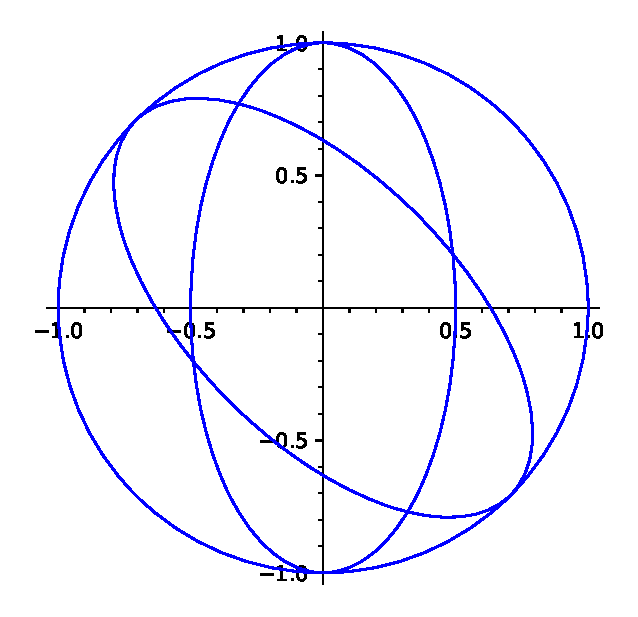
\includegraphics[scale = 0.5]{protbar.eps}
	\end{center}
	\end{figure}
	Abbiamo quindi che per $\mathcal R = \{R_{0}, R_{1}\}$ la norma euclidea standard è estrema, ma non è di Protasov perché ovviamente l'inviluppo convesso delle due ellissi non dà tutto il cerchio e non è nemmeno di Barabanov (si consideri ad esempio il punto $(1,0)$).
	
	Il punto $(3)$ segue dal formalismo della dualità, così come la prima equivalenza del punto $(4)$. Dimostriamo l'ultima equivalenza. $(\Rightarrow)$ che la norma sia estrema segue dal punto $(1)$. Sia ora $v\in\partial C$. Allora $\|v\| = 1$ e per definizione di norma di Barabanov esiste $R\in\mathcal R$ con $\tilde\rho^{-1}\|Rv\| = 1$, ma questo vuol dire che $\tilde\rho^{-1}Rv\in\partial C$. 
	$(\Leftarrow)$ Sia ora $v$ qualsiasi. Senza perdita di generalità, a meno di normalizzarlo possiamo supporre che valga $\|v\| = 1$. Vogliamo quindi dimostrare che $1 = \bigvee_{R\in\mathcal R}\tilde\rho^{-1}\|Rv\|$. Usando l'estremalità della norma abbiamo che
	$$\forall R\in\mathcal R,\; \tilde\rho^{-1}\|Rv\|\leq\tilde\rho^{-1}\|R\|\underbrace{\|v\|}_{=1} \leq \tilde\rho^{-1}\tilde\rho = 1.$$
	Per la disuguaglianza opposta, basta osservare che per la $R$ data dalla condizione si ha $\tilde\rho^{-1}\|Rv\| = 1$, quindi il sup deve essere almeno tale valore.
\end{proof}

\begin{osservazione}
	Nel punto $(4)$ non si chiede che $R$ sia invertibile. In effetti quanto detto funziona con le seminorme, ossia quelle per cui $\|v\|=0$ non implica $v = 0$. L'unica differenza è che in luogo dei CCB assorbenti si usano dei chiusi centrati assorbenti. Ad esempio si può considerare come ``corpo'' la striscia infinita $\R\times[-1,1]$. Esso induce la seminorma $\|(x,y)\| = |y|$. A questo punto considerando come $R = \begin{pmatrix}0 & 0 \\ 0 & 1\end{pmatrix}$ e come $C$ la palla unitaria standard (di $\R$, lungo l'asse $y$!), $R^{-1}C$ è proprio la striscia considerata. 
\end{osservazione}


Diamo ora un corollario ad un teorema della sezione precedente.
\begin{corollario}
	Sia $\mathcal R$ irriducibile. Allora esiste una norma di Protasov per $\mathcal R$.
\end{corollario}
\begin{proof}
	A meno di dividere per $\tilde\rho$ possiamo supporre senza perdita di generalità che $\tilde\rho = 1$. 
	Sia $E$ l'autoinsieme dato dal teorema, vediamo che $C = \conv(E)$ è di Protasov. Ovviamente è compatto, convesso e simmetrico. Inoltre, poiché lo span lineare di $E$ è tutto $\R^{n}$, $C$ è pure assorbente, quindi definisce una norma tramite il funzionale di Minkowski. 
	Bisogna verificare che è di Protasov, ossia che $C = \conv(\mathcal R(C))$. Si ha che 
	\begin{align*}
		\conv\left(\bigcup_{R\in\mathcal R}R[C]\right) &= 
		\conv\left(\bigcup_{R\in\mathcal R}R[\conv E]\right) = 
		\conv\left(\bigcup_{R\in\mathcal R}\conv(RE)\right) \overset{*}{=} \\ &= 
		\conv\left(\bigcup_{R\in\mathcal R}RE\right) = 
		\conv(\mathcal R[E]) = 
		\conv(E) = C.
	\end{align*}
	In $*$ basta osservare che un convesso contiene l'unione $A_{1}\cup\dots\cup A_{t}$ se e solo se contiene $\conv A_{1}\cup\dots\cup\conv A_{t}$, e nel passaggio seguente si usa il fatto che $E$ sia un autoinsieme.
\end{proof}

Analizziamo ora cosa succede considerando lo spazio duale $(\R^{n})^{*}$ identificato con $\R^{n}$ tramite $x\mapsto\langle x, -\rangle$ (attenzione: la $x$ di partenza è il funzionale, quella di arrivo il vettore che lo rappresenta). Un elemento del duale è un funzionale lineare $x:(\R^{n}, \|\cdot\|)\to(\R, |\cdot|)$, per cui la sua norma operatoriale, fissato un CCB $C$, è data da 
$$\|x\|^{*} = \max_{v\neq0}\frac{|\langle x, v\rangle|}{\|v\|} = \max_{\|v\|\leq1}|\langle x, v\rangle| = \max\langle x, C\rangle$$
dove nell'ultima espressione possiamo togliere il valore assoluto in quanto $C$ è simmetrico. 
Ha quindi senso definire il duale di un CCB come 
$$C^{*} = \{x: \|x\|^{*} = 1\} = \{x:\langle x, C\rangle \overset{(=)}{\leq} 1\}.$$
Vediamo ora che questa è una ``vera'' dualità.

\begin{proposizione}
	$C^{**} = C$.
\end{proposizione}
\begin{proof}
	Scriviamo per bene cos'è il biduale di un corpo convesso: 
	$$C^{**} = \{v: \langle C^{*}, v\rangle \leq 1\} = \{v:\forall x\in C^{*},\;\langle x,v\rangle\leq1\} = \{v:\forall x(\langle x,C\rangle\leq1\implies\langle x,v\rangle\leq1)\}.$$
	A questo punto $(\supseteq)$ è ovvio perché se $v\in C$ l'implicazione tra parentesi è automaticamente vera, per cui vediamo $(\subseteq)$. Ci occorre innanzitutto fare l'osservazione chiave che ogni CCB in $\R^{n}$ è l'intersezione di tutti i semispazi chiusi che lo contengono. Questo segue dal teorema di Hahn-Banach, che afferma che se $g:\R^{n}\to\R\geq0$ è subadditiva e $W$ è un sottospazio e $f:W\to\R$ è lineare con $|f|\leq g$, allora esiste $\tilde f$ che estende $f$ a tutto $\R^{n}$ ed è ancora dominata da $g$. 
	
	Nel nostro caso andiamo a dimostrare che $v\not\in C\implies v\not\in C^{**}$.
	Preso $v$, consideriamo il sottospazio $W:=\langle v\rangle$ e su di esso definiamo 
	$$f(sv) := s\|v\|,\quad s\in\R$$
	che è lineare, subadditiva e dominata: $|f(sv)|\leq\|sv\|$.
	Abbiamo allora che per H-B esiste $\tilde f$ che estende $f$, e che possiamo pensare come $\tilde f = \langle x, -\rangle$ per un qualche $x$, ancora dominata: $|\langle x, -\rangle|\leq \|-\|$.
	Tale $x$ testimonia che $v\not\in C^{**}$, infatti se $c\in C$ allora $|\langle x, c\rangle|\leq\| c\|\leq 1$ ma $|\langle x, v\rangle| = |f(v)| = \|v\|>1$ in quanto $v\not\in C$.
\end{proof}

Dato un IFS $\mathcal R$, ad esso si associa $\mathcal R^{T} = \{R^{T}:R\in\mathcal R\}$. Valgono allora alcune considerazioni riassunte nel seguente enunciato.
\begin{lemma}
	\begin{enumerate}
		\item $\mathcal R$ è irriducibile se e solo se $\mathcal R^{T}$ è irriducibile;
		\item $R[C]\subseteq C\iff R^{T}[C^{*}]\subseteq C^{*}$;
		\item $(R[C])^{*} = (R^{T})^{-1}[C^{*}]$ (anche se $R$ non è invertibile);
		\item $(\bigvee_{i} C_{i})^{*} = \bigcap_{i} C_{i}^{*}$.
	\end{enumerate}
\end{lemma}
\begin{proof}
	$(1)$ Sia $0<W<\R^{n}$ un sottospazio $\mathcal R$-invariante. Allora $W^{\perp}$ è proprio (ovvio per dimensionalità) e $\mathcal R^{T}$-invariante. Infatti presi $R\in\mathcal R$ e $v\in W^{\perp}$, si ha che 
	$$\forall w\in W,\; \langle R^{T}v, w\rangle = \langle v, Rw\rangle = 0$$
	in quanto $Rw\in W$ per ipotesi. L'altra implicazione si fa scambiando il ruolo di $\mathcal R$ e $\mathcal R^{T}$.
	$(2)$ è ovvio. 
	$(3)$ segue dalla seguente catena di equivalenze: 
	$$x\in(R[C])^{*} \iff \forall c\in C,\,\langle x, Rc\rangle\leq1\iff\forall c\in C,\,\langle R^{T}x, c\rangle\leq1\iff R^{T}x\in C^{*}.$$
	$(4)$ segue da 
	$$x\in\left(\bigvee_{i}C_{i}\right)^{*}\iff \forall v\in\conv\left(\bigcup_{i}C_{i}\right),\,\langle x,v\rangle\leq1\iff\forall v\in\bigcup_{i}C_{i},\,\langle x,v\rangle\leq 1.$$
\end{proof}

La dualità raggiunge il suo culmine nel seguente
\begin{lemma}[di Wirth]
	Sia $\mathcal R$ irriducibile. Allora $C$ è di Protasov [Barabanov] per $\mathcal R$ se e solo se $C^{*}$ è di Barabanov [Protasov] per $\mathcal R^{T}$.
\end{lemma}
\begin{proof}
	Il caso tra parentesi segue dall'altro gratis poiché $C^{**} = C$ e $\mathcal (R^{T})^{T} = \mathcal R$.
	
	Osserviamo che $\tilde\rho(\mathcal R) = \tilde\rho(\mathcal R^{T})$ e dunque senza perdita di generalità a meno di dividere possiamo supporre $\tilde\rho = 1$. Allora $C$ è di Protasov per $\mathcal R$ se e solo se (lemma) $C = \bigvee_{R\in\mathcal R}R[C]$ se e solo se (dualità)
	\begin{align*}
		C^{*} &= 
		\left(\bigvee_{R\in\mathcal R}R[C]\right)^{*} = 
		\bigcap_{R\in\mathcal R}(R[C])^{*} = 
		\bigcap_{R\in\mathcal R}(R^{T})^{-1}(C^{*}) = 
		\bigcap_{R\in\mathcal R^{T}}R^{-1}(C^{*})
	\end{align*}
	se e solo se (lemma) $C^{*}$ è di Barabanov per $\mathcal R^{T}$.
\end{proof}


\section{Trasformazioni frattali}

Siano dati $\mathcal R = \{R_{0},\dots,R_{N-1}\}$ e $\mathcal S = \{S_{0},\dots,S_{N-1}\}$ non necessariamente strettamente contrattivi, però tali per cui il teorema fondamentale degli IFS sia valido (il punto fondamentale è che $\forall\mathbf a\in\Omega$, $\bigcap_{n\geq0}K_{\mathbf a\upharpoonright n} = \{x\}$).

Consideriamo il seguente diagramma:
$$
\begin{tikzcd}
                                   & \Omega \arrow[ldd, "\pi_\mathcal R", two heads] \arrow[rdd, "\pi_\mathcal S", two heads] &              \\
                                   &                                                                    &              \\
K_\mathcal R \arrow[rr, "\varphi"] &                                                                    & K_\mathcal S
\end{tikzcd}
$$
Le due proiezioni sono suriettive per il teorema fondamentale (vale anche se l'IFS non è contrattivo, a patto di avere l'ipotesi fatta sopra). Vogliamo investigare le proprietà di $\varphi$. L'assunzione cruciale è che le fibre di $\pi_{\mathcal R}$ siano più fini di quelle di $\pi_{\mathcal S}$, ossia che 
$$\forall\mathbf a,\mathbf a'\in\Omega,\;\pi_{\mathcal R}(\mathbf a)= \pi_{\mathcal R}(\mathbf a')\implies \pi_{\mathcal S}(\mathbf a)= \pi_{\mathcal S}(\mathbf a').\quad (*)$$

\begin{lemma}
	Se vale $(*)$, allora $\varphi$ è ben definita e continua. Se inoltre $\pi_{\mathcal R}$ e $\pi_{\mathcal S}$ hanno le stesse fibre, allora $\varphi$ è un omeomorfismo.
\end{lemma}
\begin{proof}
	Consideriamo il seguente diagramma: 
	$$
	\begin{tikzcd}
                                              & \Omega \arrow[ldd, "\pi_\mathcal R", two heads] \arrow[rdd, "\pi_\mathcal S", two heads] \arrow[d, "\alpha", two heads] &              \\
                                              & \Omega/\equiv \arrow[ld, "\beta", two heads, tail] \arrow[rd, "\gamma", two heads]                &              \\
K_\mathcal R \arrow[rr, "\varphi", two heads] &                                                                                                   & K_\mathcal S
\end{tikzcd}
	$$
	Abbiamo posto $\equiv$ la relazione di equivalenza indotta dalle fibre di $\pi_{\mathcal R}$: 
	$$\mathbf a\equiv\mathbf a'\iff \pi_{\mathcal R}(\mathbf a) = \pi_{\mathcal R}(\mathbf a').$$
	Allora è evidente che da $(*)$ segue che $\gamma$ è suriettiva. 
	
	Poniamo ora su $\Omega/\equiv$ la topologia finale. (Ricordiamo cos'è: data $(X,\tau)\xrightarrow[]{F} Y$ con $F$ suriettiva, $A\subseteq Y$ è aperto nella topologia finale se e solo se $F^{-1}[A]$ è aperto in $(X,\tau)$.)
	Abbiamo che $\Omega/\equiv$ è compatto in quanto immagine suriettiva di un compatto, e inoltre che $\beta$ è continua.
	Infatti, dato $B\subseteq K_{\mathcal R}$ aperto, abbiamo che vale $\pi_{\mathcal R}^{-1}B = \alpha^{-1}(\beta^{-1}B)$ e $\beta^{-1}B$ è un aperto in $\Omega/\equiv$ per definizione di topologia finale perché $\pi_{\mathcal R}^{-1}B$ lo è in $\Omega$ per continuità di $\pi_{\mathcal R}$.
	Dunque $\beta$ è un omeomorfismo (per un teorema visto quando abbiamo parlato di funzioni proprie) e dire che $\varphi$ è continua equivale a dire che lo è $\gamma$. Questo fatto si dimostra come appena visto per $\beta$, per cui abbiamo finito.
	
	La seconda parte del teorema è ovvia.
\end{proof}

\begin{esempio}[scala del diavolo]
\end{esempio}


\subsection{Frazioni continue e mappa di Farey}

Consideriamo come al solito $\mathcal R = \{R_{0}, \dots, R_{N-1}\}$ per cui valga il teorema fondamentale degli IFS, e supponiamo di avere la seguente situazione.
$$\begin{tikzcd}
\Omega \arrow[r, "s", two heads] \arrow[d, "\pi", two heads] & \Omega \arrow[d, "\pi", two heads] \\
K \arrow[r, "F", dashed]                                     & K                                 
\end{tikzcd}$$
dove $s$ è l'operatore di shift (ossia tronca il primo simbolo della parola infinita).
Allora spesso si può definire $F$ (almeno su qualche sottoinsieme di $K$) in modo che il diagramma commuti. 
Se ciò è possibile, allora l'unico modo è quello tale che 
$$F\upharpoonright K_{a} = R_{a}^{-1}.$$
Infatti, se consideriamo $x = \pi(a\mathbf b) \overset{TF}{=} R_{a}(\pi(\mathbf b))$, abbiamo che 
$$F(x) = F(\pi(a\mathbf b)) = \pi(s(a\mathbf b)) = \pi(\mathbf b) = R_{a}^{-1}(x).$$
I problemi sorgono quando questa $F$ non è ben definita perché per due immagini vale ad esempio $K_{0}\cap K_{1}\neq\emptyset$, come capita con l'IFS dovuto a Farey,\dots.


\section{Gruppo di Möbius e geometria inversiva}

Sia $n\geq1$, definiamo 
$$\Pi^{n}:=\R^{n}\cup\{\infty\} \simeq S^{n}$$
dove l'isomorfismo è naturalmente dato dalla proiezione stereografica. 

Diamo alcune definizioni per $n=2$, ma si possono facilmente estendere a dimensioni arbitrarie. 
L'\emph{inversione di Möbius} rispetto alla retta $\langle y,w\rangle + \text{cost.} =0$ è data da 
$$x\mapsto x' = x - 2\frac{\langle x, w\rangle}{\langle w, w\rangle}w;$$
rispetto al cerchio di centro $w$ e raggio $r$ è definita implicitamente da 
$$\|x'-w\|\|x-w\| = r^{2},$$
ed esplicitamente da 
$$x\mapsto x' = w + \frac{r^{2}}{\|x-w\|^{2}}(x-w);$$
più in generale, per l'inversione rispetto a $S^{n-1}$ in $S^{n}$ si prende il cono tangente a $S^{n}$ in $S^{n-1}$ di vertice $w$ e, preso $x$, si traccia la retta per $x$ e $w$. L'immagine è l'altro punto di intersezione $x'$ di tale retta con $S^{n}$.

\begin{teorema}
	Sia $\Gamma$ la 2-sfera definita da $\|x-v\| = r$ in $\Pi^{3}$. Allora l'inversione $M$ rispetto a $\Gamma$:
	\begin{enumerate}
		\item fissa globalmente i 2-piani per $v$ ed agisce su di essi tramite l'inversione (nel piano) nella 1-sfera di centro $v$ e raggio $r$;
		\item scambia le 2-sfere per $v$ con i 2-piani non per $v$, e ciò avviene tramite proiezione stereografica rispetto a $v$;
		\item scambia le 2-sfere non per $v$ con altre 2-sfere non per $v$;
		\item per $0\leq m\leq 2$, conserva la classe di $m$-sfere e $m$-piani;
		\item è olomorfa (ossia conserva tutti gli angoli non orientati);
		\item distorce le distanze euclidee, ma conserva i birapporti;
		\item[1'.] fissa globalmente le 2-sfere perpendicolari a $\Gamma$ e agisce su di esse tramite inversione nella 1-sfera di intersezione con $\Gamma$.
	\end{enumerate}
\end{teorema}
\begin{proof}
	Il punto $(1)$ è ovvio. 
	D'ora in poi senza perdita di generalità possiamo supporre che $v = 0$, ossia che $\Gamma = \{y:\|y\| = r\}$. L'espressione esplicita dell'inversione diventa quindi $M(x) = \frac{r^{2}}{\|x\|^{2}}x$.
	Ora, l'equazione $$c\|x\|^{2} + \langle x,w\rangle + d = 0$$ descrive sia i 2-piani che le 2-sfere. Più precisamente si tratta di un 2-piano se e solo se $c = 0$; inoltre passa per $v = 0$ se e solo se $d = 0$. 
	Ora, se l'insieme $S$ è definito da tale equazione, vale 
	\begin{align*}
		M[S] &= 
		\{c\|M^{-1}x\|^{2} + \langle M^{-1}x, w\rangle + d = 0\} \\ &= 
		\{c\|Mx\|^{2} + \langle Mx, w\rangle + d = 0\}\\ &=
		\left\{c\left\|\frac{r^{2}x}{\|x\|^{2}}\right\|^{2} + \langle \frac{r^{2}x}{\|x\|^{2}}, w\rangle + d = 0\right\} \\&= 
		\left\{c\frac{r^{4}}{\|x\|^{2}} + \frac{r^{2}}{\|x\|^{2}}\langle x, w\rangle + d= 0\right\}\\ &= 
		\left\{\frac{d}{r^{2}}\|x\|^{2} + \langle x, w\rangle + cr^{2} = 0\right\}
	\end{align*}
	per cui la prima parte di $(2)$ segue da questa espressione. Per quanto riguarda l'azione come proiezione stereografica, bisogna osservare che qualunque retta per $v$ che taglia la sfera taglia anche il piano non per $v$ in un unico punto.
	
	Il punto $(3)$ segue dall'espressione per $M[S]$.
	
	Per quanto riguarda $(1')$, consideriamo una 2-sfera $\Sigma$ perpendicolare a $\Gamma$. Se dimostriamo che $\Sigma$ è fissata globalmente da $M$, l'affermazione segue; infatti la seconda parte è ovvia per definizione di inversione di una 2-sfera rispetto a un cerchio. 
	Supponiamo quindi che $\Sigma$ abbia centro $w$ e raggio $m$. La perpendicolarità $\Sigma\perp\Gamma$ impone, per Pitagora, che $$\|w\|^{2} = r^{2} + m^{2}.$$
	Dunque $\Sigma$ ha equazione $\|x-w\|^{2} = \|w\|^{2}-r^{2}$, che si traduce in 
	$$-\frac{1}{2}\|x\|^{2} + \langle x, w\rangle - \frac{r^{2}}{2} = 0.$$
	Quindi dall'espressione trovata prima segue che 
	\begin{align*}
		M[\Sigma] &= 
		\left\{\frac{-r^{2}/2}{2}\|x\|^{2} + \langle x, w\rangle + \left(-\frac{r^{2}}{2}\right) =0\right\} \\ &=
		\left\{-\frac{1}{2}\|x\|^{2} + \langle x,w\rangle - \frac{r^{2}}{2} = 0\right\} = \Sigma
	\end{align*}
	Il punto $(4)$ è ovvio. Per dimostrare $(5)$ consideriamo $u\neq 0, \infty$ e due vettori nello spazio tangente $v,w\in T_{u}\R^{3}$. Allora $M$ si fattorizza come 
	$$x\xrightarrow[]{Q} \|u\|^{2}\frac{x}{\|x\|^{2}}\xrightarrow[]{D_{\frac{r^{2}}{\|u\|^{2}}}} M(x),$$
	quindi basta verificare che $Q$ conservi gli angoli dato che ovviamente questo vale per la dilatazione. 
	Si può facilmente calcolare la jacobiana di $Q$, che in ogni punto è simmetrica. Inoltre valgono $Q(u) = u$ e $Q^{2} = \text{Id}$, per cui a livello di jacobiane vale 
	$$\text{Id} = J_{Q^{2}, u} = J_{Q, Q(u)}\cdot J_{Q, u} = J_{Q,u}^{2},$$
	quindi usando la simmetria della jacobiana 
	$$\langle J_{Q,u}v, J_{Q,u}w\rangle = \langle J_{Q,u}^{2}v, w\rangle = \langle \text{Id}v, w\rangle = \langle v,w\rangle$$
	cioè $Q$ conserva gli angoli come volevamo.
	
	Infine vediamo $(6)$ considerando la costruzione in figura. 
	\begin{figure}[htbp]
	\begin{center}
	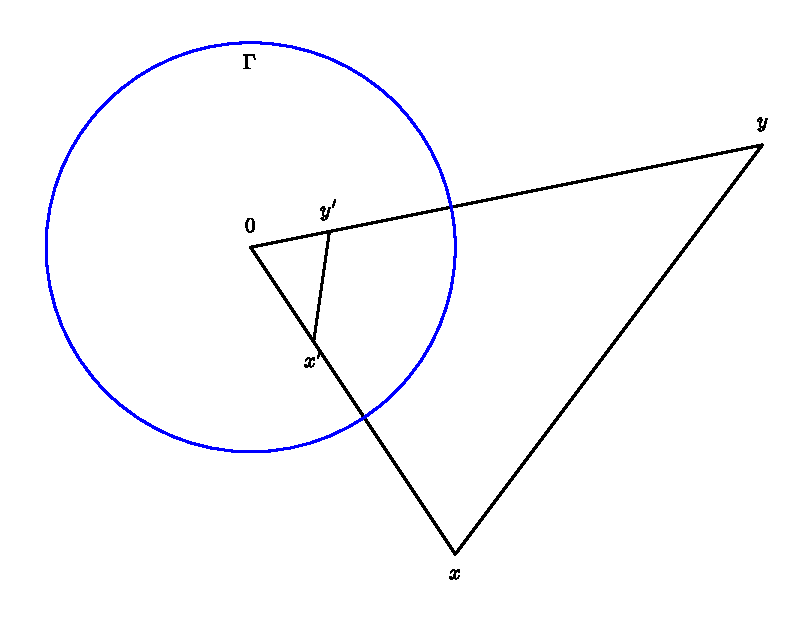
\includegraphics[scale = 0.6]{simili.eps}
	\end{center}
	\end{figure}
	I due triangoli sono simili, avendo un angolo in comune e valendo 
	$$\frac{\|x\|}{\|y'\|} = \frac{\|x\|}{r^{2}/\|y\|} = \frac{\|y\|}{r^{2}/\|x\|} = \frac{\|y\|}{\|x'\|}.$$
	Dunque 
	$$\|x'-y'\| = \|x-y\| \frac{\|y'\|}{\|x\|} = \frac{r^{2}}{\|x\|\|y\|}\|x-y\|,$$
	per cui \emph{in generale} la distanza euclidea non si conserva.
	A questo punto, scegliendo un birapporto (vale per tutti) si trova che
	$$\frac{\|z'-y'\|\|x'-w'\|}{\|z'-x'\|\|y'-w'\|} = \frac{\|z-y\|\frac{r^{2}}{\|z\|\|y\|}\|x-w\|\frac{r^{2}}{\|x\|\|w\|}}{\|z-x\|\frac{r^{2}}{\|z\|\|x\|}\|y-w\|\frac{r^{2}}{\|y\|\|w\|}} = \frac{\|z-y\|\|x-w\|}{\|z-x\|\|y-w\|}.$$
\end{proof}

Ci sono due conseguenze del risultato appena ottenuto. La prima è che dato un \emph{cerchio esteso} (ossia un vero cerchio o una retta) $C$ e un punto $x\not\in C$, l'immagine dell'inversione rispetto a tale cerchio può essere calcolata come l'intersezione della retta che congiunge $x$ con il centro di $C$ con l'unico cerchio (esteso) passante per $x$ e ortogonale a $C$. 
Infatti entrambi i cerchi estesi per $x$ sono fissati globalmente e si intersecano solo in $x$ e $x'$. 

La seconda conseguenza è che la proiezione stereografica coniuga le due definizioni di inversione, quella su $\Sigma^{n}$ e quella su $\Pi^{n}$.

(Fare disegni).

\begin{definizione}
	Dato $n\geq1$ e fissato di conseguenza $S^{n}$ (o equivalentemente $\Pi^{n}$), il \emph{gruppo di Möbius} $\Mob_{n}$ è il gruppo di biezioni di $S^{n}$ generato dalle inversioni nelle $n$-sfere perpendicolari al bordo di $S^{n}$ (o nel caso di $\Pi^{n}$, nelle $(n-1)$-sfere in cui queste intersecano $S^{n}$).
\end{definizione}

\begin{osservazione}
	Il gruppo di Möbius comprende traslazioni, rotazioni, simmetrie assiali e dilatazioni. Pensando in $\Pi^{n}$ è facile capirlo dato che l'inversione rispetto a rette non è altro che la simmetria assiale e con questa si generano rotazioni e traslazioni; le dilatazioni si ottengono invertendo rispetto a due cerchi concentrici.
	Ha un sottogruppo di indice 2, $\Mob_{n}^{+}$, che contiene gli elementi che preservano l'orientazione e si ottiene in modo ovvio moltiplicando un numero pari di elementi di $\Mob_{n}$.
\end{osservazione}

Concentriamoci ora sul caso di $n=2$. 
Dati $z\in\mathbb C\cup\{\infty\}$ e 
$$A=\begin{pmatrix}\alpha & \beta\\\gamma & \delta\end{pmatrix} \in PSL_{2}\mathbb C,$$
l'\emph{omografia indotta da $A$} è la mappa 
$$(A,0)(z) = \frac{\alpha z + \beta}{\gamma z + \delta}$$
mentre l'\emph{antiomografia indotta da $A$} è 
$$(A,1)(z) = \frac{\alpha \bar z + \beta}{\gamma \bar z + \delta}.$$
Risulta evidente che valga il seguente schema per le composizioni di due [anti]omografie:
\begin{align*}
	(A,0)\circ(B,0) &= (AB,0)\\
	(A,0)\circ(B,1) &= (AB,1)\\
	(A,1)\circ(B,0) &= (A\bar B,1)\\
	(A,1)\circ(B,1) &= (A\bar B,0)
\end{align*}
per cui il gruppo di omografie e antiomografie è $PSL_{2}\mathbb C\rtimes \mathbb Z_{2}$.

\begin{osservazione}
	Fissato un cap $\mathcal H^{n}$ di $S^{n}$, sia $\stab(\mathcal H^{n},\Mob_{n})$ il suo stabilizzatore in $\Mob_{n}$. Una volta dimostrato che tale stabilizzatore è generato dalle inversioni rispetto a cerchi perpendicolari al bordo di $\mathcal H^{n}$, dato che queste generano $\Mob_{n-1}$ risulterà $\stab(\mathcal H^{n}, \Mob_{n})\simeq\Mob_{n-1}$.
\end{osservazione}

\begin{lemma}[decomposizione di Iwasawa]
	Ogni $M\in SL_{2}\mathbb C$ è scrivibile in modo unico come $M = KAN$ dove $K \in \mathcal K = SU_{2}\mathbb C$, $A \in \mathcal U = \{\begin{pmatrix}a & 0\\ 0 & a^{-1}\end{pmatrix},\,a>0\}$ e $N\in\mathcal N = \{\begin{pmatrix}1 & \beta\\ 0 & 1\end{pmatrix},\,\beta\in\mathbb C\}$.
\end{lemma}
\begin{proof}
	Consideriamo l'immagine della base canonica tramite $M$, 
	$$(e_{1}, e_{2})M = (m_{1}, m_{2})$$
	e fissato $u_{1} = m_{1}$ imponiamo l'ortogonalità con $u_{2} = m_{2}-\alpha m_{1}$, ossia $\langle m_{1}, m_{2}-\alpha m_{1}\rangle = 0$, che determina $\alpha = \langle m_{1}, m_{2}\rangle /\langle m_{1}, m_{1}\rangle$. Abbiamo quindi la seguente relazione
	$$(u_{1}, u_{2}) = (m_{1},m_{2}) \underbrace{\begin{pmatrix}1 & -\alpha\\ 0 & 1\end{pmatrix}}_{=:N^{-1}}.$$
	La nuova base è ortogonale, quindi poiché 
	$$(e_{1}, e_{2}) MN^{-1} = (u_{1},u_{2})$$
	la matrice $MN^{-1}$ è ortogonale (non per forza hermitiana!). Di conseguenza esiste $a>0$ tale che 
	$$(MN^{-1})^{*}(MN^{-1}) = \begin{pmatrix}a^{2} & 0\\ 0 & a^{-2}\end{pmatrix} =: A^{2}$$
	per cui 
	$$(MN^{-1}A^{-1})^{*}(MN^{-1}A^{-1}) = I_{2}$$
	e quindi $MN^{-1}A^{-1} =: K\in\mathcal K$, e abbiamo dimostrato l'esistenza.
	
	Per quanto riguarda l'unicità della decomposizione, supponiamo che $K_{1}A_{1}N_{1} = K_{2}A_{2}N_{2}$. 
	Allora 
	$$N_{1}^{*}A_{1}^{*}\underbrace{K_{1}^{*}K_{1}}_{=I_{2}}A_{1}N_{1} = N_{2}^{*}A_{2}^{*}\underbrace{K_{2}^{*}K_{2}}_{=I_{2}}A_{2}N_{2}$$
	per cui dal fatto che le $A_{i}$ sono diagonali a elementi reali si ha $A_{i}^{*} = A_{i}$, quindi 
	$$N_{1}^{*}A_{1}^{2}N_{1} = N_{2}^{*}A_{2}^{2}N_{2}.$$
	A questo punto moltiplichiamo a sinistra per $(N_{2}^{*})^{-1}$ e a destra per $N_{1}^{-1}$, ottenendo
	$$(N_{2}^{*})^{-1} N_{1}^{*} A_{1}^{2} = A_{2}^{2} N_{2}N_{1}^{-1}$$
	e qui il termine a sinistra è triangolare inferiore, quello a destra triangolare superiore. Di conseguenza entrambi devono in realtà essere diagonali, da cui seguono $N_{1} = N_{2}$ e $A_{1} = A_{2}$. 
\end{proof}

\begin{teorema}
	Vale $\Mob_{2} = PSL_{2}\mathbb C\rtimes\mathbb Z_{2}$, e di conseguenza $\Mob_{2}^{+} = PSL_{2}\mathbb C$.
\end{teorema}
\begin{proof}
	$(\subseteq)$ L'inversione rispetto alla circonferenza unitaria centrata nell'origine è data da 
	$$z\mapsto \frac{1}{\bar z} = \left(\begin{pmatrix}0 & i\\ i & 0\end{pmatrix}, 1\right)$$
	per cui è un'antiomografia. 
	La dilatazione di un generico fattore $r>0$ è data da 
	$$\left(\begin{pmatrix}r^{1/2} & 0\\ 0 & r^{-1/2}\end{pmatrix}, 0\right),$$
	la traslazione di $\alpha\in\mathbb C$ da 
	$$\left(\begin{pmatrix}1 & \alpha\\ 0 & 1\end{pmatrix}, 0\right)$$
	e quindi per le inversioni rispetto a cerchi va tutto bene. 
	Per quanto riguarda le inversioni rispetto a rette, sono tutte coniugate (a meno di rototraslazione) a quella rispetto all'asse reale, e questa è indotta da 
	$$\left(\begin{pmatrix}1 & 0\\ 0 & 1\end{pmatrix}, 1\right).$$
	
	$(\supseteq)$ Si utilizza la decomposizione di Iwasawa per elementi di $SL_{2}\mathbb C$, per cui preso un generico $M\in SL_{2}\mathbb C$ abbiamo $M = KAN$. Abbiamo che $A,N\in \Mob_{2}$, per cui ci resta da determinarlo per $K\in SU_{2}\mathbb C$.
	Studiamo meglio la forma di $K = \begin{pmatrix}\alpha & \beta \\\gamma & \delta\end{pmatrix}$.
	Dato che sta in $SU_{2}\mathbb C$, deve valere $K^{-1} = K^{*}$ che si traduce in termini di elementi come $\delta = \bar\alpha$ e $\gamma = -\bar\beta$, per cui abbiamo che 
	$$\begin{pmatrix}\alpha & \beta \\ -\bar\beta & \bar\alpha\end{pmatrix},\quad \det K = |\alpha|^{2} + |\beta|^{2} = 1.$$
	Se $K\neq\pm \text{Id}$, ci sono due autovalori complessi coniugati di modulo 1 e due corrispondenti autovettori. 
	
	Osserviamo ora che $\forall p,q\in P^{1}\mathbb C$ esiste un elemento $B$ di $\Mob_{2}$ che manda $p\mapsto\infty$ e $q\mapsto1$. Infatti se $p=\infty$ basta applicare una traslazione, se $p\neq\infty$ si considera l'inversione rispetto alla circonferenza di centro $p$ e passante per $q$ e si ricade nel caso procedente.
	
	Possiamo quindi supporre senza perdita di generalità che gli autovettori di $K$ siano $1$ e $\infty$. L'equazione che testimonia questo fatto è 
	$$BKB^{-1}\begin{pmatrix}1 & 0\\ 0& 1\end{pmatrix} = \begin{pmatrix}\rho & 0\\ 0& \bar\rho\end{pmatrix}\begin{pmatrix}1 & 0\\ 0& 1\end{pmatrix} $$
	e osserviamo che la penultima matrice è una rotazione di angolo $2\text{arg}(\rho)$, che sta in $\Mob_{2}$. Quindi $K\in\Mob_{2}$.
\end{proof}

Lo spazio iperbolico $\mathcal H^{3}$ si può pensare in due modi: come l'interno di una sfera $S^{2}$ (che sarebbe un cap di $S^{3}$) oppure grazie alla proiezione stereografica come la parte ``sopra'' al piano $\mathbb C\cup\{\infty\}$. 
La distanza che si usa è quella iperbolica, definita inizialmente per il modello di Klein di $\mathcal H^{2}$ ma che va bene anche per gli altri casi, data da 
$$d_{B}(p_{1}, p_{2}) = \log\frac{\|p_{0} - p_{2}\|\|p_{1} - p_{3}\|}{\|p_{0} - p_{1}\|\|p_{2} - p_{3}\|}$$
dove $p_{0}$ e $p_{3}$ sono i punti che si ottengono facendo l'intersezione dell'unico $1$-cerchio per $p_{1}$ e $p_{2}$ perpendicolare a $\partial \mathcal H^{2}$ (o $\partial \mathcal H^{3}$) con tale bordo. 
Poiché le inversioni conservano il birapporto, gli elementi di $\Mob_{2}$ (o $\Mob_{3}$) sono isometrie per lo spazio iperbolico. Precisiamo questo fatto nel seguente teorema.

\begin{teorema}
	Ogni isometria di $\mathcal H^{3}$ è nel sottogruppo di $\Mob_{3}$ generato dalle inversioni nelle 2-sfere perpendicolari a $\partial\mathcal H^{3}$ (più in generale per il caso di $\mathcal H^{n}$ bastano $n+1$ inversioni). In particolare, tale sottogruppo è proprio $\stab (\mathcal H^{3}, \Mob_{3})$.
\end{teorema}
\begin{proof}[Schema di dimostrazione]
	Per omogeneità, un'isometria è determinata dalla sua azione su un qualsiasi simplesso dello spazio. 
	Preso dunque un tetraedro di vertici $p_{0}, p_{1}, p_{2}, p_{3}$ e un'isometria $\Phi$, diciamo che le immagini dei vertici del tetraedro siano $q_{0}, q_{1}, q_{2}, q_{3}$. 
	Si manda dunque $p_{0}\mapsto q_{0}$ con un'opportuna inversione (questo è facile!). 
	Dopodiché si prende un'inversione che manda $p_{1}\mapsto q_{1}$ ma la cui sfera contiene $q_{0}$, che quindi resta fissato, e così avanti. 
	Si riesce giusto in tempo perché c'è solo una sfera per tre punti e perpendicolare al bordo, ma è proprio quella che scambia tra loro i due possibili tetraedri costruiti sulle immagini dei primi tre punti.
\end{proof}

$$
\begin{tikzcd}[cramped, column sep = small]
                                             & \Mob_3 \arrow[d, no head]                                                                                                               &                                                                    \\
                                             & PSL_2\mathbb C\rtimes\mathbb Z_2 = \Mob_2 = \stab\mathcal H^3 = \text{Iso}^\pm\mathcal H^3 \arrow[ld, "2", no head] \arrow[rd, no head] &                                                                    \\
PSL_2\mathbb C = \Mob_2^+ \arrow[rd, "(**)", no head] &                                                                                                                                        & \Mob_1 = \stab\mathcal H^2 = PSL_2\mathbb R\rtimes\mathbb Z_{2} \arrow[ld, "(*)", no head] \\
                                             & \Mob_1^+ = PSL_2\mathbb R                                                                                                               &                                                                   
\end{tikzcd}
$$

\begin{osservazione}
	Consideriamo un generico $z\in\mathbb C$. Esso appartiene a $\mathcal H^{2}$ se e solo se 
	$$\begin{pmatrix}z \\ 1\end{pmatrix}^{*} \begin{pmatrix}0 & -i \\ i & 0\end{pmatrix} \begin{pmatrix}z \\ 1\end{pmatrix}<0.$$
	Infatti svolgendo i conti si ottiene che tale condizione equivale a 
	$$-i\bar z + iz = i(z-\bar z) = i2\Im z\cdot i = -2\Im z < 0.$$
	Ne segue che una generica matrice $A = \begin{pmatrix}\alpha & \beta \\ \gamma & \delta\end{pmatrix}\in PSL_{2}\mathbb C$ stabilizza globalmente il piano iperbolico $\mathcal H^{2}$ (considerato nel modello del semipiano) se e solo se lascia invariata tale forma, ossia 
	$$A^{*}\begin{pmatrix}0 & -i \\ i & 0\end{pmatrix}A = \begin{pmatrix}0 & -i \\ i & 0\end{pmatrix}.$$
	(In realtà questa relazione dovrebbe valere a meno di costante moltiplicativa perché quello che ci interessa è soltanto che il segno della forma resti invariato, ma la costante moltiplicativa si può sempre assorbire nella matrice di $PSL_{2}\mathbb C$).
	Svolgendo i calcoli si ottiene che ciò equivale a $\alpha, \beta,\gamma,\delta\in\R$, che dimostra $(**)$ nel reticolo qui sopra.
	
	Per tornare al piano di sopra dall'altro lato $(*)$, bisogna aggiungere l'inversione $z\mapsto -\bar z$, che è indotta da 
	$$\left(\begin{pmatrix}i & 0 \\ 0 & i^{-1}\end{pmatrix}, 1\right)$$
	ma anche da 
	$$\left(\begin{pmatrix}-1 & 0 \\ 0 & 1\end{pmatrix}, 1\right)$$
	che è una scelta più furba perché permette di non uscire dai reali.
\end{osservazione}

\subsection{Gruppi fuchsiani/kleiniani}

\begin{lemma}
	Sia $\mathcal G$ un gruppo che agisce in modo transitivo sullo spazio topologico di Hausdorff localmente compatto $X$. Le due condizioni seguenti sono equivalenti e definiscono un'\emph{azione propriamente discontinua}:
	\begin{enumerate}
		\item $\forall x\in X,\;\forall K\subseteq X$ compatto, $\#\{G\in\mathcal G:\,Gx\in K\}<\infty$;
		\item l'orbita di ogni $x\in X$ è discreta e ogni punto ha stabilizzatore finito. 
	\end{enumerate}
\end{lemma}
\begin{proof}
	$(1\implies 2)$ Che lo stabilizzatore sia finito si ottiene facilmente scegliendo $K = \{x\}$. 
	Ora, visto che l'azione è transitiva, basta dimostrare che $\forall x\in X,\,\exists O\ni x$ aperto con $O\cap \mathcal G*x = \{x\}$.
	Per la locale compattezza, questo $O$ si può scegliere in modo che la sua chiusura sia compatta. Per $(1)$ però questo implica che tale chiusura contenga un numero finito di punti dell'orbita. Quindi qui fissato un particolare punto dell'orbita, esso si può separare dagli altri grazie all'ipotesi che lo spazio sia di Hausdorff. 
	
	$(2\implies1)$ Dati $x$ e $K$, per ipotesi abbiamo che $\mathcal G*x$ è discreta. Poiché $K$ è compatto, l'intersezione $\mathcal G*x\cap K$ è finita. Infine la cardinalità dell'insieme delle mappe da $x$ a un certo $y$ è la stessa dello stabilizzatore di $y$, che per ipotesi è finito. Di conseguenza è finita anche la cardinalità dell'insieme delle mappe che mandano $x$ nei punti di $\mathcal G*x\cap K$, in quanto unione finita di insiemi finiti.
\end{proof}

\begin{osservazione}
	Se $\mathcal G$ è anche un gruppo topologico e l'azione è continua e propria (cioè i controinsiemi di compatti sono compatti, rispetto alla mappa $G\times X\to X$) e consideriamo un sottogruppo $\Gamma\leq\mathcal G$ discreto, allora l'azione di $\Gamma$ su $X$ è propriamente discontinua. 
\end{osservazione}
\begin{proof}
	Verifichiamo la condizione 1 del lemma, ossia che dati $x$ e $K$, l'insieme $\{G\in\Gamma:\, Gx\in K\}$ è finito. 
	Tale insieme si può riscrivere come 
	$$\Gamma\cap \{G\in\mathcal G:\, Gx\in K\} = \Gamma \cap \{(G,y)\in\mathcal G\times X:\,Gy\in K\}\cap \pi^{-1}\{x\}$$
	e siccome l'azione è propria, $\{(G,y):\,Gy\in K\}$ è compatto; inoltre $\pi^{-1}\{x\}$ è chiuso, per cui anche l'intersezione $\{(G,y):\,Gy\in K\}\cap \pi^{-1}\{x\}$ è compatta essendo un chiuso in un compatto. Infine, essendo $\Gamma$ discreto, ovviamente intersecandolo con un compatto si ottiene un insieme finito.
\end{proof}

\begin{definizione}
	Un sottogruppo $\Gamma$ di $\Mob_{n-1}$ che agisce in modo propriamente discontinuo su $\mathcal H^{n}$ si dice un \emph{gruppo fuchsiano esteso} se $n=2$ (ossia è un sottogruppo di $PSL_{2}\R\rtimes\mathbb Z_{2}$), un \emph{gruppo kleiniano esteso} se $n=3$ (sottogruppo di $PSL_{2}\mathbb C\rtimes\mathbb Z_{2}$). I loro sottogruppi che preservano l'orientazione si dicono \emph{gruppi fuchsiani} e \emph{kleiniani} rispettivamente. 
\end{definizione}

\begin{esempio}
	$PSL_{2}\mathbb Z$ e $PSL_{2}\mathbb Z\rtimes\mathbb Z_{2}$ sono fuchsiani; il gruppo modulare di Picard $PSL_{2}\mathbb Z[i]$ è kleiniano. Esempi più generali si hanno considerando i vari $PSL_{2}\mathbb O$, dove $\mathbb O$ è l'anello degli interi algebrici di una fissata estensione quadratica complessa di $\mathbb Q$, detti gruppi di Bianchi.
	Le estensioni quadratiche \emph{reali} non vanno bene, perché se ad esempio abbiamo $\mathbb Q(\lambda)$ di grado 2, vale 
	$$
	\begin{pmatrix}
	1 & \lambda^{-k}\\
	0 & 1
	\end{pmatrix}
	\xrightarrow[]{k\to\infty}
	\begin{pmatrix}
	1 & 0\\
	0 & 1
	\end{pmatrix}$$
	quindi l'identità $I_{2}$ è punto di accumulazione, per cui non si possono avere orbite discrete.
\end{esempio}

\subsection{Classificazione inversioni}

Abbiamo visto che i gruppi $\text{Mob}_1^+$ e $\text{Mob}_2^+$ sono isomorfi a $PSL_2\mathbb R$ e $PSL_2 \mathbb C$ rispettivamente. 
Vogliamo classificare le trasformazioni di tali gruppi, e lo facciamo per il più grande (la classificazione delle trasformazioni di $PSL_2\mathbb R$ sarà una conseguenza di questa).

Consideriamo quindi una generica matrice 
$$A = \begin{pmatrix}\alpha & \beta \\ \gamma & \delta\end{pmatrix}\in PSL_2\mathbb C.$$
Essa agisce in modo naturale su $P^1\mathbb C$ e per estensione anche su $\mathcal H^3$ pensato come lo spazio "sopra" a $P^1\mathbb C$.

\begin{osservazione}
In effetti possiamo pensare ad $\mathcal H^3$ come ad un sottoinsieme dei quaternioni $\mathbb H$, in particolare quello dei quaternioni della forma 
$$q = z + rj,\quad z\in\mathbb C,\, r>0.$$
A questo punto l'inversione rispetto ad una circonferenza di $P^1\mathbb C$ agisce su $\mathcal H^3$ come l'inversione rispetto alla (unica) sfera che ha tale circonferenza come equatore. 
Algebricamente, ricordando che i quaternioni non sono commutativi, l'azione della matrice $A$ definita sopra si esprime come 
$$A*q = (\alpha q + \beta)(\gamma q + \delta)^{-1}.$$
\end{osservazione}

Vediamo che la classificazione di tali trasformazioni dipende essenzialmente dalla traccia della matrice, $t := \alpha + \delta$.
Essendo il polinomio caratteristico dato da $x^2 - tx + 1$, gli autovalori di $A$ sono $\frac{t\pm\sqrt{t^2 - 4}}{2}$. Distinguiamo alcuni casi.
\begin{itemize}
    \item $t^2 = 4$, ovvero $t = \pm2$. Abbiamo allora un unico autovalore che vale $\pm1$ e $A$ risulta coniugata a 
    $$\begin{pmatrix}1 & 1\\0 & 1\end{pmatrix}$$
    che (sul piano) agisce come una traslazione euclidea. $A$ in questo caso si dice \emph{parabolica}.
    \item $t\in(-2, 2)\subset\mathbb R$. Allora gli autovalori sono $\rho$ e $\bar\rho$ e la matrice $A$ è coniugata a 
    $$\begin{pmatrix}\rho & 0\\0 & \bar\rho\end{pmatrix}$$
    che agisce sul piano come una rotazione $z\mapsto \rho^2 z$. 
    $A$ si dice \emph{ellittica}.
    \item $t\in\mathbb C\setminus [-2,2]$. Allora gli autovalori sono $\rho$ e $\rho^{-1}$ con $|\rho|>1$, $A$ è coniugata a 
    $$\begin{pmatrix}\rho & 0\\0 & \rho^{-1}\end{pmatrix}$$
    e agisce come una rotodilatazione $z\mapsto\rho^2 z$. $A$ si dice \emph{lossodromica}.
    Un sottocaso particolare di questo si ha quando $t\in\mathbb R\setminus [-2,2]$, nel qual caso $A$ si dice \emph{iperbolica} (e infatti per le matrici di $PSL_2\mathbb R$ di solito si parla solo di queste ultime).
\end{itemize}

\subsection{Insiemi limite}
\begin{definizione}
    Sia $\Gamma<PSL_2\mathbb C$ kleiniano. Il suo \emph{insieme limite} è 
    $$\Lambda = \Lambda(\Gamma) = \{p\in\partial\mathcal H^3:\; 
    \exists q\in\mathcal H^3 \text{ t.c. $p$ è di accumulazione per l'orbita $\Gamma*q$ di $q$}\}.$$
\end{definizione}

Importante: nella definizione appena data, l'accumulazione si intende rispetto alla norma euclidea. 

\begin{osservazione}
    Se $p$ è di accumulazione per $\Gamma*q$, allora lo è pure per $\Gamma*t$.
\end{osservazione}
\begin{proof}
    Se $p$ è di accumulazione per $\Gamma*q$, allora esiste una successione $G_0,G_1,\dots\in\Gamma$ tale che $G_n*q\to p$ in senso euclideo per $n\to\infty$.
    Consideriamo l'orbita $G_n*t$. Poiché le $G_n$ stanno in $PSL_2\mathbb C$, esse conservano la distanza iperbolica. Quindi se $d$ è la distanza iperbolica tra $q$ e $t$, è anche la distanza iperbolica tra $G_n q$ e $G_n t$ per ogni $n$. Però siccome il punto di accumulazione $p$ di $\Gamma*q$ sta sul bordo $\partial\mathcal H^3$, tali distanze in senso euclideo vanno a 0, per cui si può concludere per la disuguaglianza triangolare che $G_n * t\to p$.
\end{proof}

\begin{osservazione}
    Ovviamente $\Lambda$ è un chiuso perché il suo complementare $\Omega = \partial\mathcal H^3\setminus \Lambda$, detto anche \emph{insieme regolare} o \emph{dominio di discontinuità} di $\Gamma$ è aperto. 
    Altrettanto ovviamente $\Lambda$ è $\Gamma$-invariante, e gli elementi di $\Gamma$ agiscono su $\Lambda$ come omeomorfismi.
    Una proprietà meno ovvia è che se $\Lambda$ non ricade in alcuni casi speciali (vuoto, un punto, due punti, $\partial\mathcal H^{3}$) allora è un \emph{perfetto} (chiuso senza punti di accumulazione) ad interno vuoto.
\end{osservazione}
\begin{esempio}
	Le rotazioni non hanno punti di accumulazione sul bordo; le lossodromiche ne hanno due; il gruppo di inversioni generato da quelle in cerchi con diametri tutti lungo una circonferenza massima di $\partial \mathcal H^{3}$ ha come insieme limite la circonferenza massima stessa; il gruppo di Picard ha (probabilmente) $\Lambda = \partial \mathcal H^{3}$.
\end{esempio}


\subsection{Unificazione di cap e punti}

Consideriamo ora il gruppo (fuchsiano esteso) generato dalle inversioni rispetto a tre cerchi disgiunti in $P_1\mathbb C$ (o in alternativa in $S^{2}$).
Vogliamo studiare il suo comportamento utilizzando il chaos game. 
Siccome le trasformazioni che andiamo ad applicare sono involuzioni, è importante non applicare due volte consecutive la stessa. Questo obiettivo si può raggiungere facilmente se l'indice della "nuova" trasformazione da applicare si ottiene sommando 1 o 2 e poi facendo mod 3.

Se usassimo un gruppo fuchsiano tipo 
$$\Gamma = \langle A_0, \dots, A_{N-1}, A_0^{-1},\dots, A_{N-1}^{-1}\rangle$$
avremmo il problema simile di evitare di applicare una trasformazione e la sua inversa consecutivamente. 

Vediamo ora una interessante costruzione che permette di rendere tutto più semplice. 
Consideriamo la sfera $S^n$. Ad un suo cap $C$ si può associare il suo centro $c\in S^n$ e l'angolo di apertura $\theta\in(0,\pi)$.
Allora il cap si può caratterizzare come 
\begin{align*}
    C &= \{x\in S^n:\; \langle x, c\rangle \geq\cos\theta\} = 
    \{x\in S^n:\; \langle x, c\rangle -\cos\theta\geq 0\} \\&= 
    \{x\in S^n:\; \langle x, \frac{c}{\sin\theta}\rangle - \cot\theta\geq 0\}.
\end{align*}
A questo punto descriviamo sia i punti che i caps come dei vettori in $\mathbb R^{n+2}$ tramite le seguenti associazioni: 
\begin{itemize}
    \item $x\in S^n$ viene associato a $\mathbf{x} = (x_1,\dots,x_{n+1}, 1)^t$;
    \item $C\sim(c,\theta)$ viene associato a $\mathbf{w} = (c_1/\sin\theta,\dots,c_{n+1}/\sin\theta, \cot\theta)^t$.
\end{itemize}
D'ora in avanti useremo $\langle-,-\rangle$ anche per vettori in $\mathbb R^{n+2}$ indicando il prodotto scalare di Lorentz di segnatura $(n+1,1)$. Dal contesto (vettori in grassetto) sarà sempre chiaro quale stiamo usando. 

Con queste convenzioni, abbiamo le seguenti conseguenze: 
\begin{itemize}
    \item $x\in C$ se e solo se $\langle \mathbf{x}, \mathbf{w}\rangle \geq0$;
    \item $\mathbf x\in\mathbb R^{n+2}$ corrisponde ad un punto se e solo se $\mathbf x_{n+1} = 1$ e $\langle\mathbf{x}, \mathbf{x}\rangle = 0$;
    \item $\mathbf{w}\in\mathbb R^{n+2}$ corrisponde ad un cap se e solo se appartiene allo \emph{spazio di De Sitter} $S= \{\mathbf z\in\mathbb R^{n+2}:\;\langle\mathbf{z}, \mathbf{z}\rangle = 1\}$.
\end{itemize}
\begin{proof}
    Dimostriamo solo l'ultima equivalenza. $(\Rightarrow)$ è immediato: 
    $$\left(\frac{c_1}{\sin\theta}\right)^2+\dots + \left(\frac{c_{n+1}}{\sin\theta}\right)^2 - (\cot\theta)^2 = \frac{1-(\cos\theta)^2}{(\sin\theta)^2} = 1.$$
    Vediamo $(\Leftarrow)$. Sia $\mathbf y$ tale che $\langle\mathbf{y}, \mathbf{y}\rangle = 1$. Basta porre $\theta = \text{arccot} y_{n+2}$ e di conseguenza, dato che il centro del cap deve appartenere alla sfera, $c:=(y_1,\dots,y_{n+1})/(1 + y_{n+2}^2)^{1/2}$.
\end{proof}

La magia di tutta questa costruzione sta nel seguente risultato. 
\begin{teorema}
L'inversione rispetto a $C\sim \mathbf w$ è data da 
$$\mathbf x\mapsto\mathbf x - 2\langle\mathbf{w}, \mathbf{x}\rangle\cdot\mathbf w$$
\end{teorema}

Tale mappa se consideriamo come ambiente $S^2$ è un elemento di $GL_4\mathbb R$, più precisamente di $O_{3,1} \mathbb R$. La cosa importante è che possiamo scriverla in modo esplicito(!), infatti preso un punto $\mathbf x = (x_1,x_2, x_3, 1)^t$ la sua immagine è 
$$I\mathbf x - 2 \mathbf w\mathbf w^t\begin{pmatrix}1 & & & \\ & 1 & & \\ & & 1 & \\ & & & -1\end{pmatrix}\mathbf x = [I - 2 \mathbf w\mathbf w^t L]\mathbf x.$$

Esercizio in SageMath: consideriamo inizialmente i tre cap corrispondenti a $\mathbf w_0 = (0, 1, -1, 1)^t$, $\mathbf w_1 = (0, -1, -1, 1)^t$, $\mathbf w_0 = (0, -1, 1, 1)^t$ e usiamo il chaos game su questi. Infine aggiungiamo un cap parametrico $\mathbf w_4 = (1/\sin\theta, 0, 0, \cot\theta)$ e facciamo variare $\theta$ facendolo crescere fino a quando il cap corrispondente non è tangente agli altri tre.  


\begin{teorema}
	L'inversione nel cap $C\sim \mathbf w$ è data dalla mappa
	$$\mathbf x\mapsto\mathbf x - 2 \frac{\langle \mathbf w, \mathbf x\rangle}{\langle \mathbf w, \mathbf w\rangle}\mathbf w.$$
	Tale mappa è un elemento di $O_{3,1}\R$, e tale espressione funziona sia per i punti che per i cap.
\end{teorema}
\begin{proof}
	Dati $S^{3}$ e $\mathbf w$, osserviamo che $\langle \mathbf x,\mathbf w\rangle = 0$ individua il piano polare a $\mathbf w$ rispetto alla conica $S^{3}$. 
	Allora preso un generico $\mathbf x$, possiamo scriverlo in modo unico come $\mathbf x = \mathbf u + r\mathbf w$ con $\mathbf u$ in tale piano polare. La sua immagine tramite la mappa definita nell'enunciato è $\mathbf x' = \mathbf u-r\mathbf w$. 
	Osserviamo che $\mathbf x\mapsto\mathbf x'$ conserva la forma di Lorentz (esercizio), per cui se dimostriamo che i tre punti $x,x',w$ (corrispondenti nello spazio di partenza di $\mathbf x,\mathbf x'$, con l'ultimo che è il ``vertice'' del cap corrispondente a $\mathbf w$) sono allineati allora $x'$ è proprio l'immagine di $x$ tramite l'inversione nel cap $C_{\mathbf w}$, in quanto valgono $\langle \mathbf x',\mathbf x'\rangle = \langle \mathbf x,\mathbf x\rangle = 0$ e l'intersezione di una retta con $S^{2}$ ha due punti (ricordare la costruzione geometrica dell'inversione!). 
	Che siano allineati si ottiene considerando il fatto che $\mathbf x' = \mathbf x - 2 \frac{\langle \mathbf w, \mathbf x\rangle}{\langle \mathbf w, \mathbf w\rangle}\mathbf w$, per cui $\mathbf x',\mathbf x,\mathbf w$ stanno sullo stesso 2-piano e quindi $x,x',w$ sulla stessa retta proiettiva.
	
	La stessa formula funziona anche per i cap perché conserva la forma di Lorentz e quindi manda cap in cap. Inoltre, per lo stesso motivo, manda $\mathbf x\in C_{\mathbf w}$ in $\mathbf x'\in C_{\mathbf w'}$, dato che l'appartenenza ad un cap si esprime in termini di forma di Lorentz.
\end{proof}


\begin{lemma}
	Sia $A\in O_{3,1}\R$. Allora $a_{44}\neq0$ e $A$ fissa globalmente ognuna delle due componenti connesse $\pm\mathcal L$ di $\{\mathbf x:\langle \mathbf x,\mathbf x\rangle = -1\}$ oppure le scambia a seconda del segno di $a_{44}$.
	Di conseguenza l'omomorfismo 
	$$O_{3,1}\R\to\mathbb Z_{2}\times\mathbb Z_{2},\quad A\mapsto(\det A, \text{sgn}a_{44})$$
	induce l'affettamento di $O_{3,1}\R$ in
	$$\begin{matrix}
	   & \text{sgn}=1 & -1\\
	 \det = 1 & SO_{3,1}^{\uparrow}\R & \begin{pmatrix}1 & & & \\ & -1 & & \\ & & 1 & \\ & & & -1\end{pmatrix}SO_{3,1}^{\uparrow}\R\\
	 -1 & \begin{pmatrix}1 & & & \\ & -1 & & \\ & & 1 & \\ & & & 1\end{pmatrix}SO_{3,1}^{\uparrow}\R & \begin{pmatrix}1 & & & \\ & 1 & & \\ & & 1 & \\ & & & -1\end{pmatrix}SO_{3,1}^{\uparrow}\R
	\end{matrix}$$ 
	con la prima riga che forma tutto $SO_{3,1}\R$ e la prima colonna che forma $O_{3,1}^{\uparrow}\R$. La freccia in su indica che il gruppo non scambia $\pm\mathcal L$.
\end{lemma}
\begin{proof}
	Siano $\mathbf v = (0,0,0,1)^{t}\in\mathcal L$ e $A\in O_{3,1}$. 
	Per definizione la forma di Lorentz viene conservata da $A$, per cui vale 
	$$-1 = \langle \mathbf v,\mathbf v\rangle = \langle A\mathbf v, A\mathbf v\rangle = a_{14}^{2} + a_{24}^{2} + a_{34}^{2}-a_{44}^{2}$$
	e quindi necessariamente deve essere $a_{44}\neq0$.
	
	Infine per vedere se le due componenti $\pm\mathcal L$ vengono scambiate o meno basta (per connessione e continuità) vedere in quale delle due falde sta l'immagine di $\mathbf v$, ossia valutare la sua quarta coordinata $a_{44}$. La tesi è a questo punto ovvia.
\end{proof}


\begin{teorema}
	La mappa che ad ogni inversione in $P^{1}\mathbb C$ rispetto al cap $C\sim \mathbf w$ associa la matrice $R_{\mathbf w}\in O_{3,1}\R$ che induce la trasformazione del Teorema 53, esplicitamente data da $R_{\mathbf w} = I-2\mathbf w\mathbf w^{t}L$ induce due isomorfismi
	$$PSL_{2}\mathbb C\to SO_{3,1}^{\uparrow}\R,\quad PSL_{2}\mathbb C\rtimes\mathbb Z_{2}\to O_{3,1}^{\uparrow}\R.$$
\end{teorema}
\begin{proof}
	Per prima cosa osserviamo che per il teorema precedente la matrice $R_{\mathbf w}$ preserva $\mathcal L$ in quanto $(R_{\mathbf w})_{4,4} = 1-2w_{4}^{2}\cdot(-1) = 1+2w_{4}^{2}>0$.

	Che la mappa descritta induca omomorfismi è ovvio.
	Abbiamo che l'inversione $(I,1): z\mapsto \bar z$ corrisponde a $R_{\mathbf e_{2}}$: è l'inversione rispetto al cerchio massimo di $S^{2}$ ``parallelo all'asse reale''.
	Per dimostrare che l'omomorfismo è iniettivo supponiamo per assurdo che $(A,0/1)\mapsto I_{\R^{4}}$. Allora l'immagine in particolare fissa globalmente $\{\mathbf x:\langle\mathbf x,\mathbf x\rangle = 0\} = S^{2}$ per cui in particolare $A = \pm I$ e, dato che nessuna antiomotetia è l'identità su $S^{2}$, deve essere $A = I$.
	
	Infine resta da verificare la suriettività. 
	Facciamo un giro un po' lunghetto. Consideriamo $\mathfrak w := \{W\in \mathbb C^{2\times 2}:\, W^{*} = -W\} = \mathfrak u_{2}\mathbb C$. Facendo i conti si scopre che le matrici di $\mathfrak w$ hanno la forma
	$$
	W = \begin{pmatrix}
	ri & \beta\\
	-\bar\beta & si
	\end{pmatrix},
	\quad \beta\in\mathbb C,\; r,s\in\R$$
	per cui abbiamo quattro gradi di libertà (reali).
	
	Ora consideriamo la seguente operazione: prendiamo $A\in PSL_{2}\mathbb C$ e coniughiamo $W$ per $A^{-1}$. Allora si rimane in $\mathfrak w$, infatti 
	$$[(A^{-1})^{*}WA^{-1}]^{*} = (A^{-1})^{*}W^{*}A^{-1} = -[(A^{-1})^{*}WA^{-1}].$$
	A questo punto, se $\mathbf w = (w_{1}, w_{2}, w_{3}, w_{4})$ prendendo la seguente matrice di $\mathfrak w$  
	$$
	W = \begin{pmatrix}
	(w_{3} - w_{4})i & -w_{2} + w_{1}i\\
	w_{2} + w_{1}i & -(w_{3} + w_{4})i
	\end{pmatrix},$$
	si ha che il coniugio definito sopra è anche lineare rispetto a $W$.
	
	A questo punto usiamo un fatto che non dimostriamo: nella proiezione stereografica si ha $\mathbf x \in C_{\mathbf w}$ se e solo se $\langle \mathbf x, \mathbf w\rangle >0$ (e fin qui nulla di nuovo) se e solo se 
	$$\begin{pmatrix}
	\alpha \\ 1
	\end{pmatrix}^{*}
	W
	\begin{pmatrix}
	\alpha \\ 1
	\end{pmatrix}
	\in\R_{>0}\cdot i,$$
	dove $\alpha$ è l'immagine di $\mathbf x$ rispetto alla proiezione stereografica.
	
	Questo ci torna utile perché si può caratterizzare l'appartenenza ad un certo disco come segue: $\alpha \in$disco se e solo se $\begin{pmatrix}
	\alpha \\ 1
	\end{pmatrix}^{*}
	D
	\begin{pmatrix}
	\alpha \\ 1
	\end{pmatrix}
	\in\R_{>0}\cdot i$
	per una opportuna matrice $D$.
	Ma inserendo $A^{*}(A^{*})^{-1}$ e $AA^{-1}$, abbiamo che quest'ultima condizione è equivalente a 
	$$\left[A\begin{pmatrix}
	\alpha \\ 1
	\end{pmatrix}\right]^{*}
	(A^{*})^{-1}
	D
	A^{-1}
	\left[
	A
	\begin{pmatrix}
	\alpha \\ 1
	\end{pmatrix}
	\right]
	\in\R_{>0}\cdot i,$$
	per cui $(A^{*})^{-1}DA^{-1}$ caratterizza il disco di arrivo.
	
	A questo punto si riconosce che $\mathbf w\mapsto \mathbf{Aw} = \mathbf w'$ se e solo se 
	$$(A^{-1})^{*}WA^{-1} = \begin{pmatrix}
	(w_{3}' - w_{4}')i & -w_{2}' + w_{1}'i\\
	w_{2}' + w_{1}'i & -(w_{3}' + w_{4}')i
	\end{pmatrix}$$
	che implicitamente definisce la matrice $A\in PSL_{2}\mathbb C$ che stavamo cercando.
\end{proof}




















\end{document}